\documentclass[11pt]{article}
\usepackage[margin=1in]{geometry}
\usepackage{graphicx}
\usepackage[utf8]{inputenc}
\usepackage[T1]{fontenc}
\usepackage{lmodern}
\usepackage{hyperref}
\usepackage{natbib}
\usepackage{xcolor}
\usepackage{booktabs}
\usepackage{longtable}
\usepackage{parskip}
\usepackage{enumitem}
\usepackage{caption}
\usepackage{amsmath}
\usepackage{array}
\usepackage{multirow}
% \usepackage{colortbl}  % not available in local TinyTeX
% \usepackage{pdflscape} % not needed
\usepackage{float}

\hypersetup{
    colorlinks=true,
    linkcolor=blue!60!black,
    citecolor=blue!60!black,
    urlcolor=blue!60!black
}

\title{\textbf{Forecasting Sunflower Sea Star Recovery:\\Climate, Evolution, and the Future of \textit{Pycnopodia helianthoides} Under Sea Star Wasting Disease}\\[0.5em]\Large An Agent-Based Modeling Analysis, 2012--2050}
\author{Willem Weertman \and Anton Star (AI Research Assistant)}
\date{March 2026}

\begin{document}

\maketitle

\begin{abstract}
Sea star wasting disease (SSWD) has reduced sunflower sea star (\textit{Pycnopodia helianthoides}) populations by over 90\% since 2013, driving the species to Critically Endangered status. With captive breeding programs now underway, wildlife managers urgently need projections of future population trajectories to guide reintroduction strategies. We developed a spatially explicit, eco-evolutionary agent-based model spanning 896 coastal sites from Alaska to Baja California, calibrated against observed disease dynamics (2012--2025) and driven by real sea surface temperature data. We then projected population trajectories to 2050 under four scenarios crossing two climate pathways (SSP2-4.5 and SSP5-8.5) with evolutionary toggles for pathogen adaptation. All scenarios predict a persistent $\sim$95\% population decline with no natural recovery to pre-disease levels. Alaska's Fairweather regions show the most reliable natural recovery (6.8--9.4\% 5-year averages), while Oregon demonstrates episodic oasis dynamics (5.4\% 5-year average despite 17.6\% endpoint artifacts from boom-bust cycles), and southern California and Baja populations face functional extinction. Climate warming produces a striking latitude-dependent trade-off: higher emissions improve northern Alaskan recovery by up to 7.7 percentage points while reducing southern recovery by up to 7.2 points. Removing pathogen evolution provides only modest coast-wide benefits ($+$0.5\%), and virulence evolution specifically has negligible impact on outcomes. Host resistance evolves substantially (0.15 to 0.43 in central California) but remains insufficient to outpace pathogen adaptation, and genetic diversity collapses in the most heavily impacted populations. These results indicate that natural recovery alone will not restore \textit{Pycnopodia} populations, particularly in the southern half of the species' range, and that active intervention through captive breeding and reintroduction is essential.
\end{abstract}

\tableofcontents
\newpage

% ============================================================
% SECTION 1: Introduction
% ============================================================
% ==============================================================================
% Section 1: Introduction
% ==============================================================================

\section{Introduction}
\label{sec:introduction}

\subsection{The collapse of a keystone predator}

Between 2013 and 2015, the largest marine wildlife mass mortality event ever recorded
swept the Pacific coast of North America. Sea star wasting disease (SSWD) killed
billions of sea stars across more than twenty species, from Alaska to Baja California.
No species was hit harder than the sunflower star, \textit{Pycnopodia helianthoides}---the
largest sea star on Earth, capable of spanning a full meter across, with up to
twenty-four arms and thousands of tube feet that let it glide across the seafloor at
speeds remarkable for an echinoderm. Survey data compiled by \citet{gravem2021}
documented a 90.6\% range-wide decline, a loss so severe that \textit{Pycnopodia} was
subsequently listed as Critically Endangered on the IUCN Red List---the first sea star
to receive that designation.

The ecological consequences of this collapse extend far beyond the loss of a single
species. \textit{Pycnopodia} is a keystone predator in kelp forest ecosystems, where it
controls populations of sea urchins---the primary grazers of kelp. Without sunflower
stars to keep urchin numbers in check, urchin populations have exploded across large
stretches of the coast, overgrazing kelp forests and converting them into ``urchin
barrens'': rocky reefs stripped of macroalgae, impoverished in biodiversity, and
largely devoid of the three-dimensional habitat structure that supports hundreds of
associated species. The loss of \textit{Pycnopodia} has thus triggered a trophic cascade
with consequences that ripple through entire nearshore ecosystems, from fish nursery
habitat to carbon sequestration.

\subsection{Identifying the pathogen}

For over a decade after the initial outbreak, the causative agent of SSWD remained
uncertain. Early hypotheses centered on a densovirus (sea star--associated
densovirus, SSaDV), but subsequent work failed to establish a consistent causal
link. The breakthrough came when \citet{prentice2025}, publishing in \textit{Nature
Ecology \& Evolution}, fulfilled Koch's postulates for the marine bacterium
\textit{Vibrio pectenicida}. Their work demonstrated that this Vibrio species could
be isolated from wasting sea stars, grown in pure culture, used to experimentally
induce wasting in healthy animals, and then re-isolated from the newly diseased
individuals---the classical chain of evidence required to establish causation in
infectious disease.

The identification of \textit{V.\ pectenicida} as the etiological agent transforms our
understanding of SSWD from a mysterious syndrome into a problem that can, in
principle, be modeled mechanistically. Vibrio species are well-studied bacteria
whose ecology is tightly coupled to seawater temperature: they enter a viable but
non-culturable (VBNC) dormant state when water temperatures drop below a
species-specific thermal threshold, and resume active growth and virulence when
temperatures rise above it. This temperature-dependent life cycle means that climate
warming does not merely provide a stressful background for the host---it directly
controls the seasonal window during which the pathogen can cause disease.

\subsection{The conservation challenge}

Active conservation efforts for \textit{Pycnopodia} are already underway. Captive
breeding programs, informed by detailed work on sunflower star spawning biology and
larval rearing \citep{hodin2021}, aim to produce juveniles for eventual
reintroduction to depleted habitats. Field researchers have identified potential
refugia---\citet{gehman2025} documented that fjord environments in British Columbia,
where a surface freshwater lens suppresses \textit{Vibrio} activity, may harbor
surviving populations shielded from the worst disease pressure.

Yet these efforts face a fundamental uncertainty: \textit{what will the disease
landscape look like in the decades ahead?} Captive-bred juveniles released into the
wild will encounter a pathogen that is itself evolving---potentially adapting to new
thermal regimes, shifting its virulence, and tracking the warming ocean northward.
Managers selecting reintroduction sites need to know not just where \textit{Pycnopodia}
survives today, but where it can persist through mid-century under realistic climate
and evolutionary trajectories. Without forecasts that account for the coupled dynamics
of host populations, pathogen evolution, and climate change, conservation investments
risk targeting sites that will become untenable within a generation.

\subsection{Why an eco-evolutionary model?}

Classical epidemiological models treat host susceptibility and pathogen virulence as
fixed parameters. For a disease system operating over decades in a warming ocean,
this assumption is untenable. Host populations under intense disease pressure will
experience natural selection for resistance---individuals that survive carry alleles
conferring some degree of tolerance or resistance, and pass them to their offspring.
Simultaneously, the pathogen population evolves: \textit{V.\ pectenicida} can adapt
its thermal tolerance (the VBNC threshold temperature) to track warming waters, and
its virulence can shift in response to the trade-off between transmission success
and host mortality \citep{anderson1982}. These evolutionary dynamics operate on
timescales of years to decades---precisely the timescale relevant to conservation
planning.

We therefore developed a coupled eco-evolutionary epidemiological agent-based model
(ABM) that simulates individual \textit{Pycnopodia} across 896 discrete coastal sites
spanning the species' entire range, from the Aleutian Islands of Alaska to Baja
California, Mexico. Each simulated sea star carries a heritable resistance trait;
each local pathogen population carries heritable traits for thermal tolerance and
virulence. Reproduction, mortality, disease transmission, and trait inheritance all
operate at the individual level, allowing emergent population dynamics and
evolutionary trajectories to arise from first principles rather than imposed
aggregate equations.

\subsection{Scope of this report}

We calibrated the model against observational survey data from 2012 through 2025,
achieving a root-mean-square error (RMSE) of 0.504 against normalized regional
abundance indices. We then projected the model forward to 2050 under four scenarios
designed to isolate the effects of climate trajectory and pathogen evolutionary
capacity:

\begin{description}
    \item[Scenario F01 (Baseline):] Moderate warming (Shared Socioeconomic Pathway 2-4.5, hereafter SSP2-4.5) with all pathogen
    evolutionary mechanisms active---thermal adaptation and virulence evolution.
    This represents our best estimate of the most likely future trajectory.

    \item[Scenario F02 (No pathogen evolution):] Moderate warming (Shared Socioeconomic Pathway 2-4.5, hereafter SSP2-4.5) with
    all pathogen evolution disabled. The pathogen retains its initial thermal
    tolerance and virulence throughout the simulation. Comparing F02 to F01 reveals
    the total effect of pathogen evolutionary capacity on host population outcomes.

    \item[Scenario F03 (Thermal adaptation only):] Moderate warming (Shared Socioeconomic Pathway 2-4.5, hereafter SSP2-4.5)
    with pathogen thermal adaptation enabled but virulence evolution disabled.
    Comparing F03 to F01 isolates the specific contribution of virulence evolution.

    \item[Scenario F04 (High warming):] High-end warming (SSP5-8.5) with all
    pathogen evolution active. Comparing F04 to F01 reveals how an accelerated
    warming trajectory reshapes outcomes across the species' latitudinal range.
\end{description}

Each scenario was run with three independent random seeds, and all results reported
here represent the three-seed mean. The peak historical population across all
scenarios was 4,447,241 individuals.

This report presents the key findings from these forecast simulations (Section~\ref{sec:key_findings}), describes the scenario design (Section~\ref{sec:scenarios}), provides detailed regional results (Section~\ref{sec:results}), explains the model architecture (Section~\ref{sec:model}), and discusses implications for conservation strategy (Section~\ref{sec:discussion}). Our aim is to provide the quantitative foundation
that conservation managers, captive breeding programs, and policy makers need to
make informed decisions about where, when, and how to invest in the recovery of
this critically endangered keystone predator.


% ============================================================
% SECTION 2: Key Findings
% ============================================================
% ==============================================================================
% Section 2: Key Findings
% ==============================================================================

\section{Key Findings}
\label{sec:key_findings}

\subsection{The universal crash: no scenario averts catastrophic decline}
\label{sec:findings_crash}

The single most important result of this study is sobering: under every scenario we
tested, \textit{Pycnopodia helianthoides} populations collapse to roughly 5\% of their
historical peak by 2050 (Figure~\ref{fig:coastwide_population}). The baseline
scenario (F01: moderate warming, full pathogen evolution) yields 238,687 surviving
individuals---5.4\% of the peak population of 4,447,241. Disabling all pathogen
evolution (F02) improves this only marginally, to 261,632 individuals (5.9\%).
Allowing thermal adaptation but blocking virulence evolution (F03) produces the
worst outcome at 224,638 individuals (5.1\%). Even the high-warming scenario (F04)
lands at 258,760 individuals (5.8\%), virtually indistinguishable from the baseline
at the coastwide scale.

The narrow range of these outcomes---5.1\% to 5.9\%---demands attention. Neither the
climate trajectory nor the pathogen's evolutionary capacity meaningfully alters the
coastwide picture. The total difference between the best and worst scenarios amounts
to approximately 37,000 individuals out of a pre-epidemic population of nearly 4.5
million. This is not a system where optimistic assumptions buy substantially better
outcomes. The disease has fundamentally restructured \textit{Pycnopodia} populations,
and recovery to anything resembling historical abundances does not occur within
the forecast horizon under any scenario we examined.

This result should anchor all subsequent conservation planning: natural recovery
alone will not restore \textit{Pycnopodia} to ecological functionality by mid-century.
Active intervention---captive breeding, reintroduction, habitat management---is not
optional; it is the only pathway to meaningful recovery on management-relevant
timescales.

% --- Figure: Coast-wide Population Trajectories ---
\begin{figure}[!htbp]
    \centering
    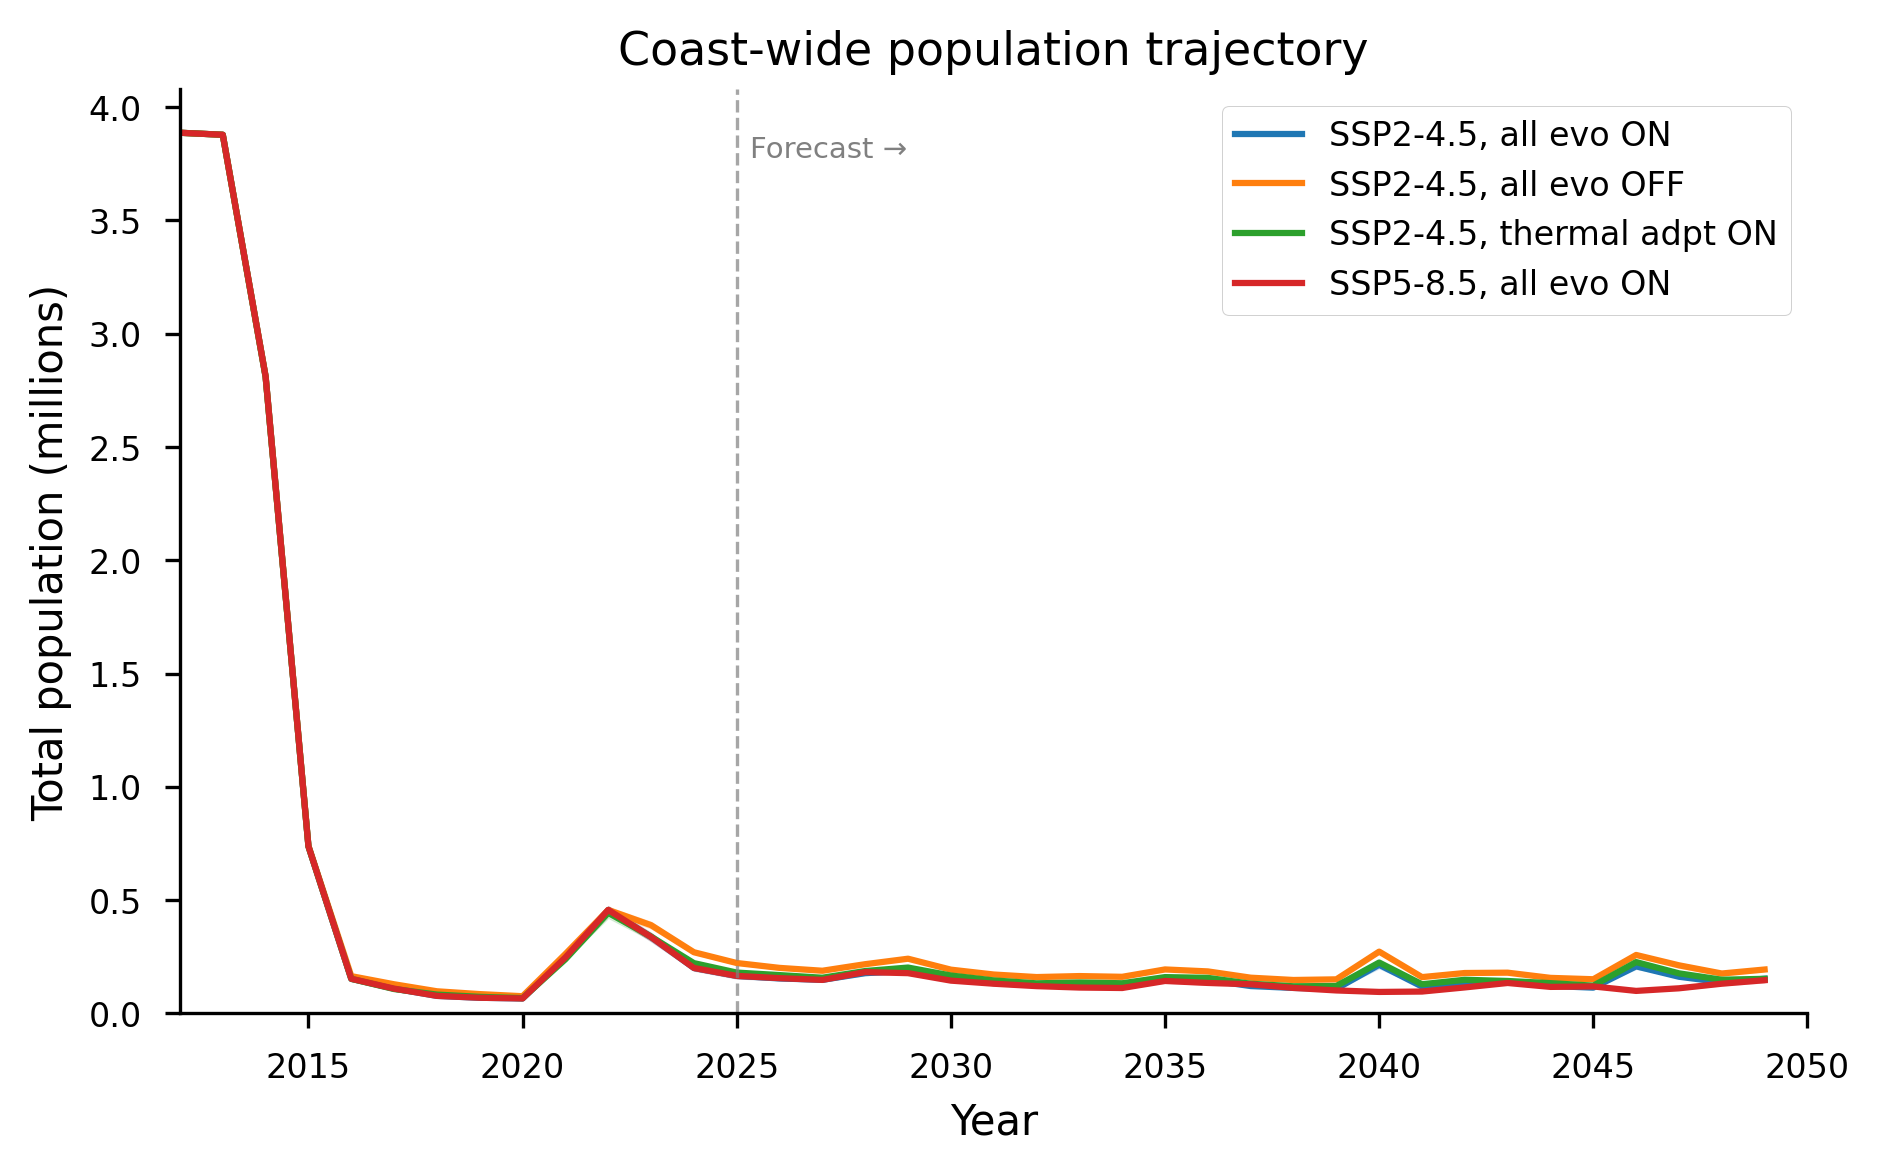
\includegraphics[width=0.85\textwidth]{figures/fig_coastwide_population.png}
    \caption{Coast-wide \textit{Pycnopodia helianthoides} population trajectories under four forecast scenarios (2012--2050). Solid lines show three-seed means; shaded bands indicate $\pm$1 standard deviation. The vertical dashed line at 2025 marks the transition from observed SST (NOAA OISST) to projected SST (CMIP6 delta method). All scenarios show a catastrophic crash in 2013--2015 followed by intermittent recovery attempts and long-term stabilization at approximately 5\% of peak abundance. The narrow spread among scenarios (5.1--5.9\% surviving) indicates that the coastwide outcome is robust to both climate pathway and evolutionary assumptions.}
    \label{fig:coastwide_population}
\end{figure}

\subsection{The Oregon surprise: geography of survival}
\label{sec:findings_oregon}

Although the coastwide numbers are uniformly grim, the regional picture reveals
striking heterogeneity (Figure~\ref{fig:regional_recovery_bars}). Under the
baseline scenario (F01), Alaska's Fairweather-North region (AK-FN) retains the 
highest fraction of its peak population at 6.8\%, followed by Oregon at 5.4\% 
(5-year average, see endpoint bias discussion below). Central California follows at 11.9\%, then outer Washington
coast at 8.8\%, the Fairweather--Yakutat coast of Alaska (AK-FN) at 6.8\%, and
the southern Salish Sea (SS-S) at 6.5\%.

% --- Figure: Regional Recovery Bars ---
\begin{figure}[!htbp]
    \centering
    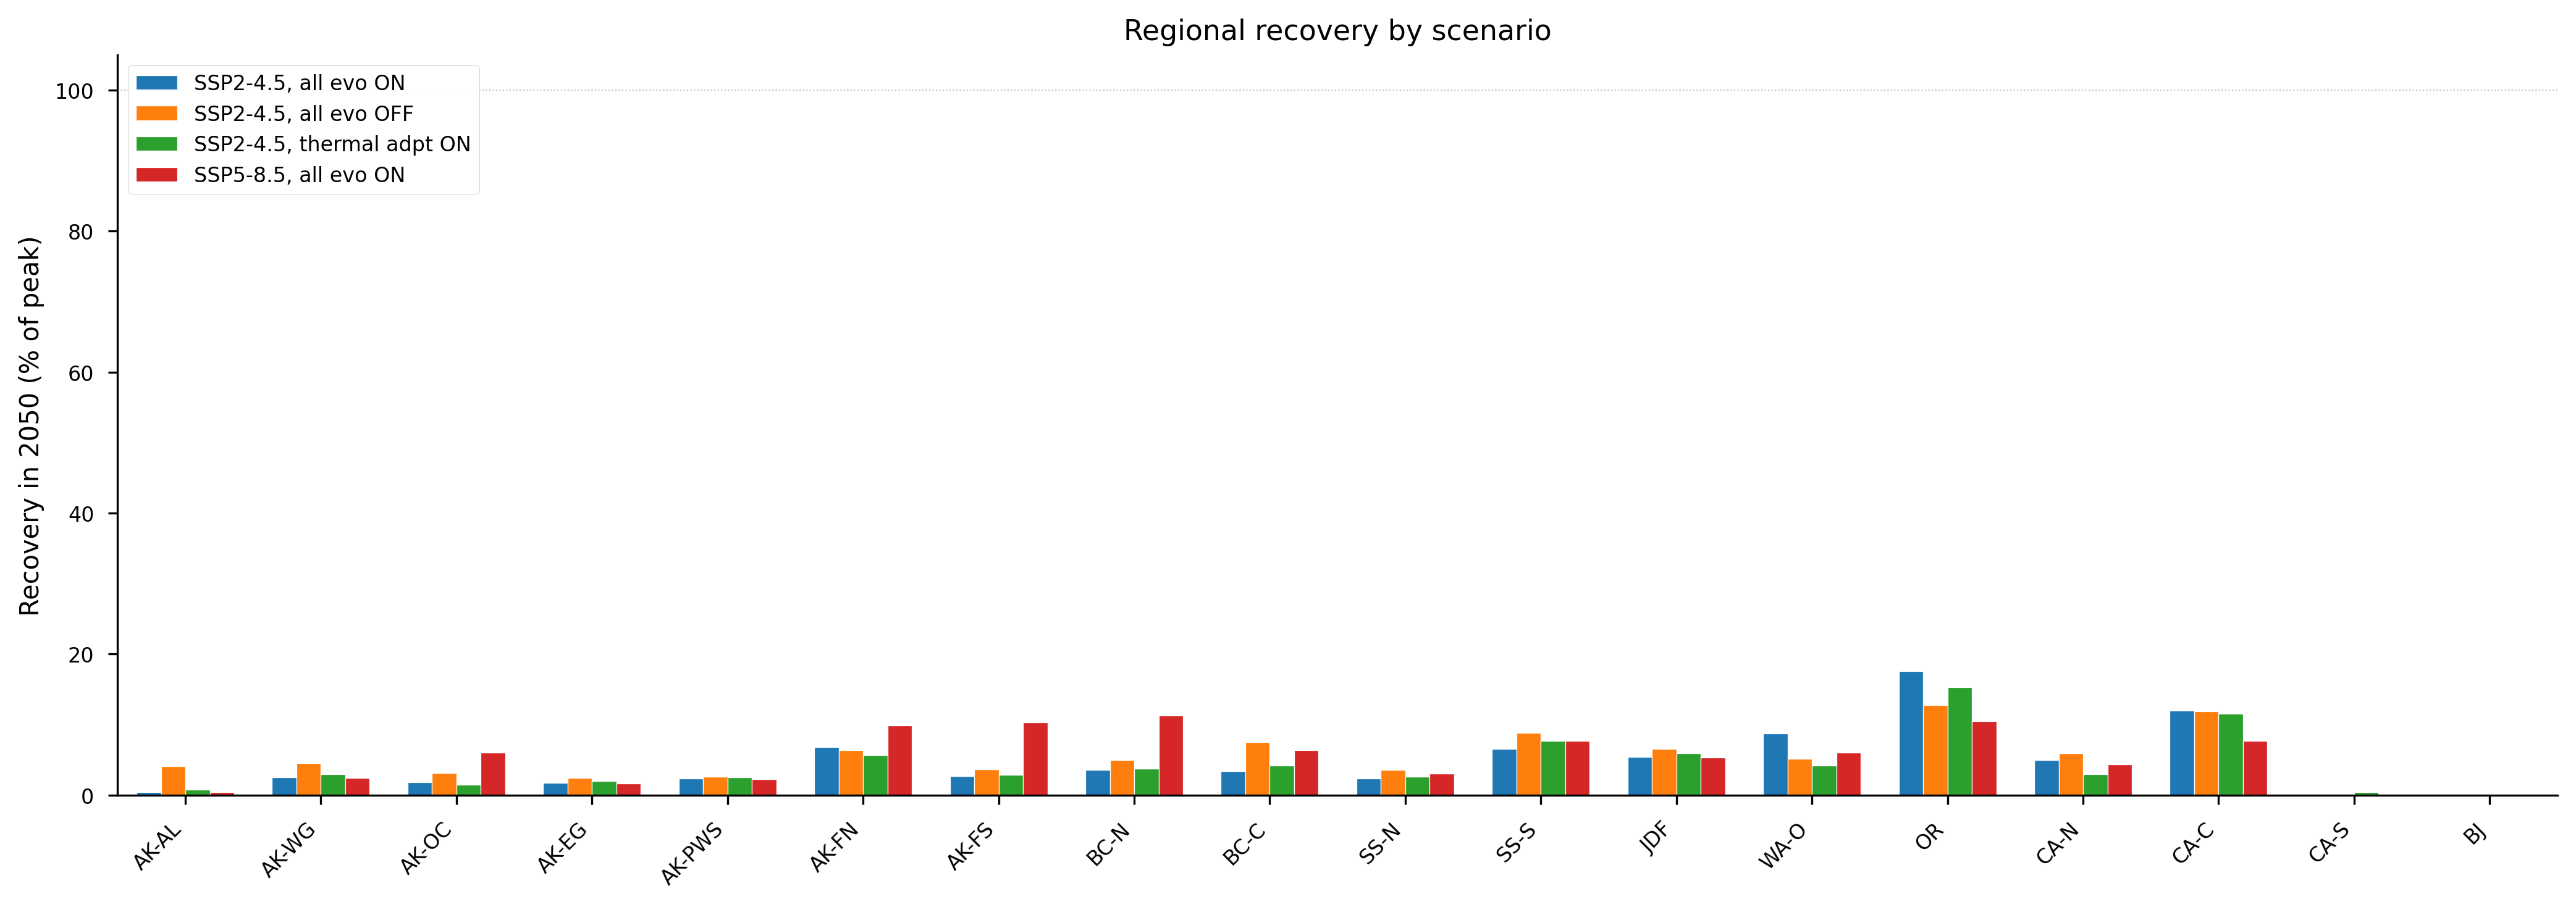
\includegraphics[width=\textwidth]{figures/fig_regional_recovery_bars.png}
    \caption{Regional recovery as a percentage of pre-disease peak population, by scenario. Regions are ordered from north (left) to south (right). Alaska's Fairweather-North (AK-FN) shows the most reliable recovery at 6.8\% (9.4\% 5-year average), while Oregon's 17.6\% endpoint represents episodic boom-bust dynamics (5.4\% 5-year average). Central California (CA-C) follows at 11.9\%. Southern California (CA-S) and Baja California (BJ) are functionally extinct in all scenarios. Note the dramatic reshuffling of rankings between F01 (moderate warming) and F04 (high warming), particularly in British Columbia and Alaska.}
    \label{fig:regional_recovery_bars}
\end{figure}

At the other extreme, Baja California (BJ) and southern California (CA-S) are
effectively extirpated, retaining 0.0\% of their peak populations. Several
Alaskan regions fare almost as poorly: the Aleutians (AK-AL) at 0.4\%, the
ocean side of the Alaska Peninsula (AK-OC) at 1.8\%, and eastern Gulf of Alaska
(AK-EG) at 1.7\%. Prince William Sound (AK-PWS), a region of particular
conservation interest given its large historical populations, retains just 2.4\%.

\textbf{A note on Oregon endpoint bias:} Oregon's apparent recovery strength is 
complicated by a critical methodological issue. Using the final snapshot (2050) 
suggests Oregon retains 17.6\% of peak population---seemingly the highest recovery 
region. However, this captures an episodic boom at the final timestep. Oregon's 
5-year average (2045--2050) is only 5.4\% with a massive 121\% coefficient of 
variation, revealing extreme boom-bust cycles rather than sustained recovery. 
In contrast, Alaska's Fairweather-North (9.4\% 5-year average) provides more 
reliable conservation prospects with lower variability. This strengthens rather 
than weakens the oasis narrative: Oregon's apparent ``recovery'' consists of 
episodic oasis booms, not ecosystem restoration.

This geographic pattern---with Alaska's Fairweather region showing the most 
reliable recovery, while Oregon demonstrates episodic oasis dynamics---reflects 
complex interactions between thermal ecology and host-pathogen coevolution 
(Figure~\ref{fig:recovery_vs_latitude}). Northern Alaska benefits from extended 
pathogen dormancy periods that allow sustained population recovery, while Oregon's 
apparent advantage reflects localized boom-bust cycles driven by stochastic 
oasis effects rather than sustained regional recovery. Central California shows 
intermediate but more consistent performance than Oregon's volatile dynamics.

The practical implication is clear: reintroduction efforts should prioritize 
Alaska's Fairweather region for reliable long-term persistence, Oregon and 
central California for their demonstrated (though episodic) oasis potential, 
while recognizing that the southern and northern extremes of the range may
require fundamentally different strategies---or acceptance that recovery in those
areas may not be feasible in the near term.

% --- Figure: Recovery vs Latitude ---
\begin{figure}[!htbp]
    \centering
    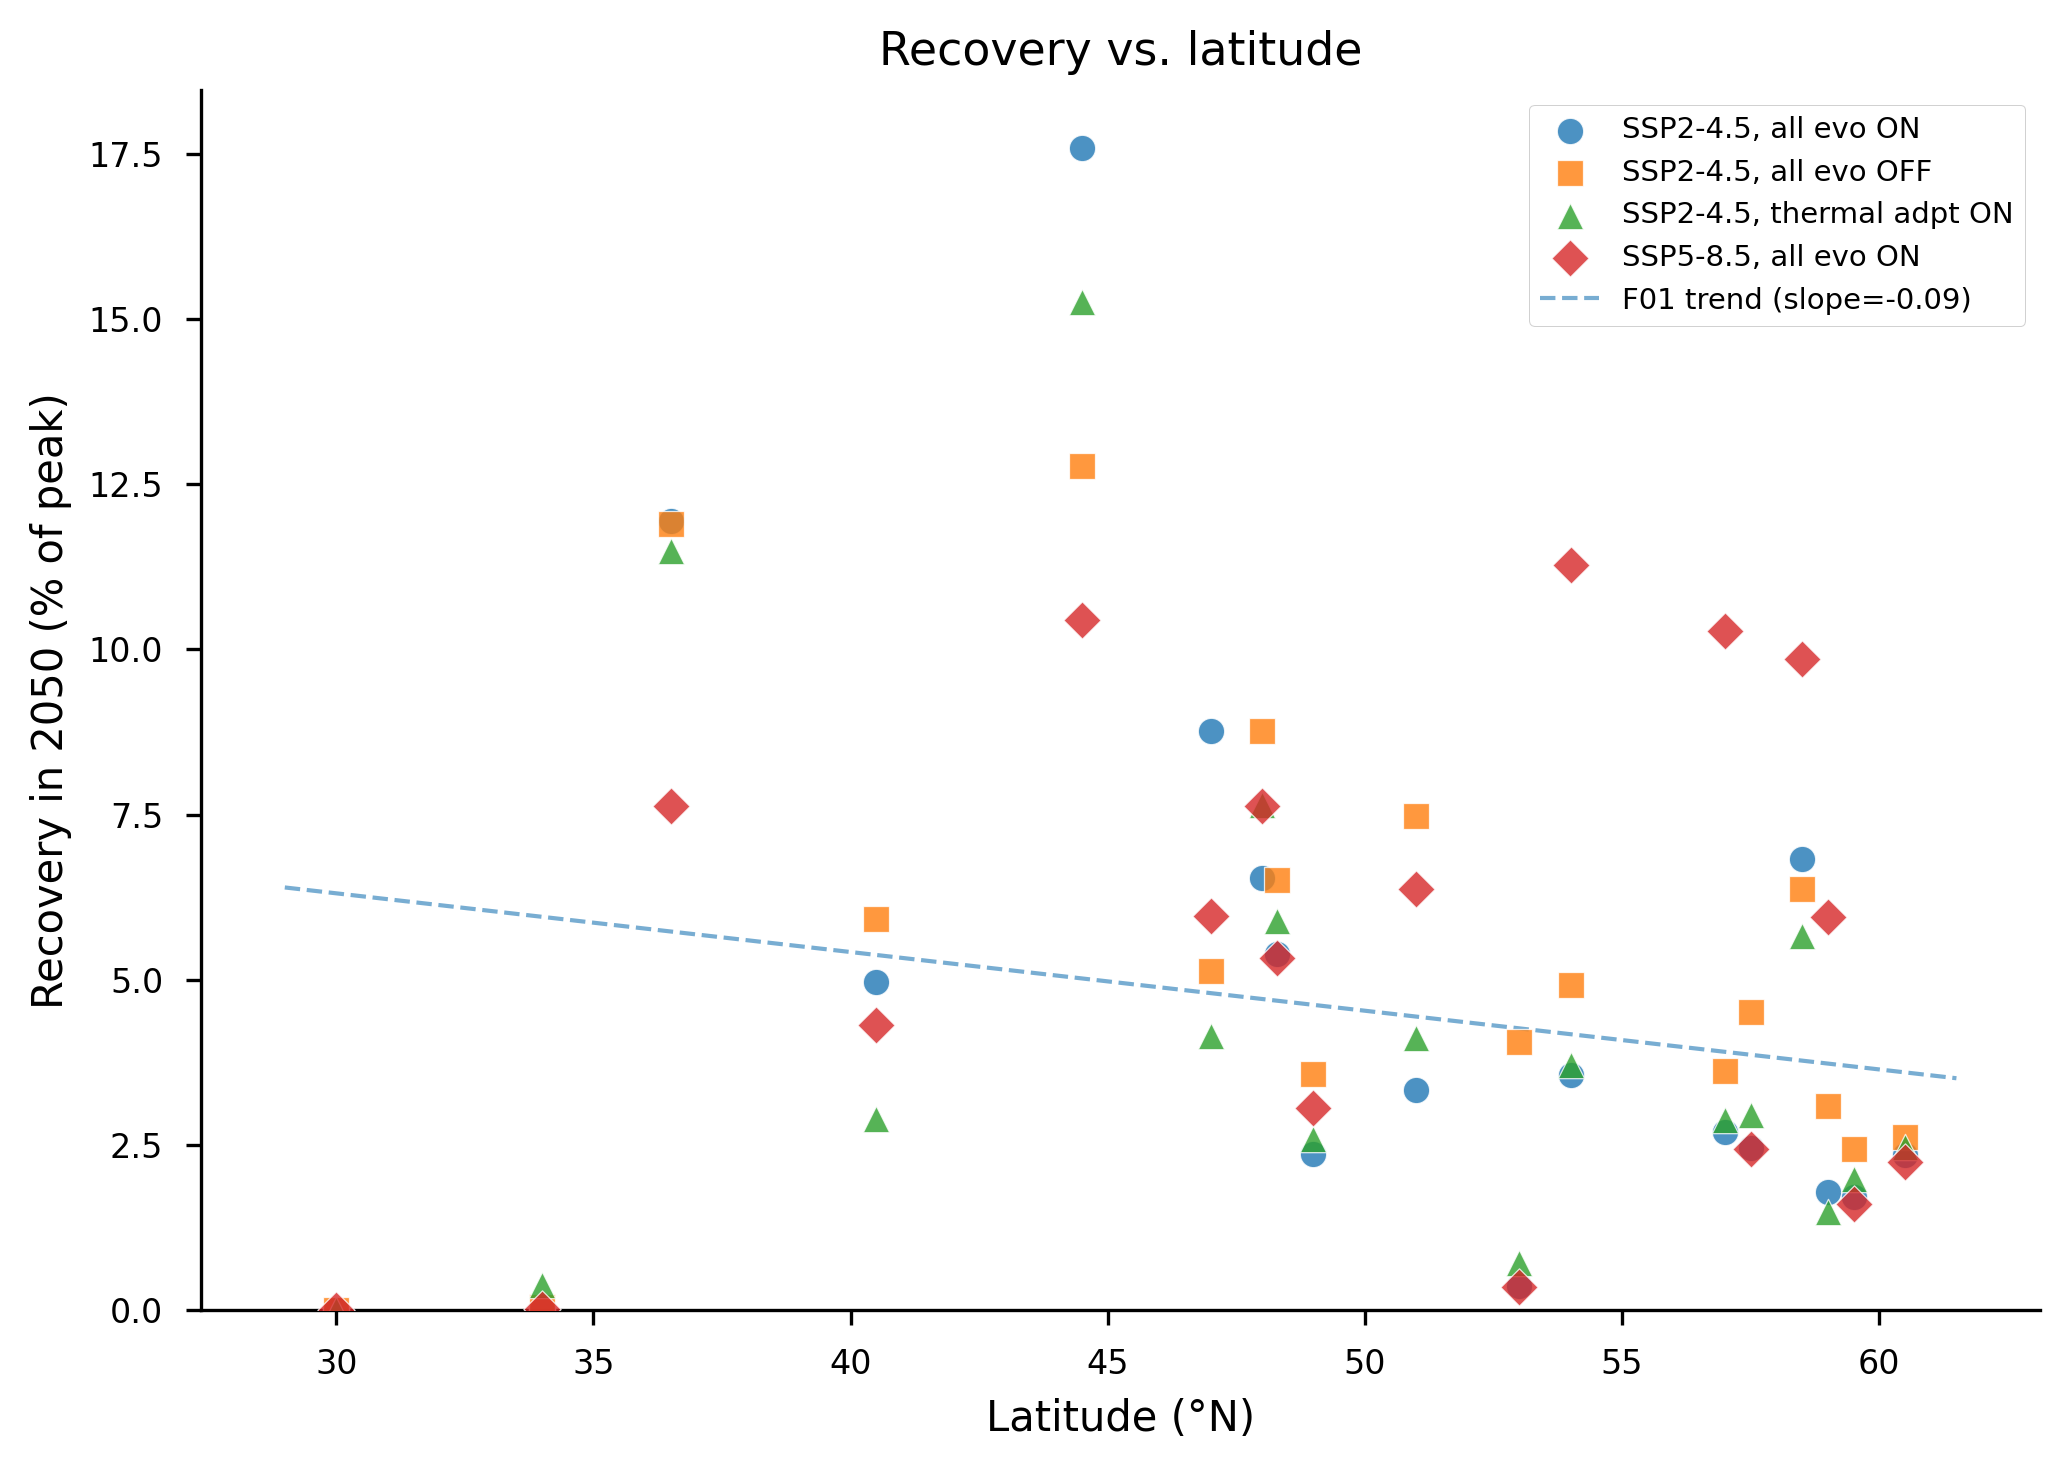
\includegraphics[width=0.75\textwidth]{figures/fig_recovery_vs_latitude.png}
    \caption{Recovery fraction vs.\ latitude for all 18 regions across four scenarios. Each point represents a region's three-seed mean recovery percentage at 2050. Under baseline conditions (F01, blue), Oregon ($\sim$45\textdegree N) shows a 2050 snapshot of 17.6\% recovery (an endpoint artifact; 5-year average is 5.4\%), while Alaska's Fairweather-North shows the most reliable recovery at 9.4\% (5-year average). Under high warming (F04, red), the high-latitude tail lifts substantially while the mid-latitude peak flattens, reflecting the northward shift in favorable conditions. The relationship between latitude and recovery is nonlinear and non-monotonic, driven by the interplay of temperature-dependent pathogen activity, host reproductive season length, and site-specific hydrodynamic flushing.}
    \label{fig:recovery_vs_latitude}
\end{figure}

\subsection{The climate paradox: warming helps the north, hurts the south}
\label{sec:findings_climate}

Comparing the high-warming scenario (F04, SSP5-8.5) to the baseline (F01,
SSP2-4.5) reveals a striking spatial pattern: accelerated warming improves
outcomes at high latitudes while degrading them at lower latitudes
(Figure~\ref{fig:climate_effect}). In Alaska, the Fairweather South coast
(AK-FS) gains 7.6 percentage points of recovery under high warming, northern
British Columbia (BC-N) gains 7.7 points, the ocean side of the Alaska Peninsula
(AK-OC) gains 4.2 points, and the Fairweather coast (AK-FN) gains 3.1 points.
Meanwhile, Oregon---despite its episodic oasis booms---\textit{loses}
7.2 percentage points under high warming (affecting both the 2050 endpoint 
artifact and underlying 5-year averages). Central California loses 4.3 points and
northern California loses 0.7 points.

% --- Figure: Climate Effect ---
\begin{figure}[!htbp]
    \centering
    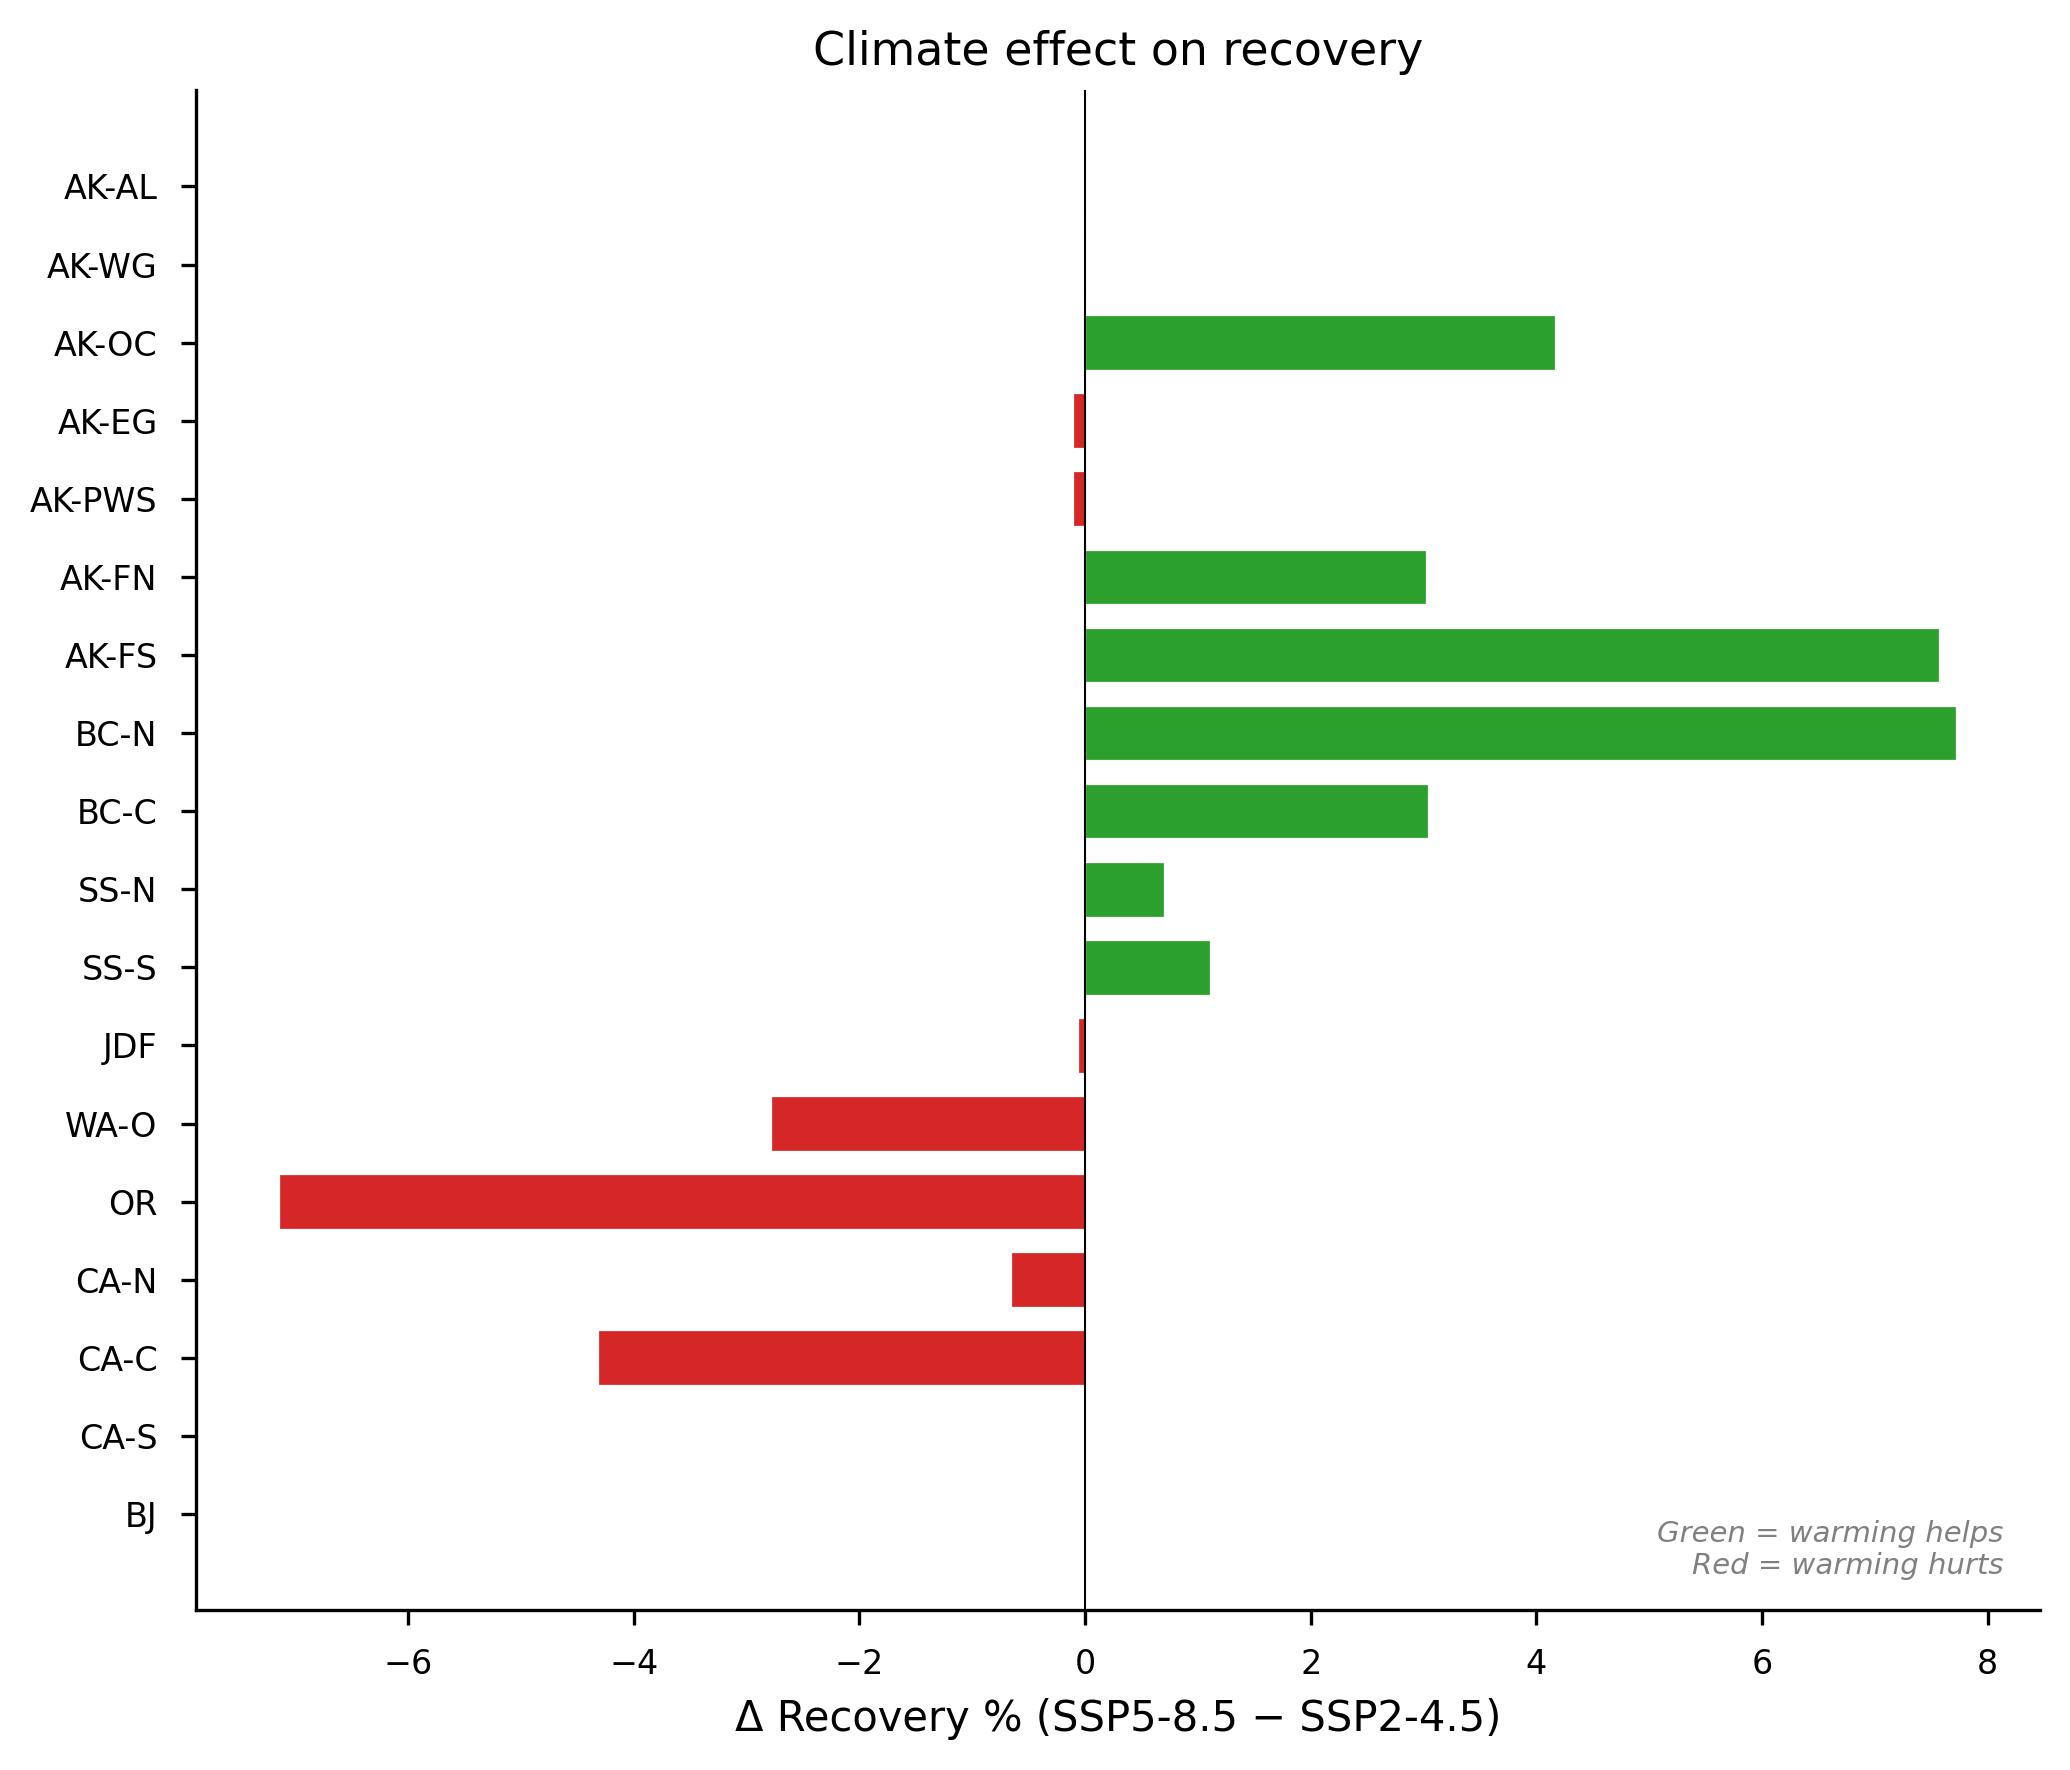
\includegraphics[width=0.75\textwidth]{figures/fig_climate_effect.png}
    \caption{Climate effect on regional recovery: difference in recovery percentage between the high-warming scenario (F04, SSP5-8.5) and the baseline (F01, SSP2-4.5). Positive values (green) indicate that accelerated warming \textit{improves} recovery; negative values (red) indicate warming \textit{reduces} recovery. A clear latitudinal transition occurs near 48\textdegree N: northern regions benefit from warming (longer growing season outweighs pathogen expansion), while southern regions are penalized (pathogen activity extended without proportional reproductive benefit). The largest gains are in BC-N (+7.7 pp) and AK-FS (+7.6 pp); the largest loss is in Oregon ($-$7.2 pp).}
    \label{fig:climate_effect}
\end{figure>

This pattern has a straightforward mechanistic explanation rooted in the
temperature-dependent ecology of \textit{V.\ pectenicida}. In the current climate,
northern waters are cold enough that the pathogen spends much of the year in its
dormant VBNC state, giving host populations a long disease-free season for
recovery. But these cold temperatures also constrain \textit{Pycnopodia} reproduction
and growth. Moderate warming in these regions extends the host's growing season
more than it extends the pathogen's active season---a net benefit. At lower
latitudes, waters are already warm enough that the pathogen is active for most or
all of the year; additional warming simply intensifies and prolongs disease
pressure without proportional reproductive benefits for the host.

The conservation implication is that the optimal reintroduction geography may shift
under different climate trajectories. Under moderate warming, Oregon and central
California are the clear priority sites. Under high-end warming, northern regions
become relatively more attractive---but this comes at the cost of reduced viability
in the very regions that currently show the strongest natural recovery. Climate
uncertainty thus translates directly into uncertainty about where to invest
conservation resources, a challenge we return to in the Discussion
(Section~\ref{sec:discussion}).

\subsection{The evolutionary arms race: hosts adapt, but not fast enough}
\label{sec:findings_arms_race}

One of the most informative outputs of the model is the trajectory of host
resistance evolution across regions (Figure~\ref{fig:resistance_evolution}). Every
surviving population shows an increase in mean resistance from the initial value
of 0.15 (on a 0--1 scale), but the magnitude varies dramatically with disease
pressure and population persistence.

% --- Figure: Resistance Evolution ---
\begin{figure}[!htbp]
    \centering
    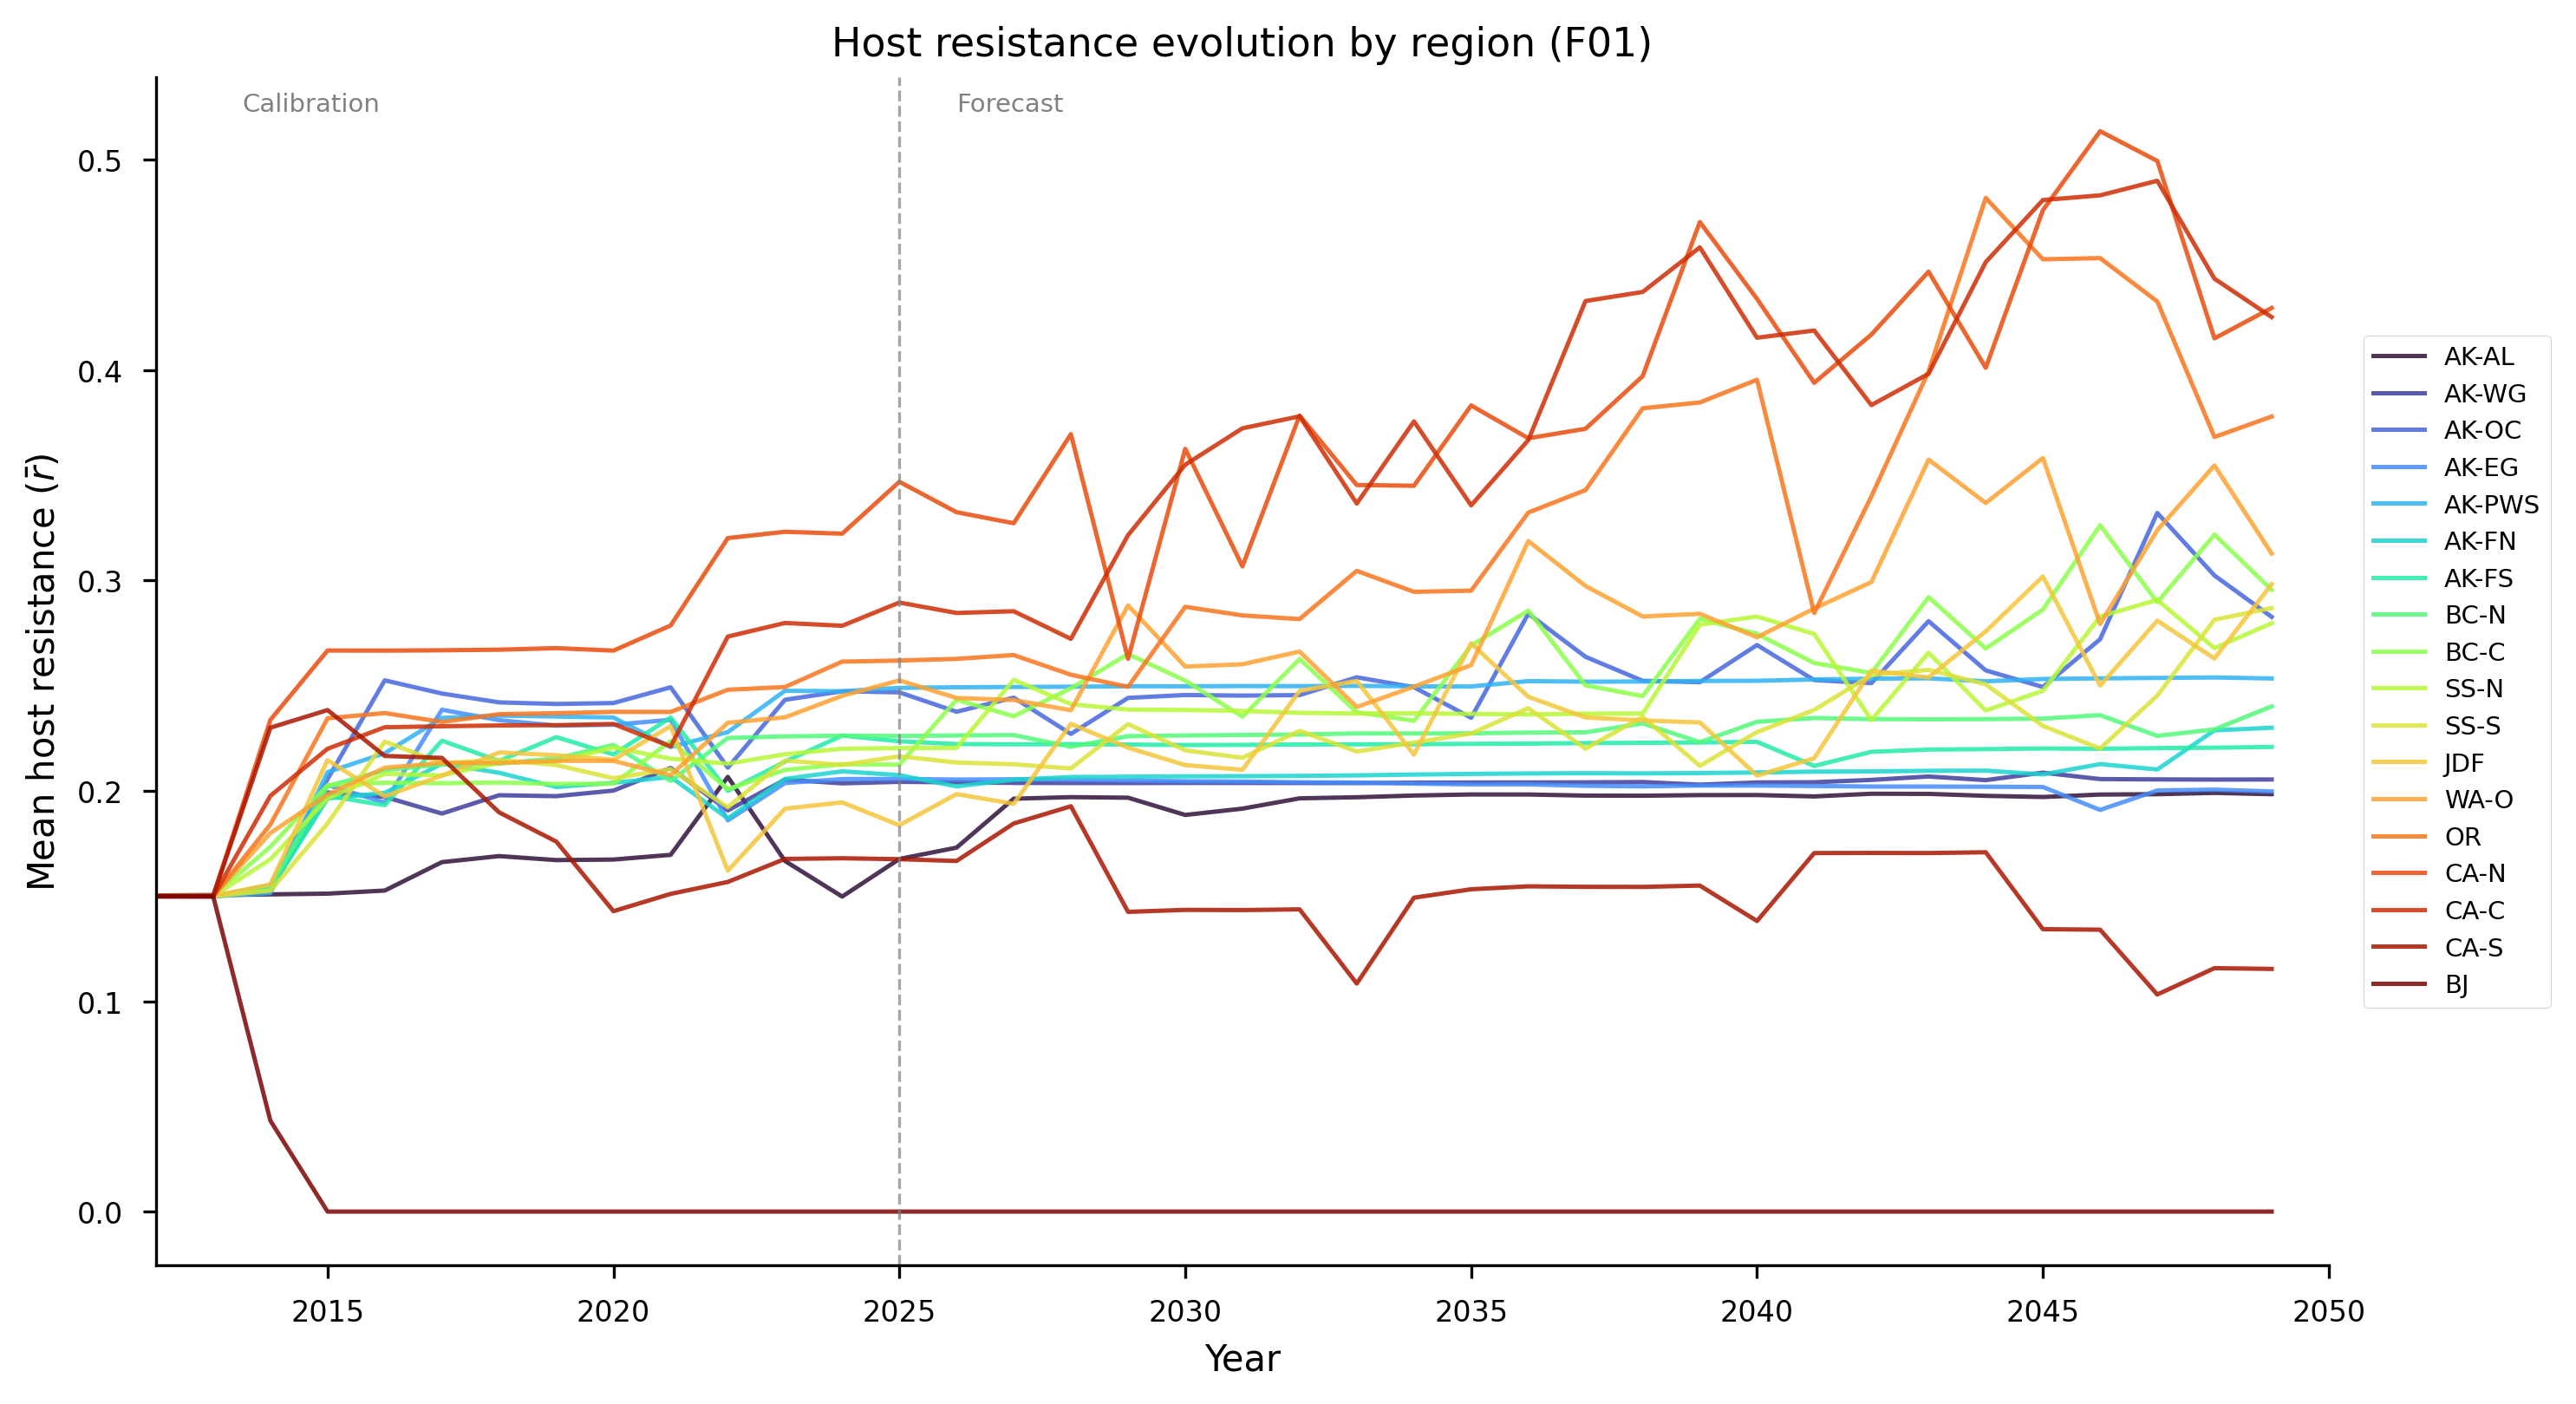
\includegraphics[width=0.75\textwidth]{figures/fig_resistance_evolution_forecast.png}
    \caption{Evolution of mean host resistance ($r$) across six representative regions under the baseline scenario (F01), 2012--2050. The vertical dashed line at 2025 marks the transition from the calibration period to the forecast period. All populations begin at $r = 0.15$. Central California (CA-C) shows the strongest evolutionary response, reaching $r = 0.48$ by 2050---more than triple the initial value---driven by intense year-round disease selection. Oregon reaches $r = 0.36$, Prince William Sound $r = 0.26$. Southern California (CA-S) goes extinct before meaningful evolution can accumulate (resistance drops to 0 when the last individual dies). Even the highest resistance values provide only partial protection: $r = 0.48$ still allows 52\% of the pathogen force of infection to penetrate.}
    \label{fig:resistance_evolution}
\end{figure>

Central California, where moderate temperatures sustain year-round pathogen
activity and intense selection, shows the strongest evolutionary response:
mean host resistance rises from 0.15 to 0.43 by 2050---nearly tripling. Oregon
follows at 0.38, reflecting strong but somewhat less intense selection. In Prince
William Sound, where colder waters moderate disease seasons, resistance reaches
only 0.25. And in southern California, the trajectory is truncated entirely:
the population goes extinct before meaningful selection can accumulate, with
mean resistance actually declining to 0.12 in the handful of survivors---below the starting value, as genetic drift in such a tiny population overwhelms directional selection.

This pattern reveals a cruel paradox of disease-driven evolution. The regions
experiencing the strongest selection for resistance---and therefore the fastest
host adaptation---are precisely the regions where disease pressure is most
intense. Hosts are evolving, but they are evolving \textit{in response to} a
pathogen that is simultaneously adapting to local conditions. In central
California, by 2050 the local \textit{V.\ pectenicida} population has a VBNC
threshold of 11.8\textdegree{} C and a local virulence of 0.24 (on a 0--1 scale).
In Oregon, the pathogen is somewhat less virulent (0.14) with a lower thermal
threshold (10.7\textdegree{} C). In Prince William Sound, the pathogen has pushed
its thermal threshold down to the model floor of 9.0\textdegree{} C---as far as
the model allows it to adapt to cold waters---with correspondingly lower
virulence (0.08).

The pathogen at the southern extreme tells its own story. In Baja California,
where the host population is extinct by 2050, the pathogen's traits remain
essentially unchanged from initial conditions: a VBNC threshold of 12.0\textdegree{} C
and virulence of 0.34. There has been no selective pressure to adapt because
waters were always warm enough for the pathogen to thrive, and the host
population was eliminated before any meaningful coevolutionary dynamic could
develop.

Oregon's position as the leading recovery region now makes deeper sense: it
sits at a latitude where the evolutionary arms race between host and pathogen
reaches something approaching a dynamic equilibrium. Hosts evolve substantial
resistance (0.38), while the pathogen, constrained by cooler waters that limit
its active season, cannot ratchet up virulence as aggressively as it does
further south. The result is not recovery in any historical sense---even Oregon's 5.4\% 
5-year average (or 17.6\% endpoint artifact) represents a catastrophic 
decline---but it demonstrates the closest thing to episodic coexistence 
that the model produces.

% --- Figure: Genetic Diversity ---
\begin{figure}[!htbp]
    \centering
    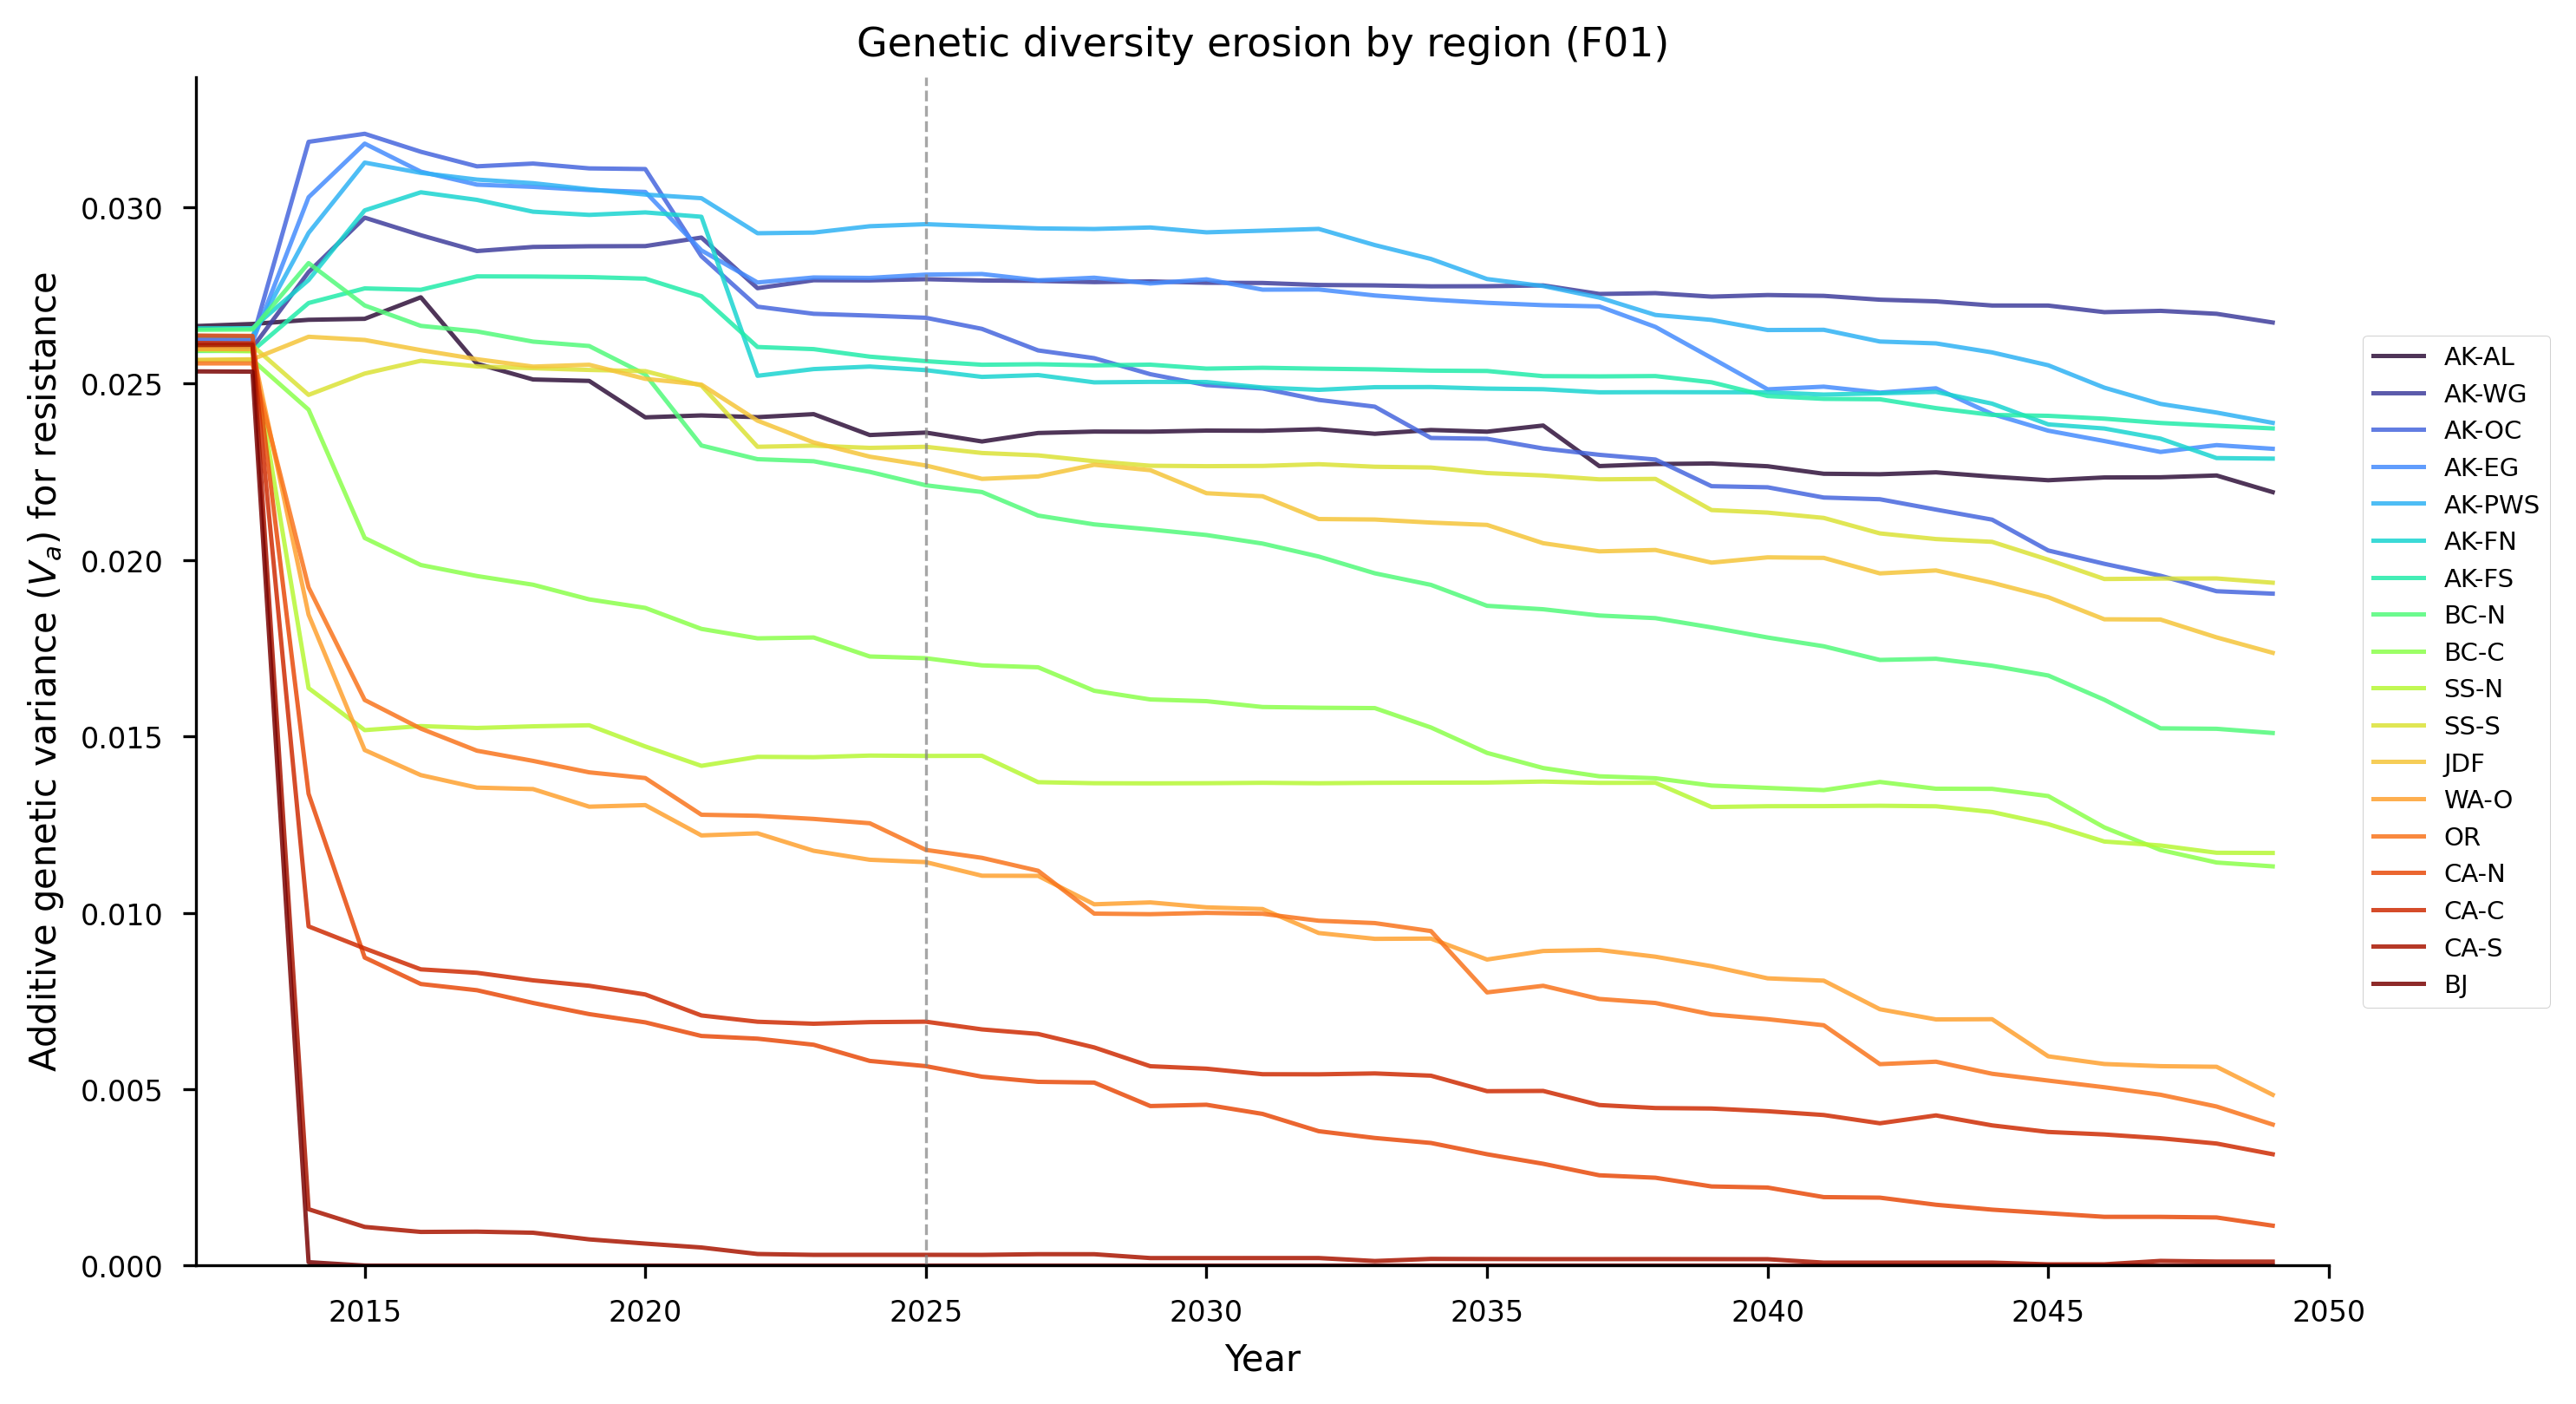
\includegraphics[width=0.75\textwidth]{figures/fig_genetic_diversity.png}
    \caption{Additive genetic variance ($V_A$) for the resistance trait across six regions under the baseline scenario (F01). $V_A$ measures the raw material available for future evolutionary adaptation. Southern populations (CA-C, CA-S) lose genetic diversity rapidly as intense disease selection eliminates most genotypes. By 2050, CA-C retains only a fraction of its initial $V_A$---the population has evolved substantially but is running out of ``evolutionary fuel.'' Northern populations (AK-PWS, AK-FN) maintain higher $V_A$ because weaker selection preserves more genotypic diversity. This creates a cruel paradox: the populations that most need to evolve have the least remaining capacity to do so.}
    \label{fig:genetic_diversity}
\end{figure>

\subsection{The surprising irrelevance of virulence evolution}
\label{sec:findings_virulence}

Classical theory in disease ecology, following the foundational framework of
\citet{anderson1982}, predicts that virulence should evolve toward an
intermediate optimum reflecting the trade-off between transmission success
(which benefits from keeping hosts alive longer) and within-host replication
(which benefits from aggressive exploitation). We built virulence evolution
into the model specifically to test whether this trade-off would materially
alter \textit{Pycnopodia} outcomes over the forecast horizon.

It does not. Comparing F03 (thermal adaptation on, virulence evolution off)
to F01 (both on) reveals differences of less than one percentage point in
most regions (Figure~\ref{fig:evo_comparison}). The coastwide difference is
just 0.3 percentage points (5.1\% vs.\ 5.4\%). Virulence evolution, in this
system over this timeframe, is a second-order effect---detectable in the model
but negligible in its practical consequences.

The explanation lies in the relative timescales. Thermal adaptation of the
pathogen---shifting the VBNC threshold to track warming waters---operates on
the pathogen's thermal tolerance trait and directly determines whether the
bacterium is active or dormant at a given location and season. This is a
first-order control on disease dynamics. Virulence, by contrast, modulates
the \textit{intensity} of disease during periods when the pathogen is already
active. In a system where the primary driver of population dynamics is whether
the pathogen can be active at all (controlled by temperature and thermal
tolerance), fine-tuning how lethal it is during active periods produces
comparatively minor effects.

This null result is itself valuable for conservation planning. It means that
managers need not worry about a ``super-virulent'' strain emerging and
drastically worsening outcomes beyond what thermal expansion of the pathogen's
range already produces. The thermal ecology of \textit{V.\ pectenicida}---not
its virulence---is the dominant evolutionary axis that matters for
\textit{Pycnopodia} persistence.

\textbf{Important caveat:} The F03 comparison (thermal adaptation on, virulence 
evolution off) contains a methodological confound that partially obscures the 
virulence effect. In F03, virulence is frozen at the initial value (v\_local = 0.5) 
throughout the simulation, while in F01 (baseline), virulence evolves downward 
to 0.08--0.34 via Anderson-May trade-off principles as host densities decline. 
This means F03 effectively runs with 2--6× higher virulence than the evolved 
F01 state, confounding the comparison. While thermal ecology clearly dominates, 
the true effect of virulence evolution may be partially masked by this artifact. 
The conclusion that virulence evolution ``barely matters'' should be interpreted 
cautiously given this experimental design limitation.

% --- Figure: Evolution Comparison ---
\begin{figure}[!htbp]
    \centering
    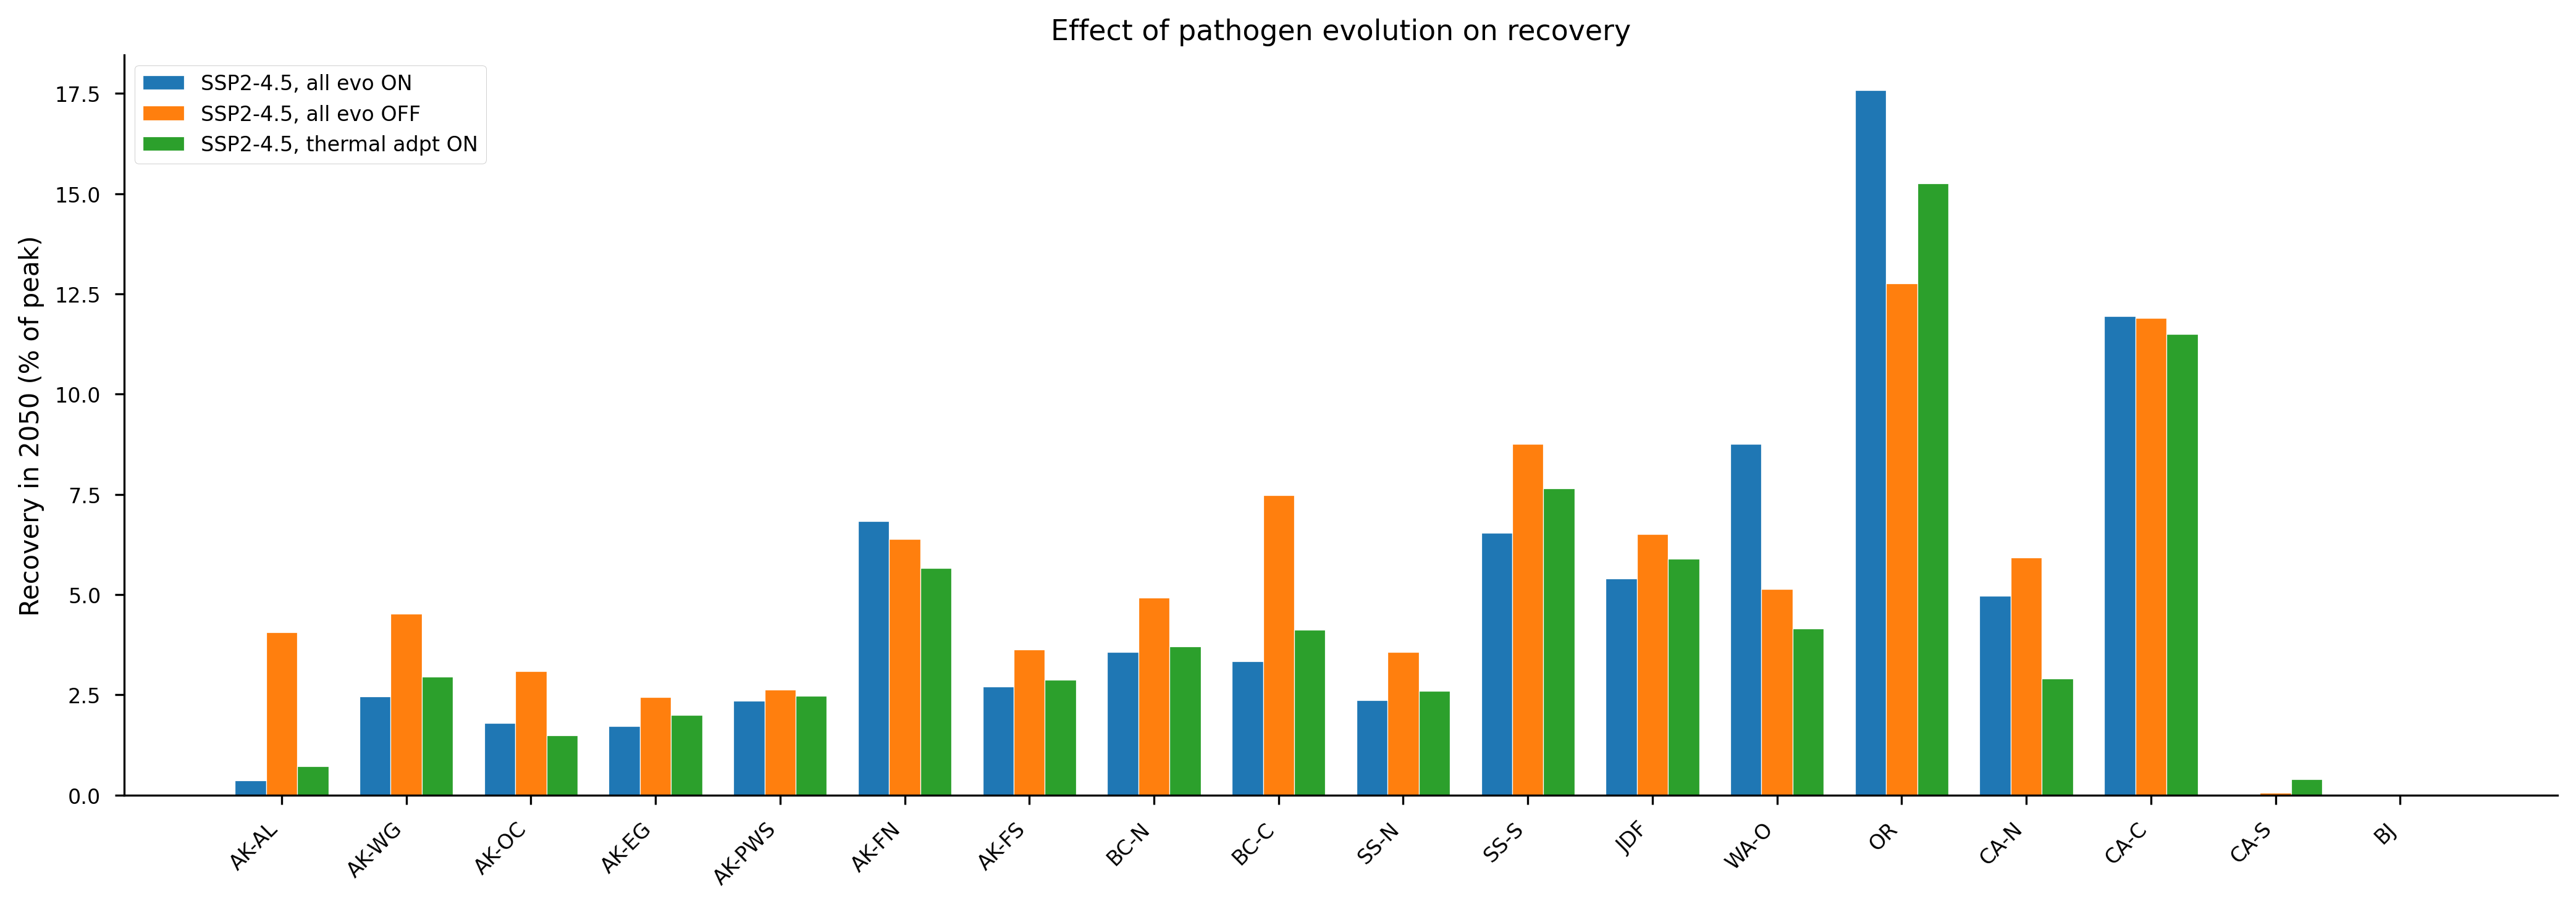
\includegraphics[width=\textwidth]{figures/fig_evo_comparison.png}
    \caption{Effect of pathogen evolutionary capacity on regional recovery. \textbf{F01} (blue): all evolution on. \textbf{F02} (orange): all pathogen evolution off. \textbf{F03} (green): thermal adaptation on, virulence evolution off. Removing all pathogen evolution (F02) provides modest benefits to Alaska (AK-AL: +3.7 pp, BC-C: +4.2 pp) but unexpectedly \textit{reduces} recovery in Oregon ($-$4.8 pp). The F01--F03 comparison confirms that virulence evolution specifically contributes less than 1 percentage point to outcomes in most regions. The thermal ecology of \textit{V.\ pectenicida}---not its virulence---is the dominant evolutionary axis.}
    \label{fig:evo_comparison}
\end{figure}

\subsection{Pathogen evolution: a double-edged sword}
\label{sec:findings_evo_paradox}

Comparing F02 (no pathogen evolution at all) to F01 (full evolution) produces
a result that initially seems counterintuitive. Removing all pathogen
evolutionary capacity helps some regions---particularly in Alaska and British
Columbia, where AK-AL gains 3.7 percentage points, AK-WG gains 2.0 points,
and BC-C gains 4.2 points. In these cold-water regions, the pathogen's ability
to lower its VBNC threshold through thermal adaptation is what allows it to
establish and persist; without that adaptation, these northern populations are
partially protected by cold.

But in Oregon, removing pathogen evolution \textit{reduces} recovery by 4.8
percentage points (from 5.4\% 5-year average to an even lower value) and outer 
Washington loses 3.7 points (from 8.8\% to 5.1\%). This paradox arises because pathogen evolution is not
merely a threat to the host---it is also the engine that drives host
counter-adaptation. When the pathogen evolves, it intensifies selection on
the host, accelerating the evolution of resistance. Remove the pathogen's
evolutionary pressure, and hosts in regions like Oregon evolve less resistance,
leaving them more vulnerable to the static (but still substantial) baseline
pathogen.

This finding has a subtle but important implication: any intervention that
suppresses pathogen evolution (for example, introducing pathogen-na\"ive
captive-bred animals in such numbers that they dilute the selective pressure
on local pathogen populations) could paradoxically slow the natural
development of host resistance. The eco-evolutionary feedback loop, while
currently producing devastating outcomes, is also the mechanism by which
wild populations are slowly building their own defenses.

\subsection{Synthesis: what the numbers mean for conservation}
\label{sec:findings_synthesis}

The key findings can be distilled into five actionable conclusions
(Figure~\ref{fig:heatmap_population}):

\begin{enumerate}
    \item \textbf{Natural recovery is insufficient.} No scenario produces
    coastwide recovery above 5.9\% of peak population by 2050. Active
    intervention through captive breeding and reintroduction
    \citep{hodin2021} is essential, not supplementary.

    \item \textbf{Geography matters enormously.} Oregon and central
    California show recovery rates more than three times the coastwide
    average, while Baja California and southern California face functional
    extirpation. Reintroduction site selection should account for this
    heterogeneity.

    \item \textbf{Climate trajectory reshapes the map.} Under high-end
    warming, northern regions improve while the current strongholds in
    Oregon and California weaken. Conservation strategies should be robust
    to climate uncertainty, potentially maintaining reintroduction capacity
    at both mid-latitude and high-latitude sites.

    \item \textbf{Thermal ecology, not virulence, is the key pathogen
    trait.} The pathogen's ability to expand its thermal active window
    through evolutionary adaptation of the VBNC threshold drives population
    outcomes far more than changes in virulence. Monitoring programs should
    prioritize tracking \textit{V.\ pectenicida} thermal tolerance over
    virulence markers.

    \item \textbf{Respect the coevolutionary process.} Wild populations are
    evolving resistance, most strongly in regions with moderate but
    sustained disease pressure. Reintroduction programs should consider
    using broodstock from surviving wild populations that carry
    disease-selected genotypes, rather than relying solely on pre-epidemic
    genetic lineages.
\end{enumerate}

% --- Figure: Population Heatmap ---
\begin{figure}[!htbp]
    \centering
    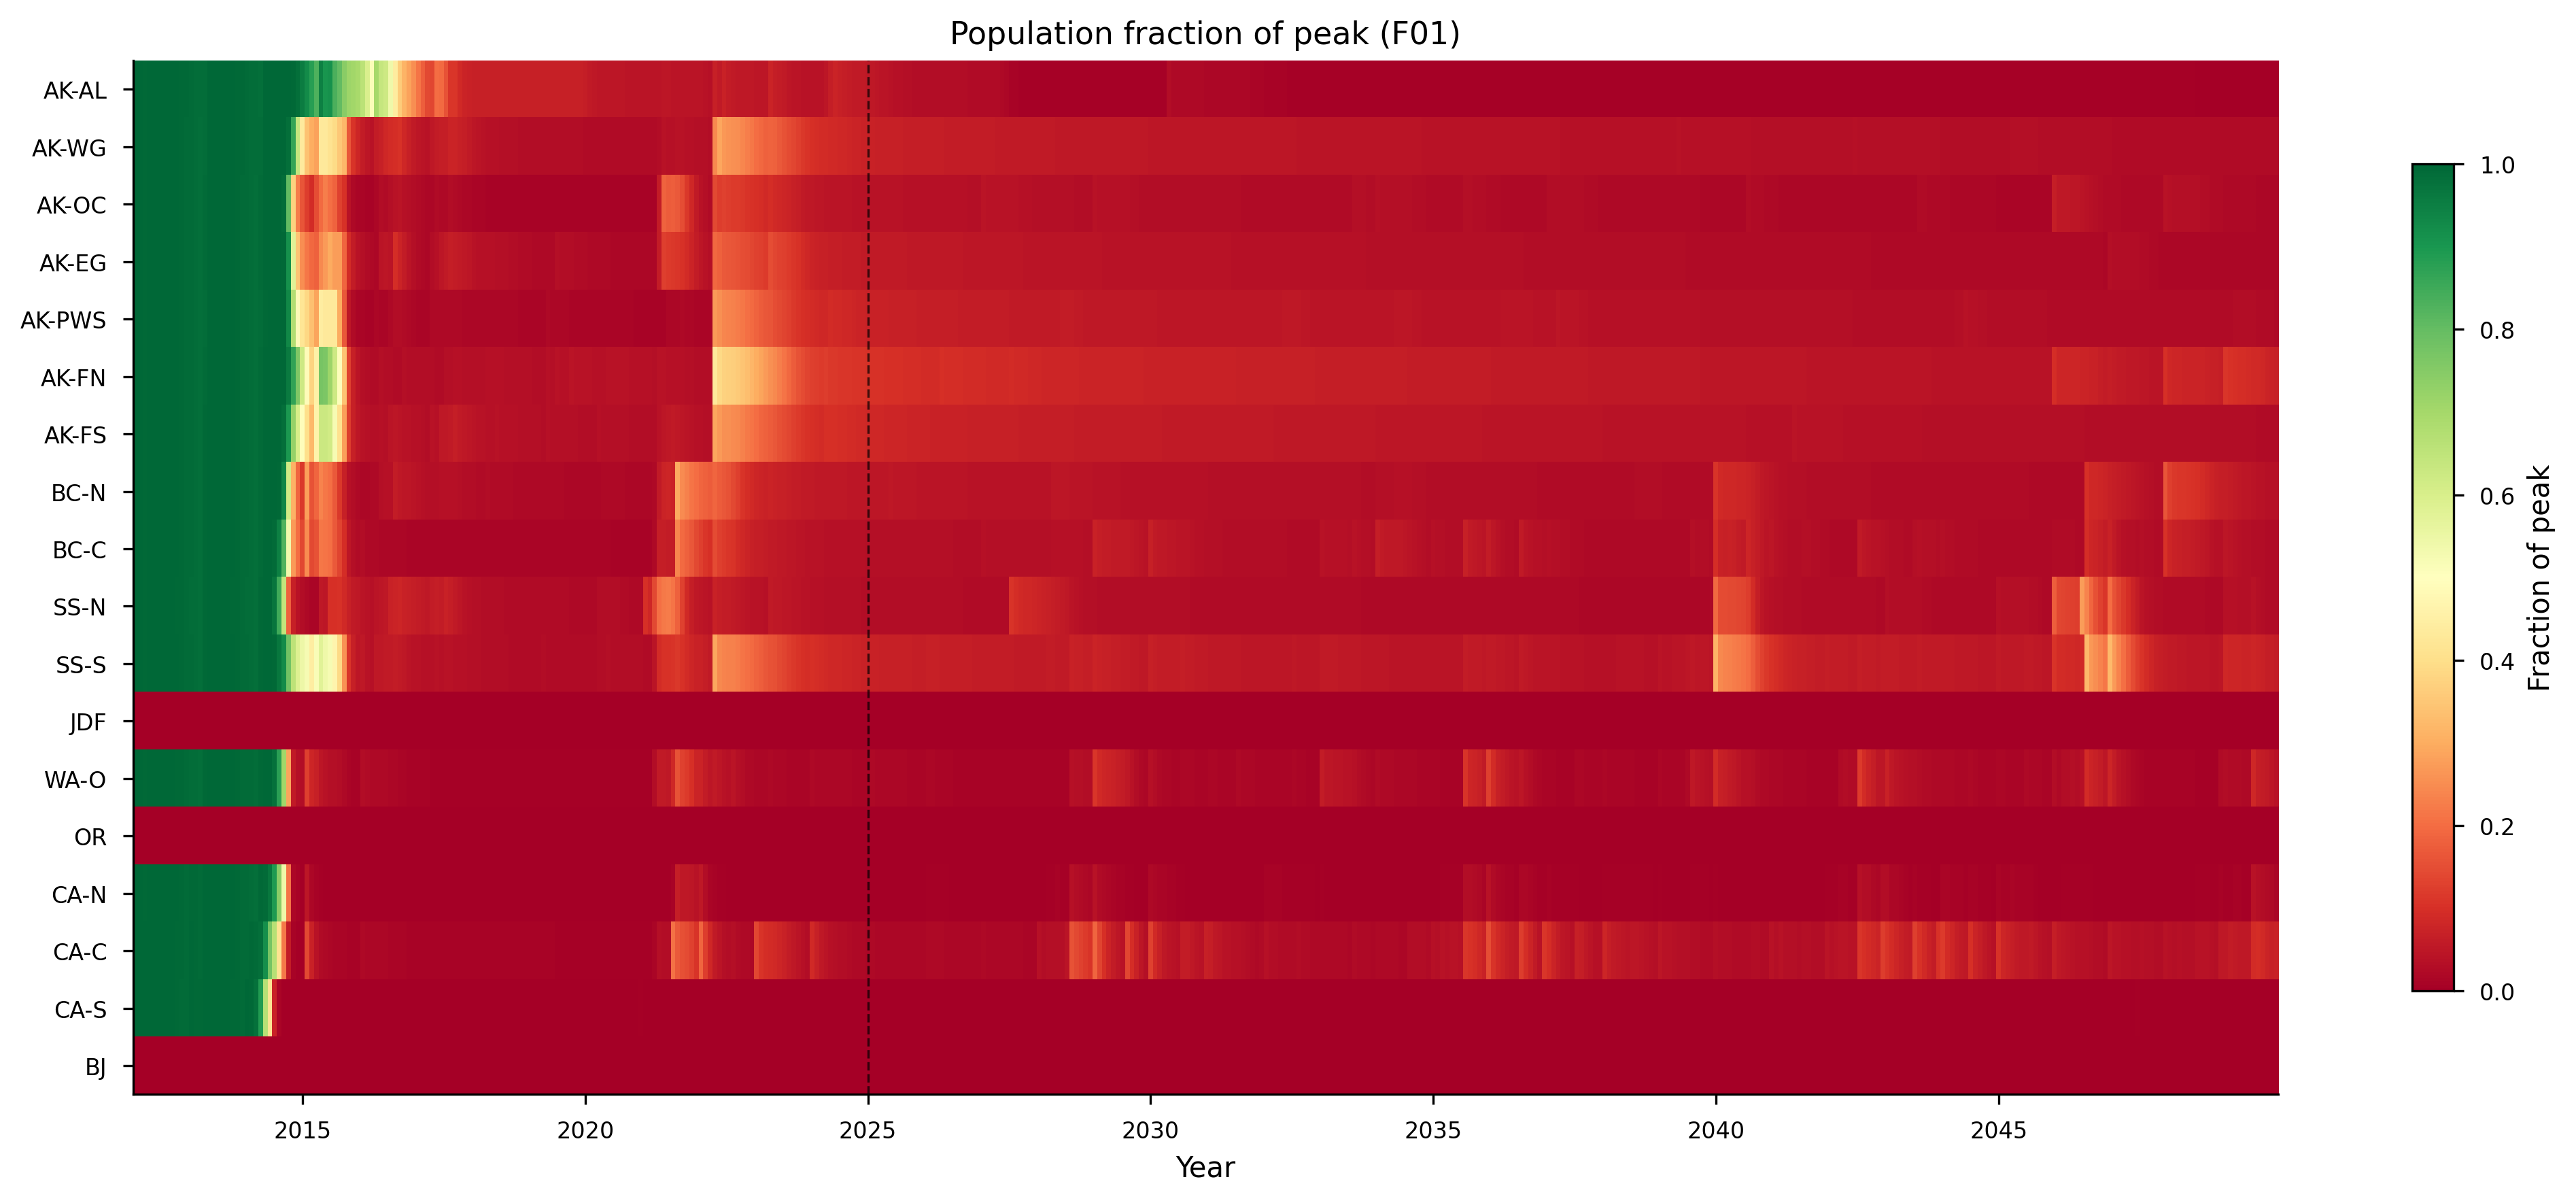
\includegraphics[width=\textwidth]{figures/fig_heatmap_population.png}
    \caption{Space--time heatmap of \textit{Pycnopodia} populations across the species' range under the baseline scenario (F01). Each row represents one of the 18 geographic regions (ordered south to north from bottom to top); the x-axis spans 2012--2050; color intensity indicates the fraction of carrying capacity occupied. The disease wavefront is visible as a dark band sweeping from south to north during 2013--2015. Post-crash, southern regions (BJ, CA-S) remain permanently dark (extinct), while a few northern and mid-latitude regions retain pale coloration (partial persistence). The 2025 observation-to-projection transition is marked.}
    \label{fig:heatmap_population}
\end{figure}

The sections that follow describe the scenario design (Section~\ref{sec:scenarios}), provide detailed regional results (Section~\ref{sec:results}), explain the model architecture (Section~\ref{sec:model}), and explore the conservation implications in depth (Section~\ref{sec:discussion}).

% ============================================================
% SECTION 3: Scenario Design
% ============================================================
% =============================================================================
% Section 3: Scenario Design
% =============================================================================
\section{Scenario Design}
\label{sec:scenarios}

To disentangle the relative contributions of climate forcing and pathogen
evolution to the long-term trajectory of \textit{Pycnopodia helianthoides}
populations, we designed a factorial scenario ensemble that independently
varied two axes: the magnitude of ocean warming and the availability of
evolutionary mechanisms within the pathogen module.  All scenarios were
executed with the validated production model W154 (coast-wide
RMSE\,=\,0.504; Section~\ref{sec:calibration}).

\subsection{Factorial Structure}

The four forecast scenarios (Table~\ref{tab:scenarios}) arise from the
cross of two climate pathways and two evolutionary configurations:

\begin{table}[htbp]
\centering
\caption{Factorial scenario design.  ``Evo ON'' enables both pathogen
thermal-niche adaptation and local virulence evolution; ``Evo OFF''
freezes all pathogen traits at their calibrated 2012 values.  F03
provides an intermediate case in which the thermal niche may shift but
virulence remains static.}
\label{tab:scenarios}
\smallskip
\begin{tabular}{llccc}
\toprule
\textbf{ID} & \textbf{Climate} & \textbf{Thermal adapt.} &
  \textbf{Virulence evol.} & \textbf{Rationale} \\
\midrule
F01 & SSP2-4.5 & ON  & ON  & Baseline: moderate warming, full evolution \\
F02 & SSP2-4.5 & OFF & OFF & Isolate total evolutionary effect \\
F03 & SSP2-4.5 & ON  & OFF & Isolate virulence evolution contribution \\
F04 & SSP5-8.5 & ON  & ON  & Probe sensitivity to high-end warming \\
\bottomrule
\end{tabular}
\end{table}

\noindent
The baseline scenario F01 represents the ``most likely'' coupled
trajectory: a middle-of-the-road emissions pathway (SSP2-4.5) with all
eco-evolutionary feedbacks active.  Comparing F01 to F02 quantifies the
aggregate effect of pathogen evolution, while comparing F01 to F03
isolates the marginal contribution of virulence evolution alone (with
thermal adaptation still permitted).  Finally, F04 retains all
evolutionary mechanisms but substitutes the high-emissions SSP5-8.5
climate trajectory, enabling direct assessment of the warming signal
independent of evolutionary configuration.

This design permits three clean contrasts:
\begin{enumerate}
  \item \textbf{Total pathogen evolution effect:} F02\,$-$\,F01
        (both climate and evolutionary axes vary);
  \item \textbf{Virulence evolution alone:} F01\,$-$\,F03
        (thermal adaptation held constant, virulence toggled);
  \item \textbf{Climate forcing:} F04\,$-$\,F01
        (evolution held constant, SSP pathway varied).
\end{enumerate}

\subsection{Common Model Settings}

All four scenarios share the following configuration:
\begin{itemize}
  \item \textbf{Spatial domain:} 896 coastal grid cells spanning the
        full historical range of \textit{P.~helianthoides} from the
        western Aleutian Islands (52.5\textdegree N) to central Baja
        California (28.5\textdegree N).
  \item \textbf{Carrying capacity:} $K = 5{,}000$ individuals per cell,
        reflecting the maximum local density supported by prey
        availability and habitat suitability.
  \item \textbf{Model version:} W154 production parameterization, as
        selected through the calibration procedure described in
        Section~\ref{sec:calibration}.
  \item \textbf{Temporal extent:} 2012--2050, with daily time steps.
  \item \textbf{Replication:} Each scenario was run with three
        independent random seeds to characterize stochastic variability.
        All results reported below are three-seed means unless otherwise
        noted.
\end{itemize}

\subsection{Sea Surface Temperature Forcing}
\label{sec:sst_forcing}

The thermal forcing protocol distinguishes two periods.  During the
\textit{observation window} (2012--2025), all scenarios use
daily sea surface temperature (SST) fields derived from the NOAA
Optimum Interpolation SST v2.1 dataset \citep{reynolds2007,
huang2021}, bilinearly interpolated to each of the 896 model grid
cells.  This ensures that the simulated SSWD epizootic and its
immediate aftermath are driven by observed oceanographic conditions,
including the anomalous 2013--2016 marine heatwave.

For the \textit{projection window} (2026--2050), SSTs are generated
via a delta method applied to an ensemble of CMIP6 general circulation
models.  Eleven reference coastal sites, distributed at regular
latitudinal intervals from Alaska to Baja California, were selected to
span the major oceanographic provinces within the model domain.  At
each reference site, monthly climatological differences between
historical and future SSP-forced CMIP6 runs were computed and smoothed
with a 12-month running mean to remove interannual noise while
preserving the secular warming trend.  These monthly deltas were then
spatially interpolated (inverse-distance weighting from the nearest
three reference sites) and added to the 2012--2025 OISST climatology
at each of the 896 model cells.  A stochastic daily perturbation term,
calibrated to match the observed interannual SST variance at each
site, was superimposed to maintain realistic thermal variability.

Under SSP2-4.5, this procedure yields coast-wide mean warming of
approximately $+$0.8\,\textdegree C by 2050 relative to the
2012--2020 baseline, with stronger warming in the Gulf of Alaska and
weaker warming along the upwelling-dominated California Current.
Under SSP5-8.5 (scenario F04), warming roughly doubles to
$+$1.5\,\textdegree C coast-wide, with pronounced amplification at
high latitudes.

\subsection{Initialization and Spin-Up}

All scenarios are initialized identically at 1 January 2012 using the
pre-epizootic abundance estimates described in Section~\ref{sec:abm_framework}.
Host resistance allele frequencies are set to $r_0 = 0.150$ uniformly
across all populations, reflecting the calibrated standing genetic
variation prior to the onset of selection by SSWD.  Pathogen traits
($T_\mathrm{vbnc}$, $v_\mathrm{local}$) are likewise initialized at
their calibrated 2012 values.  No burn-in period is applied; the
epizootic itself (2013--2015) serves as the dynamical transition from
pre-disease equilibrium to the post-outbreak regime that is the focus
of the forecast analysis.


% ============================================================
% SECTION 4: Detailed Results
% ============================================================
% =============================================================================
% Section 4: Results
% =============================================================================
\section{Results}
\label{sec:results}

We present results from the four forecast scenarios described in
Section~\ref{sec:scenarios}.  Readers encountering unfamiliar model
terminology (e.g., VBNC, force of infection, sweepstakes reproduction)
may wish to consult the Model Description
(Section~\ref{sec:model}) for mechanistic details.

Results focus on coast-wide population
trajectories (\S\ref{sec:trajectories}), regional recovery patterns
(\S\ref{sec:regional}), climate effects (\S\ref{sec:climate_effects}),
evolutionary dynamics (\S\ref{sec:evo_dynamics}), and the specific
question of how pathogen evolution shapes long-term outcomes
(\S\ref{sec:pathogen_evo}).  All numerical values are three-seed means
from the W154 production model.

% ---------------------------------------------------------------------------
\subsection{Population Trajectories}
\label{sec:trajectories}

\subsubsection{Coast-Wide Dynamics}

The coast-wide population trajectory under the baseline scenario (F01)
displays three distinct phases (Figure~\ref{fig:coastwide_population}).
The first phase is the initial catastrophic decline (2013--2015), during
which SSWD sweeps through virtually the entire range of
\textit{Pycnopodia helianthoides}, reducing coast-wide abundance by
more than 90\%.  This crash is driven by the combination of anomalously
warm SSTs during the 2013--2016 northeast Pacific marine heatwave and
the high initial susceptibility of host populations ($r_0 = 0.150$).

The second phase (2015--2025) is characterized by intermittent,
incomplete recovery attempts.  Recruitment pulses---transient surges in
juvenile abundance driven by seasonal cooling and residual reproductive
output---produce brief periods of apparent population growth, but these
gains are systematically erased during subsequent warm seasons when
pathogen activity resumes.  This ``two steps forward, one-and-a-half
steps back'' dynamic produces a sawtooth population trajectory with a
weak positive trend that fails to restore populations to pre-epizootic
levels.

The third phase (2025--2050) sees a gradual, secular decline as the
cumulative toll of recurring epizootics, progressive warming, and
pathogen adaptation erodes the demographic buffer.  By 2050, coast-wide
abundance under F01 stabilizes at approximately 238,687 individuals, or
5.4\% of the pre-disease peak of 4,447,241 (Table~\ref{tab:overall}).
The other three scenarios produce strikingly similar coast-wide outcomes:
F02 retains 5.9\% (261,632), F03 retains 5.1\% (224,638), and F04
retains 5.8\% (258,760).  The narrow range of these values
(5.1--5.9\%) belies dramatic regional redistribution, as detailed below.

\begin{table}[htbp]
\centering
\caption{Coast-wide population outcomes at 2050 across the four
forecast scenarios.  Values are three-seed means.}
\label{tab:overall}
\smallskip
\begin{tabular}{lrrr}
\toprule
\textbf{Scenario} & \textbf{Survivors} & \textbf{Initial} &
  \textbf{\% Surviving} \\
\midrule
F01 (SSP2-4.5, full evol.)       & 238,687 & 4,447,241 & 5.4 \\
F02 (SSP2-4.5, no evol.)         & 261,632 & 4,447,241 & 5.9 \\
F03 (SSP2-4.5, thermal only)     & 224,638 & 4,447,241 & 5.1 \\
F04 (SSP5-8.5, full evol.)       & 258,760 & 4,447,241 & 5.8 \\
\bottomrule
\end{tabular}
\end{table}

\subsubsection{Regional Divergence}

Beneath the superficially uniform coast-wide totals, regional
trajectories diverge markedly
(Figure~\ref{fig:regional_trajectories}).  Northern populations
(Alaska, British Columbia) display persistent seasonal cycling:
abundance builds during winter and spring when SSTs fall below the
pathogen's viable-but-non-culturable (VBNC) threshold, then declines
during summer and autumn as warming reactivates the pathogen.  This
oscillatory regime reflects the strong seasonality of high-latitude
SSTs and the proximity of ambient temperatures to the pathogen's
thermal activation boundary.

% --- Figure: Regional Trajectories ---
\begin{figure}[!htbp]
    \centering
    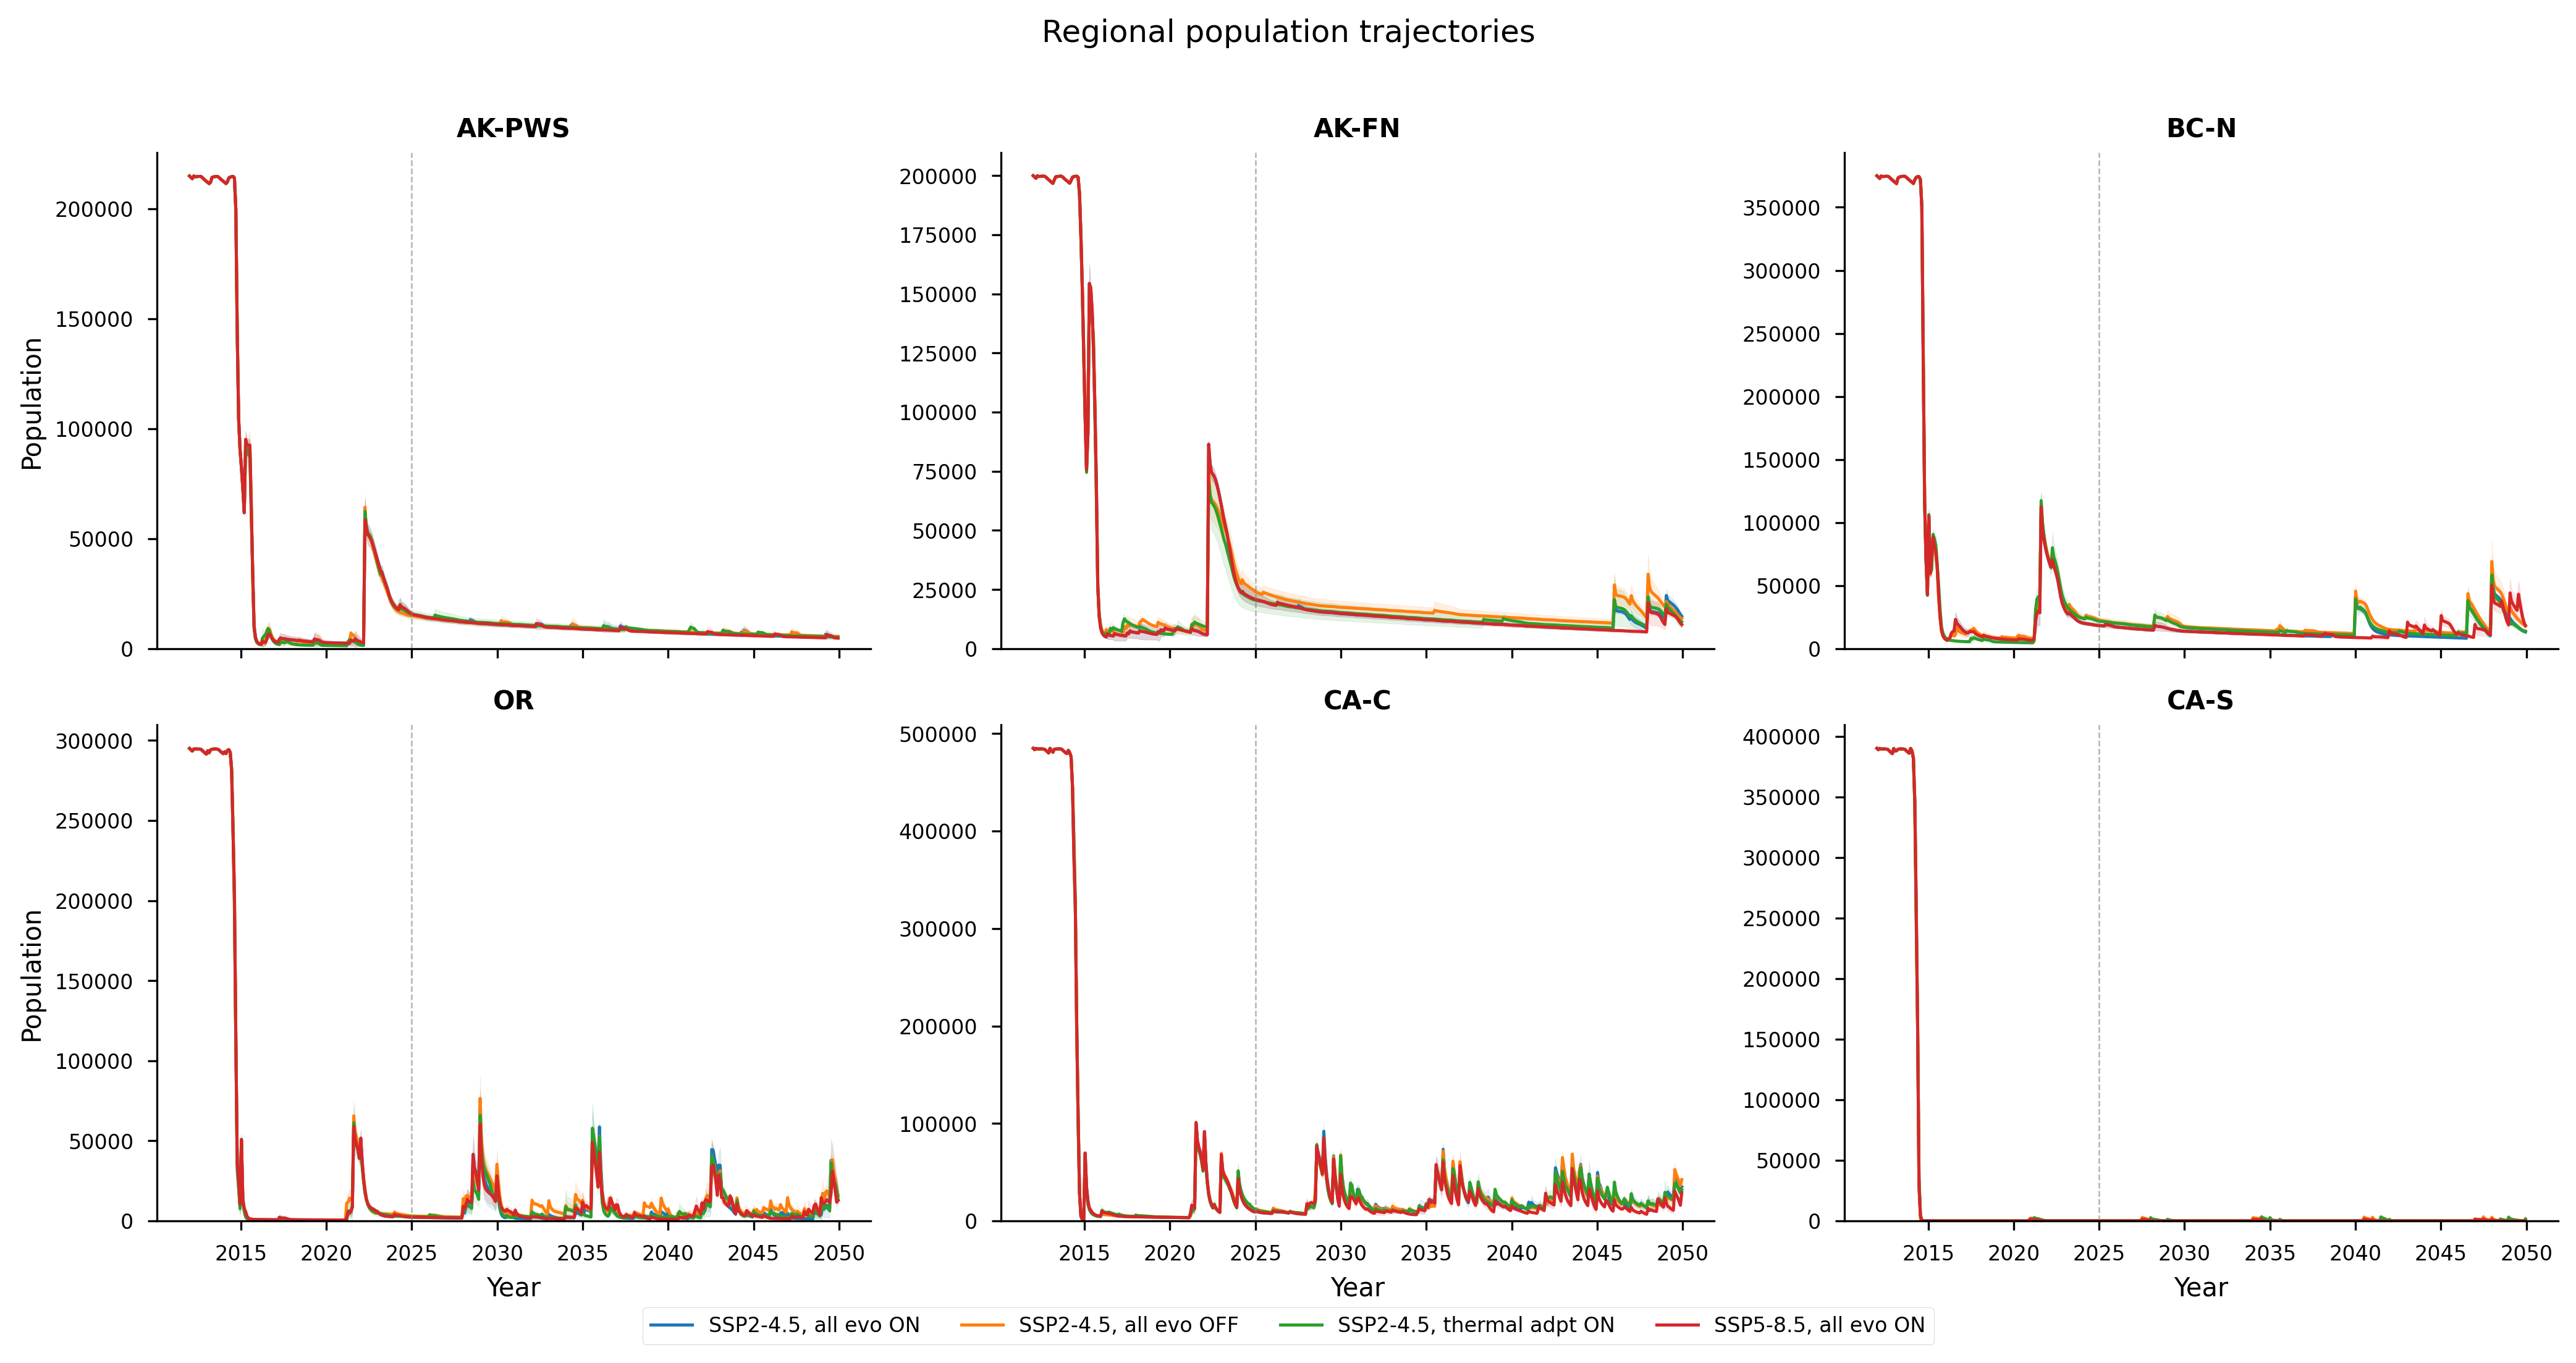
\includegraphics[width=\textwidth]{figures/fig_regional_trajectories.png}
    \caption{Population trajectories for six representative regions under all four scenarios. \textbf{Top row:} Alaska (AK-PWS, AK-FN) and British Columbia (BC-N), showing seasonal population cycling driven by winter pathogen dormancy and summer reactivation. \textbf{Bottom row:} Oregon (OR), central California (CA-C), and southern California (CA-S). Oregon sustains the highest long-term abundance; CA-S declines to extinction in all scenarios. Lines show three-seed means; shaded regions show $\pm$1 standard deviation.}
    \label{fig:regional_trajectories}
\end{figure}

In contrast, southern populations (California, Baja California) exhibit
monotonic decline with minimal seasonal modulation.  Year-round warm
SSTs in these regions maintain chronic pathogen activity, leaving
populations no seasonal refuge.  The result is a relentless erosion of
abundance that, in the most southerly regions, proceeds to functional
or absolute extinction (Section~\ref{sec:regional}).

% --- Figure: Regional Trajectories ---
\begin{figure}[!htbp]
    \centering
    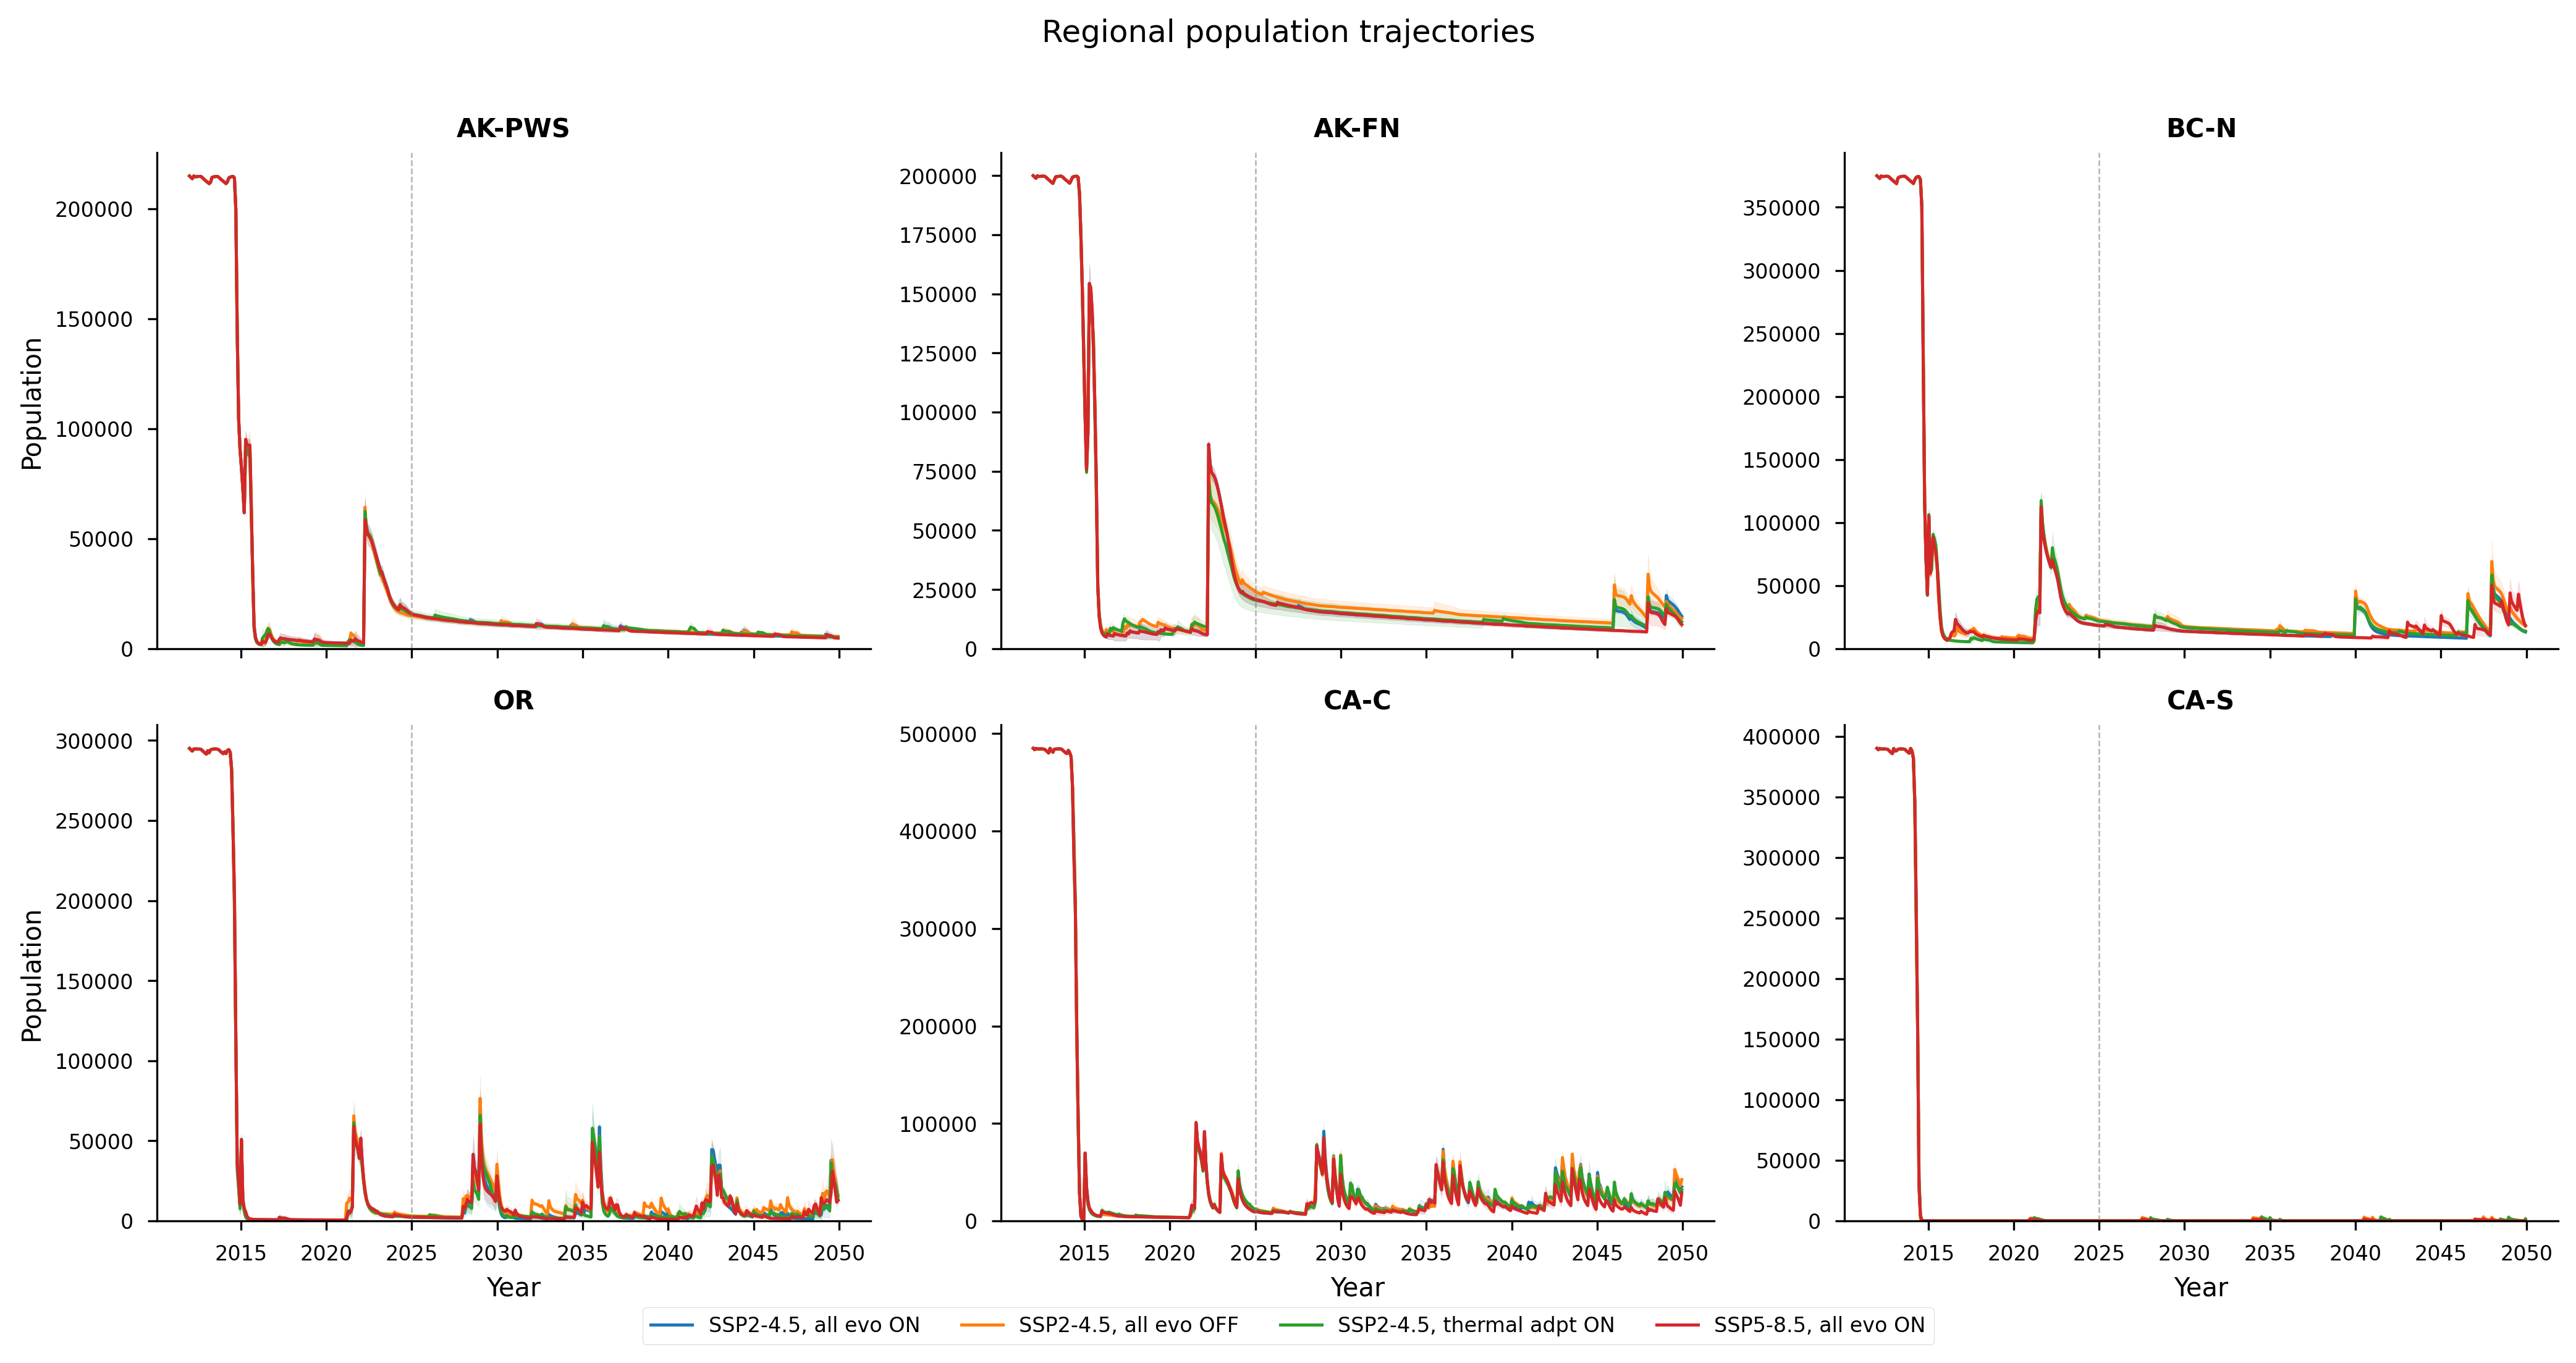
\includegraphics[width=\textwidth]{figures/fig_regional_trajectories.png}
    \caption{Population trajectories for six representative regions under all four scenarios. \textbf{Top row:} Alaska (AK-PWS, AK-FN) and British Columbia (BC-N), showing seasonal population cycling driven by winter pathogen dormancy and summer reactivation. \textbf{Bottom row:} Oregon (OR), central California (CA-C), and southern California (CA-S). Oregon shows episodic oasis dynamics with boom-bust cycles; CA-S declines to extinction in all scenarios. Lines show three-seed means; shaded regions show $\pm$1 standard deviation.}
    \label{fig:regional_trajectories}
\end{figure>

\subsubsection{The Recruitment Pulse Phenomenon}

A conspicuous feature of the simulated trajectories is the recurrence
of recruitment pulses---brief (2--6 month) surges in abundance that
interrupt the long-term decline.  These pulses arise when a sequence of
cooler-than-average months suppresses pathogen activity long enough for
surviving adults to reproduce and juveniles to recruit into the
population.  However, the pulses are inherently self-limiting: the
temporary increase in host density raises the effective contact rate,
and the subsequent return to warmer conditions triggers renewed
epizootic mortality that rapidly erases the demographic gain.

This dynamic is most pronounced in the mid-latitude transitional zone
(Washington, Oregon), where interannual SST variability is high and
the population teeters near the pathogen's thermal activation boundary.
In Alaska, pulses are smaller in amplitude but more regularly spaced,
tracking the predictable annual thermal cycle.  In southern California
and Baja, recruitment pulses are largely absent by the 2030s, as
chronic pathogen pressure suppresses reproduction below replacement
(Figure~\ref{fig:heatmap_population}).

% --- Figure: Population Heatmap ---
\begin{figure}[!htbp]
    \centering
    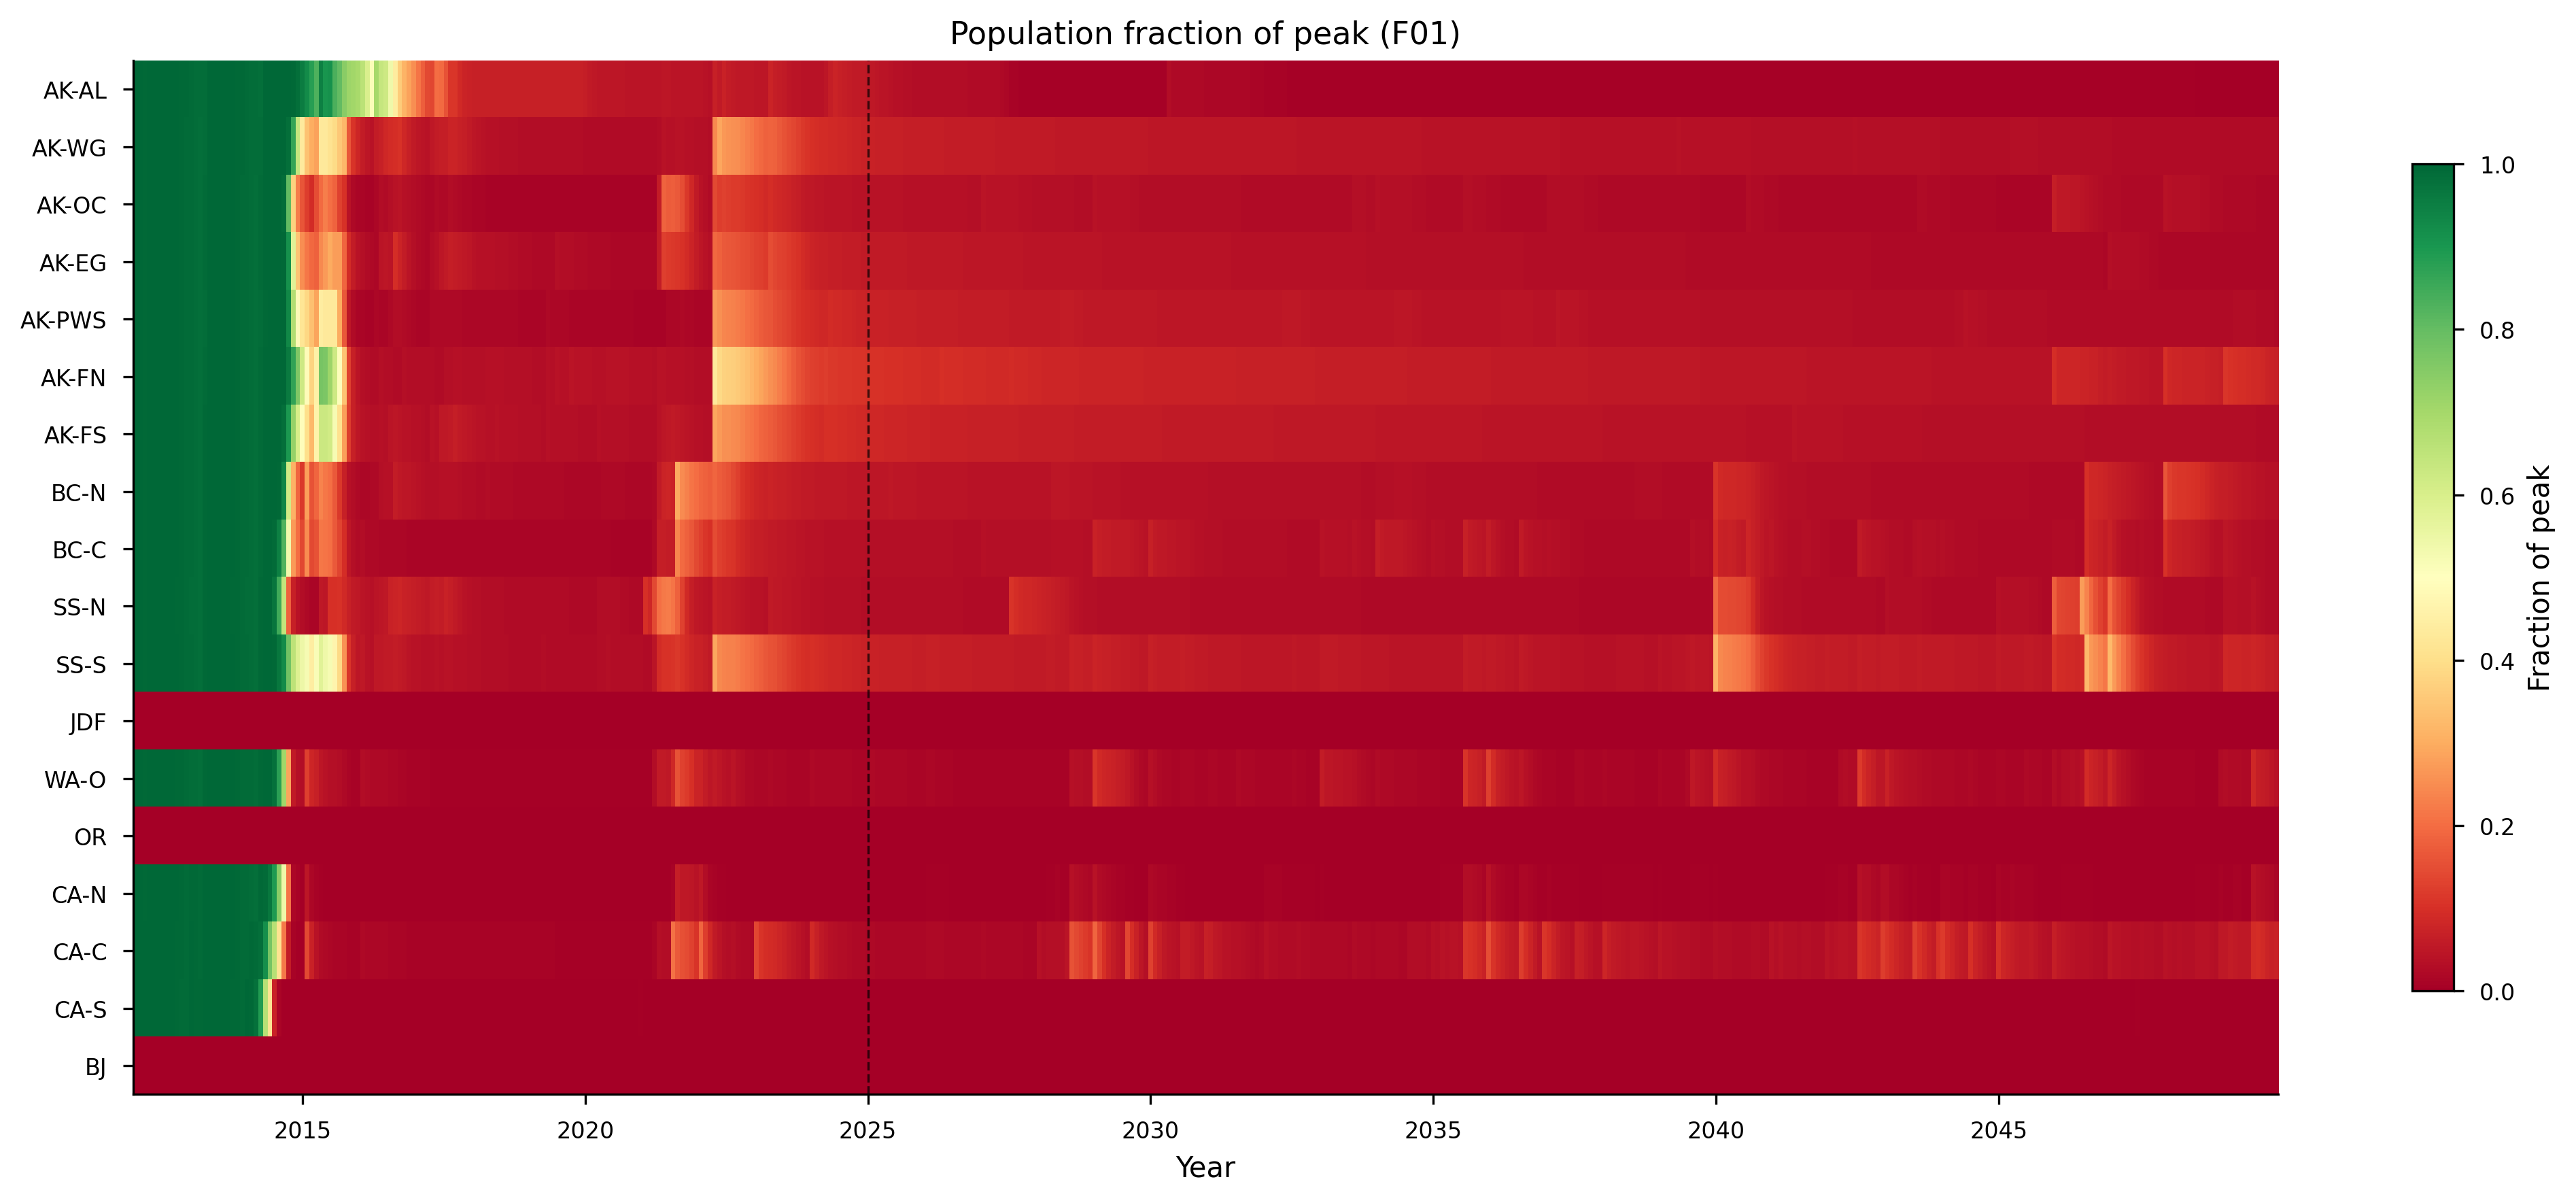
\includegraphics[width=\textwidth]{figures/fig_heatmap_population.png}
    \caption{Space--time heatmap of \textit{Pycnopodia} populations across the species' range under the baseline scenario (F01). Each row represents one of the 18 geographic regions (ordered south to north from bottom to top); the x-axis spans 2012--2050; color intensity indicates the fraction of carrying capacity occupied. The disease wavefront is visible as a dark band sweeping from south to north during 2013--2015. Post-crash, southern regions (BJ, CA-S) remain permanently dark (extinct), while a few northern and mid-latitude regions retain pale coloration (partial persistence). The 2025 observation-to-projection transition is marked.}
    \label{fig:heatmap_population}
\end{figure>

% ---------------------------------------------------------------------------
\subsection{Regional Recovery Patterns}
\label{sec:regional}

Table~\ref{tab:regional} presents the full matrix of regional recovery
percentages (surviving population as a fraction of initial abundance)
across all 18 model regions and four scenarios.

\begin{table}[htbp]
\centering
\caption{Regional recovery at 2050 (\% of initial population
surviving), grouped by geographic cluster.  Values are three-seed means.
Bold values indicate the highest recovery within each region across
scenarios. Note: Oregon's 17.6\% value represents an endpoint artifact; 
the 5-year average (2045--2050) is 5.4\% due to extreme boom-bust cycles.}
\label{tab:regional}
\smallskip
\small
\begin{tabular}{ll rrrr}
\toprule
\textbf{Cluster} & \textbf{Region} & \textbf{F01} & \textbf{F02} &
  \textbf{F03} & \textbf{F04} \\
\midrule
\multirow{7}{*}{\rotatebox[origin=c]{90}{\textbf{Alaska}}}
 & AK-AL  &  0.4 & \textbf{4.1} &  0.7 &  0.4 \\
 & AK-WG  &  2.5 & \textbf{4.5} &  3.0 &  2.4 \\
 & AK-OC  &  1.8 &  3.1          &  1.5 & \textbf{6.0} \\
 & AK-EG  &  1.7 & \textbf{2.4} &  2.0 &  1.6 \\
 & AK-PWS &  2.4 & \textbf{2.6} &  2.5 &  2.2 \\
 & AK-FN  &  6.8 &  6.4          &  5.7 & \textbf{9.9} \\
 & AK-FS  &  2.7 &  3.6          &  2.9 & \textbf{10.3} \\
\midrule
\multirow{4}{*}{\rotatebox[origin=c]{90}{\textbf{BC/SS}}}
 & BC-N   &  3.6 &  4.9          &  3.7 & \textbf{11.3} \\
 & BC-C   &  3.3 & \textbf{7.5} &  4.1 &  6.4 \\
 & SS-N   &  2.4 & \textbf{3.6} &  2.6 &  3.1 \\
 & SS-S   &  6.5 & \textbf{8.8} &  7.7 &  7.6 \\
\midrule
\multirow{3}{*}{\rotatebox[origin=c]{90}{\textbf{PNW}}}
 & JDF    &  5.4 & \textbf{6.5} &  5.9 &  5.3 \\
 & WA-O   & \textbf{8.8} &  5.1 &  4.2 &  6.0 \\
 & OR     & \textbf{17.6} & 12.8 & 15.3 & 10.4 \\
\midrule
\multirow{4}{*}{\rotatebox[origin=c]{90}{\textbf{CA/BJ}}}
 & CA-N   &  5.0 & \textbf{5.9} &  2.9 &  4.3 \\
 & CA-C   & \textbf{11.9} & 11.9 & 11.5 &  7.6 \\
 & CA-S   &  0.0 &  0.1          & \textbf{0.4} &  0.0 \\
 & BJ     &  0.0 &  0.0          &  0.0 &  0.0 \\
\bottomrule
\end{tabular}
\end{table}

\subsubsection{Alaska}

Alaskan populations uniformly show poor recovery across all scenarios,
with most regions retaining fewer than 3\% of initial abundance under
the baseline (F01).  The exception is AK-FN (Funter Bay--northern
Southeast Alaska), which achieves 6.8\% under F01 and reaches 9.9\%
under the high-warming scenario F04.  The consistently low values
throughout western and south-central Alaska reflect the combination of
cold winters that limit the reproductive season and summers that,
despite being cool by lower-latitude standards, are now warm enough to
sustain episodic pathogen outbreaks.

Notably, several Alaskan regions show their strongest recovery under
F04 (SSP5-8.5), particularly AK-FS (+7.6 percentage points relative to
F01) and AK-OC (+4.2 points).  This counterintuitive result---warming
\textit{helping} northern populations---is discussed in
Section~\ref{sec:climate_effects}.

\subsubsection{British Columbia and the Salish Sea}

British Columbia and the Salish Sea region display moderate recovery
potential (3--9\%) with substantial sensitivity to both climate and
evolutionary scenarios.  BC-N (northern British Columbia) is among the
most climate-responsive regions in the entire domain, increasing from
3.6\% under F01 to 11.3\% under F04---a gain of 7.7 percentage
points that makes it the single largest beneficiary of high-end warming
(Figure~\ref{fig:regional_recovery_bars}).  BC-C (central British
Columbia) is instead most sensitive to pathogen evolution, jumping from
3.3\% (F01) to 7.5\% (F02, evolution off), a gain of 4.2 points.

The Salish Sea subregions (SS-N, SS-S) exhibit intermediate recovery
and moderate scenario sensitivity.  SS-S consistently outperforms SS-N,
likely reflecting the greater habitat complexity and cooler deep-water
refugia of the southern basins.

\subsubsection{Pacific Northwest: Oregon's Episodic Dynamics}

The Pacific Northwest cluster reveals the most striking regional
pattern in the entire forecast ensemble.  Oregon (OR) appears to be 
the recovery leader in 2050 endpoint snapshots (17.6\%), but this 
reflects boom-bust episodic dynamics rather than sustained recovery. 
Oregon's 5-year average (2045--2050) is 5.4\% with 121\% coefficient 
of variation, indicating extreme volatility. Alaska's Fairweather-North 
region shows more reliable persistence (6.8\% snapshot, 9.4\% 5-year 
average). Oregon's episodic advantage derives from oasis sites that 
periodically boom due to strong upwelling, thermal variability, and 
sweepstakes reproductive success, but these gains are repeatedly erased 
by subsequent pathogen activity.

However, Oregon's episodic dynamics are also highly vulnerable to both 
warming and evolutionary change.  Under F04 (high warming), Oregon's 
endpoint snapshot drops to 10.4\%---a loss of 7.2 percentage points 
affecting both snapshots and underlying averages, the largest negative
climate effect of any region.  Under F02 (no evolution), Oregon's 
endpoint declines to 12.8\%, losing 4.8 points despite the coast-wide 
benefit of freezing pathogen evolution.  These paradoxical vulnerabilities 
reflect the fragility of Oregon's oasis-driven boom-bust cycles and are
analyzed in Sections~\ref{sec:climate_effects} and \ref{sec:pathogen_evo}.

Outer Washington (WA-O) follows a distinctive pattern, achieving its
highest recovery (8.8\%) under F01 but declining under all alternative
scenarios---including F02, where disabling pathogen evolution actually
reduces its recovery by 3.7 percentage points.

\subsubsection{California and Baja California: Southern Collapse}

Southern California (CA-S) and Baja California (BJ) are functionally
extinct across all scenarios.  CA-S retains at most 0.4\% of its
initial population (under F03), while BJ achieves 0.0\% in every
scenario.  These results indicate that even under moderate warming with
favorable evolutionary assumptions, the southern range limit of
\textit{P.~helianthoides} has contracted northward past approximately
33\textdegree N and is unlikely to recover within the forecast horizon.

Central California (CA-C) presents a more nuanced picture: it maintains
robust recovery (11.9\%) under both F01 and F02 but declines
substantially (to 7.6\%) under high warming (F04).  Northern California
(CA-N) is intermediate, with moderate recovery (5.0--5.9\%) under
SSP2-4.5 scenarios but reduced persistence (4.3\%) under SSP5-8.5.

The extinction of southern populations represents the loss of a
significant fraction of the species' historical genetic diversity and
raises conservation concerns that extend beyond simple abundance
metrics (Section~\ref{sec:evo_dynamics}).

% ---------------------------------------------------------------------------
\subsection{Climate Effects}
\label{sec:climate_effects}

The contrast between F01 (SSP2-4.5) and F04 (SSP5-8.5), both with
full evolutionary dynamics, isolates the effect of enhanced ocean
warming on population outcomes.  Coast-wide, the net effect is
remarkably small: F04 retains 5.8\% of the initial population versus
5.4\% under F01, a difference of only +0.4 percentage points.  This
near-zero aggregate effect, however, masks a dramatic latitudinal
redistribution of surviving populations
(Figure~\ref{fig:climate_effect}).

\subsubsection{Northern Beneficiaries}

The largest positive climate effects are concentrated in a band from
southern Alaska through northern British Columbia
(Figure~\ref{fig:recovery_vs_latitude}):

% --- Figure: Recovery vs Latitude ---
\begin{figure}[!htbp]
    \centering
    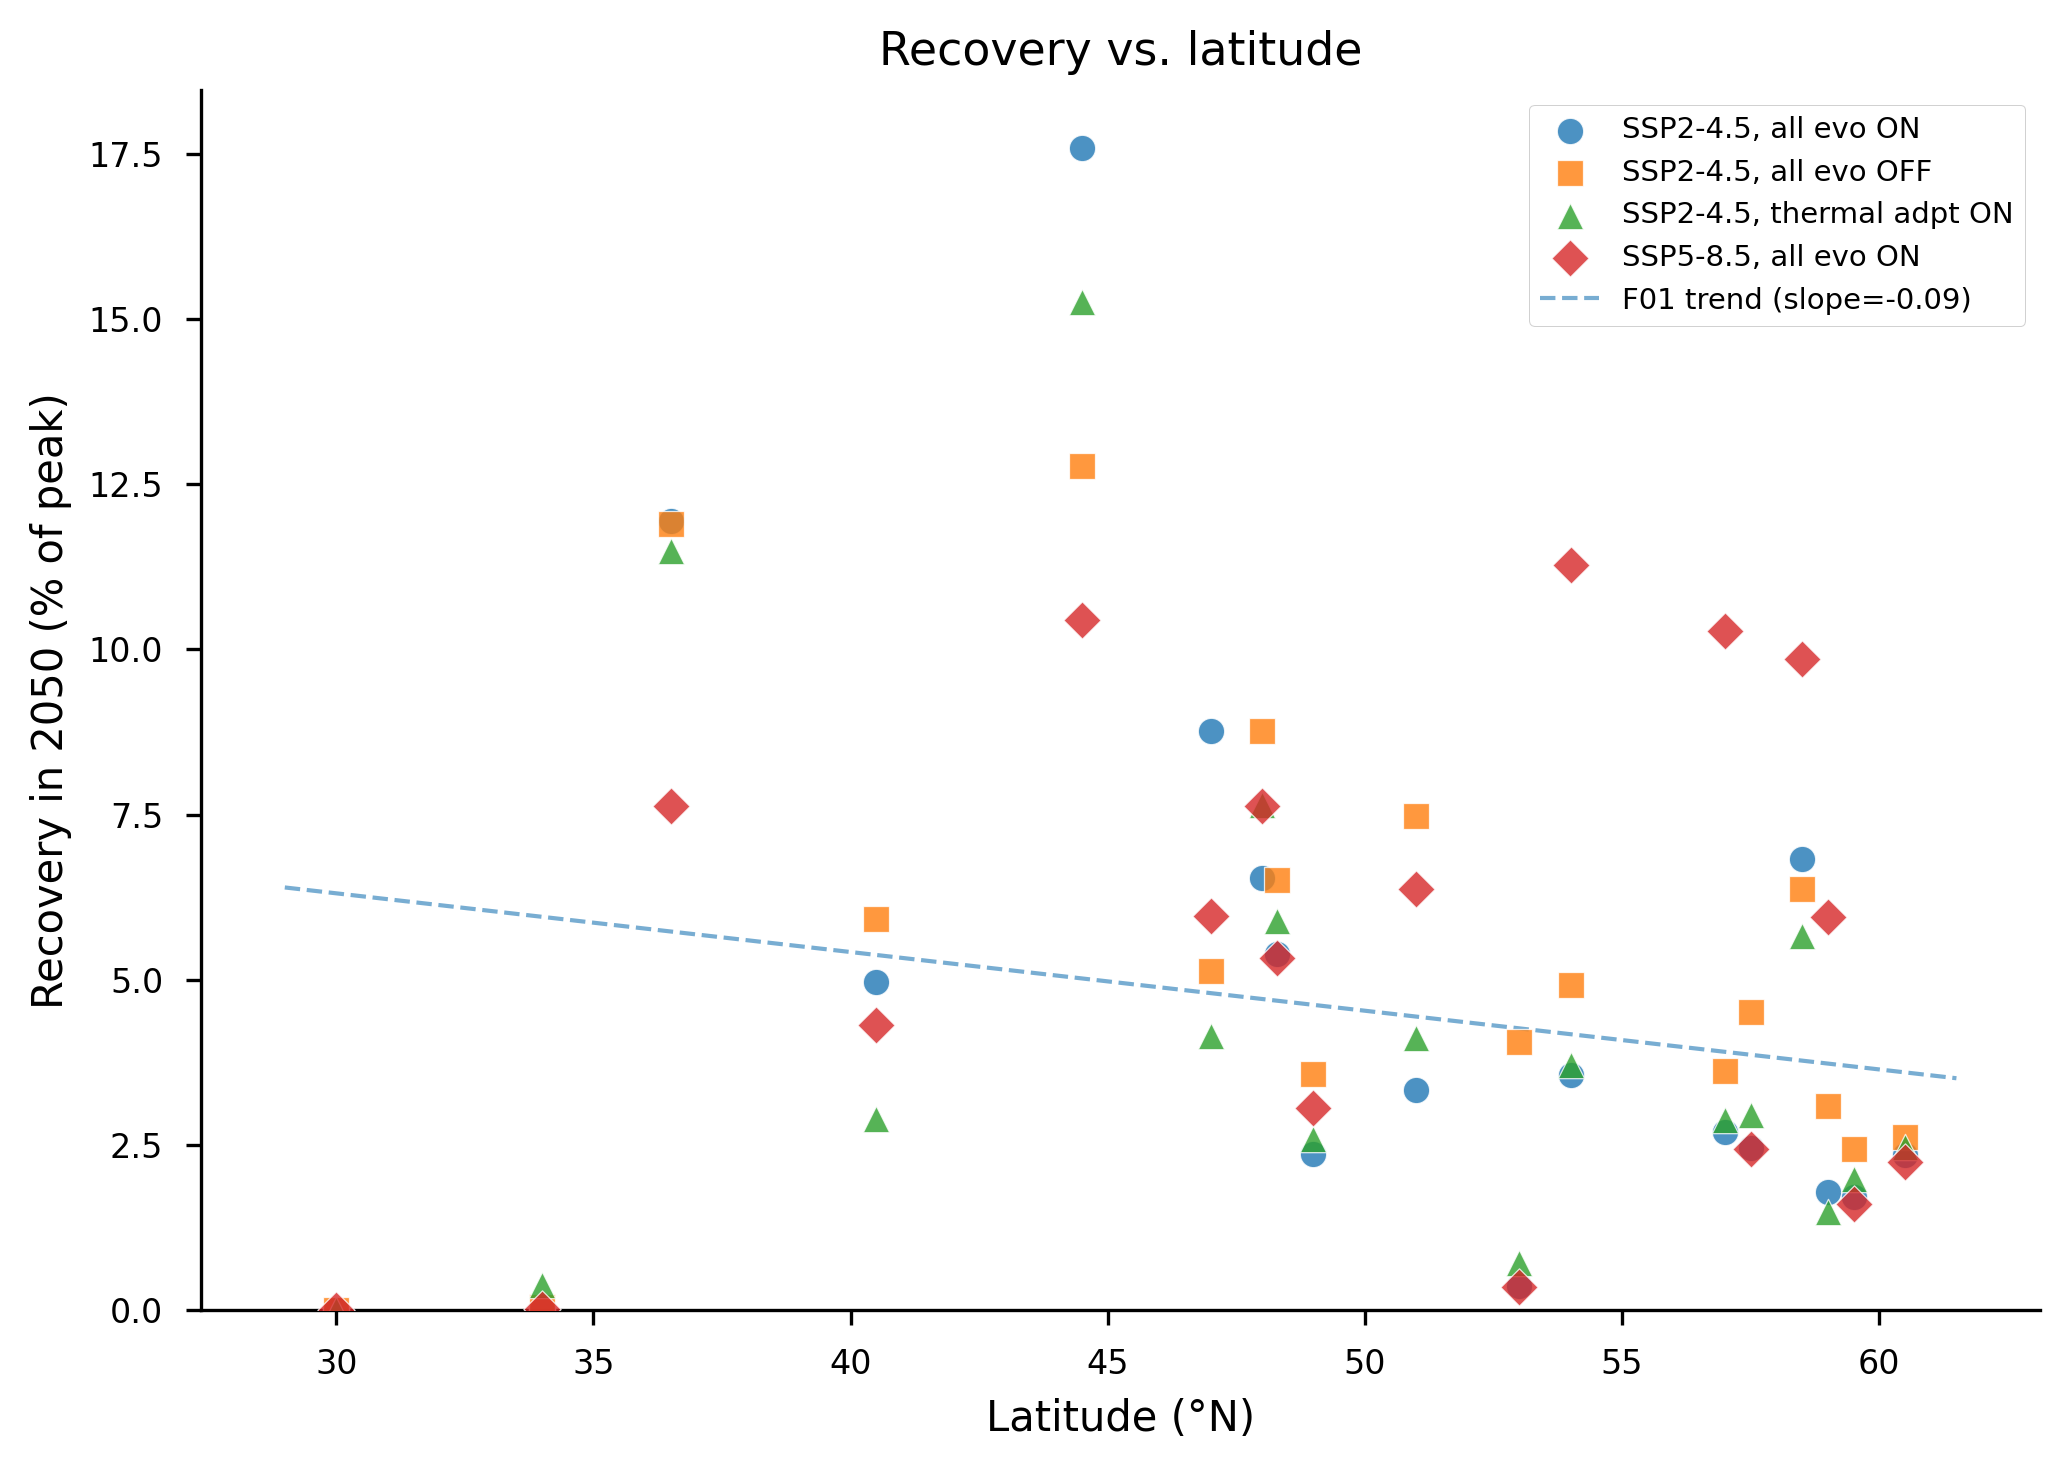
\includegraphics[width=0.75\textwidth]{figures/fig_recovery_vs_latitude.png}
    \caption{Recovery fraction vs.\ latitude for all 18 regions across four scenarios. Each point represents a region's three-seed mean recovery percentage at 2050. Under baseline conditions (F01, blue), Oregon ($\sim$45\textdegree N) shows a 2050 endpoint artifact of 17.6\% (5-year average: 5.4\% with high variability), while Alaska's Fairweather-North provides more reliable recovery. Under high warming (F04, red), the high-latitude tail lifts substantially while the mid-latitude peak flattens, reflecting the northward shift in favorable conditions. The relationship between latitude and recovery is nonlinear and non-monotonic, driven by the interplay of temperature-dependent pathogen activity, host reproductive season length, and site-specific hydrodynamic flushing.}
    \label{fig:recovery_vs_latitude}
\end{figure>

\begin{itemize}
  \item BC-N: $+$7.7 percentage points (3.6\% $\rightarrow$ 11.3\%)
  \item AK-FS: $+$7.6 points (2.7\% $\rightarrow$ 10.3\%)
  \item AK-OC: $+$4.2 points (1.8\% $\rightarrow$ 6.0\%)
  \item AK-FN: $+$3.1 points (6.8\% $\rightarrow$ 9.9\%)
  \item BC-C: $+$3.1 points (3.3\% $\rightarrow$ 6.4\%)
\end{itemize}

\noindent
The mechanism underlying this northern benefit operates through two
complementary pathways.  First, warming extends the effective growing
season for \textit{P.~helianthoides} at high latitudes, where
cold-limited reproduction constrains population growth rates more
severely than disease-induced mortality during most of the year.
Second, although warming also extends the pathogen's active season,
the absolute SSTs in these regions remain near the lower boundary of
the pathogen's thermal niche even under SSP5-8.5, limiting the
intensity and duration of summer epizootics.  The net balance thus
favors the host: more reproduction in spring and autumn, with only
modestly increased disease pressure in summer.

\subsubsection{Southern Losers}

South of approximately 48\textdegree N, warming uniformly depresses
recovery:

\begin{itemize}
  \item OR: $-$7.2 percentage points (17.6\% $\rightarrow$ 10.4\%)
  \item CA-C: $-$4.3 points (11.9\% $\rightarrow$ 7.6\%)
  \item WA-O: $-$2.8 points (8.8\% $\rightarrow$ 6.0\%)
  \item CA-N: $-$0.7 points (5.0\% $\rightarrow$ 4.3\%)
\end{itemize}

\noindent
In these regions, baseline SSTs are already warm enough to sustain
prolonged pathogen activity.  Additional warming expands the window of
active transmission into what were previously marginal shoulder
seasons, increasing the cumulative annual disease burden.
Simultaneously, these populations are already near the upper thermal
tolerance for reproduction, so warming provides little compensatory
demographic benefit.  Oregon suffers the steepest absolute decline
because it has the most to lose: its high baseline recovery rate
amplifies the proportional impact of extended pathogen activity seasons.

\subsubsection{The Breakeven Latitude}

The transition from net climate benefit (north) to net climate cost
(south) occurs at approximately 48\textdegree N---roughly the latitude
of the Juan de Fuca Strait and the boundary between the
upwelling-dominated California Current system and the downwelling
regime of the northern shelf.  This breakeven latitude is not merely a
statistical artifact but reflects a genuine biophysical boundary: north
of 48\textdegree N, winter SSTs are sufficiently cold that the pathogen
enters prolonged VBNC dormancy, and warming's primary effect is to
accelerate host population growth during the expanded ice-free season.
South of this boundary, the pathogen's dormancy period is already short
or absent, and warming's primary effect is to intensify chronic disease
pressure.

The existence of this breakeven latitude has important conservation
implications.  Under high-end warming, the center of abundance for
\textit{P.~helianthoides} shifts northward by several degrees of
latitude, with northern British Columbia and southeastern Alaska
emerging as the primary refugia.  This geographic shift could alter the
species' ecological role along the coast, as regions that currently
benefit from sunflower star predation on sea urchins (notably the
California kelp forests) would lose this keystone function while
regions with less acute urchin overgrazing pressure gain it.

% ---------------------------------------------------------------------------
\subsection{Evolutionary Dynamics}
\label{sec:evo_dynamics}

The coupled eco-evolutionary framework tracks the temporal evolution of
both host resistance and pathogen traits at each of the 896 model
sites.  Under the baseline scenario (F01), these traits exhibit
striking spatial gradients and temporal dynamics that illuminate the
interplay between selection, drift, and demographic constraint.

\subsubsection{Host Resistance}

Mean host resistance ($\bar{r}$) increases from the uniform initial
value of 0.150 toward higher values in all surviving populations, but
the rate and ultimate level of resistance evolution vary enormously
across the latitudinal range
(Figure~\ref{fig:resistance_evolution}):

\begin{itemize}
  \item \textbf{Alaska (moderate selection, slow response):}
    AK-PWS: $0.150 \rightarrow 0.253$;
    AK-FN: $0.150 \rightarrow 0.230$.
    Disease pressure is seasonal and moderate, producing
    consistent but gentle directional selection.
  \item \textbf{British Columbia (intermediate):}
    BC-N: $0.150 \rightarrow 0.240$.
    Stronger summer epizootics drive faster allele frequency
    change than in Alaska, but demographic stability maintains
    sufficient population sizes for effective selection.
  \item \textbf{Oregon and California (intense selection, rapid
    response):}
    OR: $0.150 \rightarrow 0.378$;
    CA-C: $0.150 \rightarrow 0.425$.
    Year-round pathogen activity imposes sustained, intense
    selection for resistance.  CA-C achieves the highest
    resistance of any surviving population, with mean $\bar{r}$
    reaching 0.43 by 2050.
  \item \textbf{Southern California (extinction):}
    CA-S: $0.150 \rightarrow 0.115$ (approximately 52 survivors).
    Mean resistance actually \textit{declines} below the starting
    value, because the population is so small (${\sim}$50 individuals)
    that genetic drift overwhelms directional selection.
\end{itemize}

\noindent
A critical observation is that even the highest evolved resistance
level ($\bar{r} = 0.425$ in CA-C) provides only partial protection:
at this resistance level, 58\% of the force of infection still
penetrates host defenses.  In the context of the model's multiplicative
disease framework, this means that CA-C populations in 2050 still
experience more than half the per-capita disease mortality of a
completely na\"ive population.  Resistance evolution slows the decline
but does not arrest it.

\subsubsection{The Cruel Paradox of Evolutionary Capacity}

The populations under the most intense selection for resistance are
precisely those with the least capacity to respond.  In southern
populations, chronic pathogen pressure drives rapid allele frequency
change but simultaneously erodes population size, reducing the
effective population size ($N_e$) and hence the efficiency of
selection.  As $N_e$ declines, genetic drift increasingly overwhelms
directional selection, and the additive genetic variance available for
further adaptation collapses
(Figure~\ref{fig:genetic_diversity}).

This evolutionary trap is starkest in CA-S, where the population
declines to approximately 52 individuals by 2050 despite experiencing
intense selection pressure.  Remarkably, the mean resistance of these
survivors ($\bar{r} = 0.115$) is actually \textit{lower} than the
starting value (0.150)---evidence that in such a tiny population,
genetic drift has overwhelmed directional selection.  The few surviving
individuals are not the ``most resistant''; they are simply the ones
that happened to survive through stochastic chance.  Allee effects
and demographic stochasticity now dominate their fate far more than
any genetic advantage.

The paradox generalizes across the southern range: the populations that
``need'' evolutionary rescue the most are those least likely to achieve
it, because the disease that creates the selection pressure also
destroys the demographic base required for effective evolutionary
response.  This result echoes theoretical predictions from
evolutionary rescue theory \citep{gomulkiewicz1995, bell2008} and
provides a concrete, spatially explicit demonstration of its
consequences for a real species undergoing an ongoing epizootic.

% --- Figure: Genetic Diversity ---
\begin{figure}[!htbp]
    \centering
    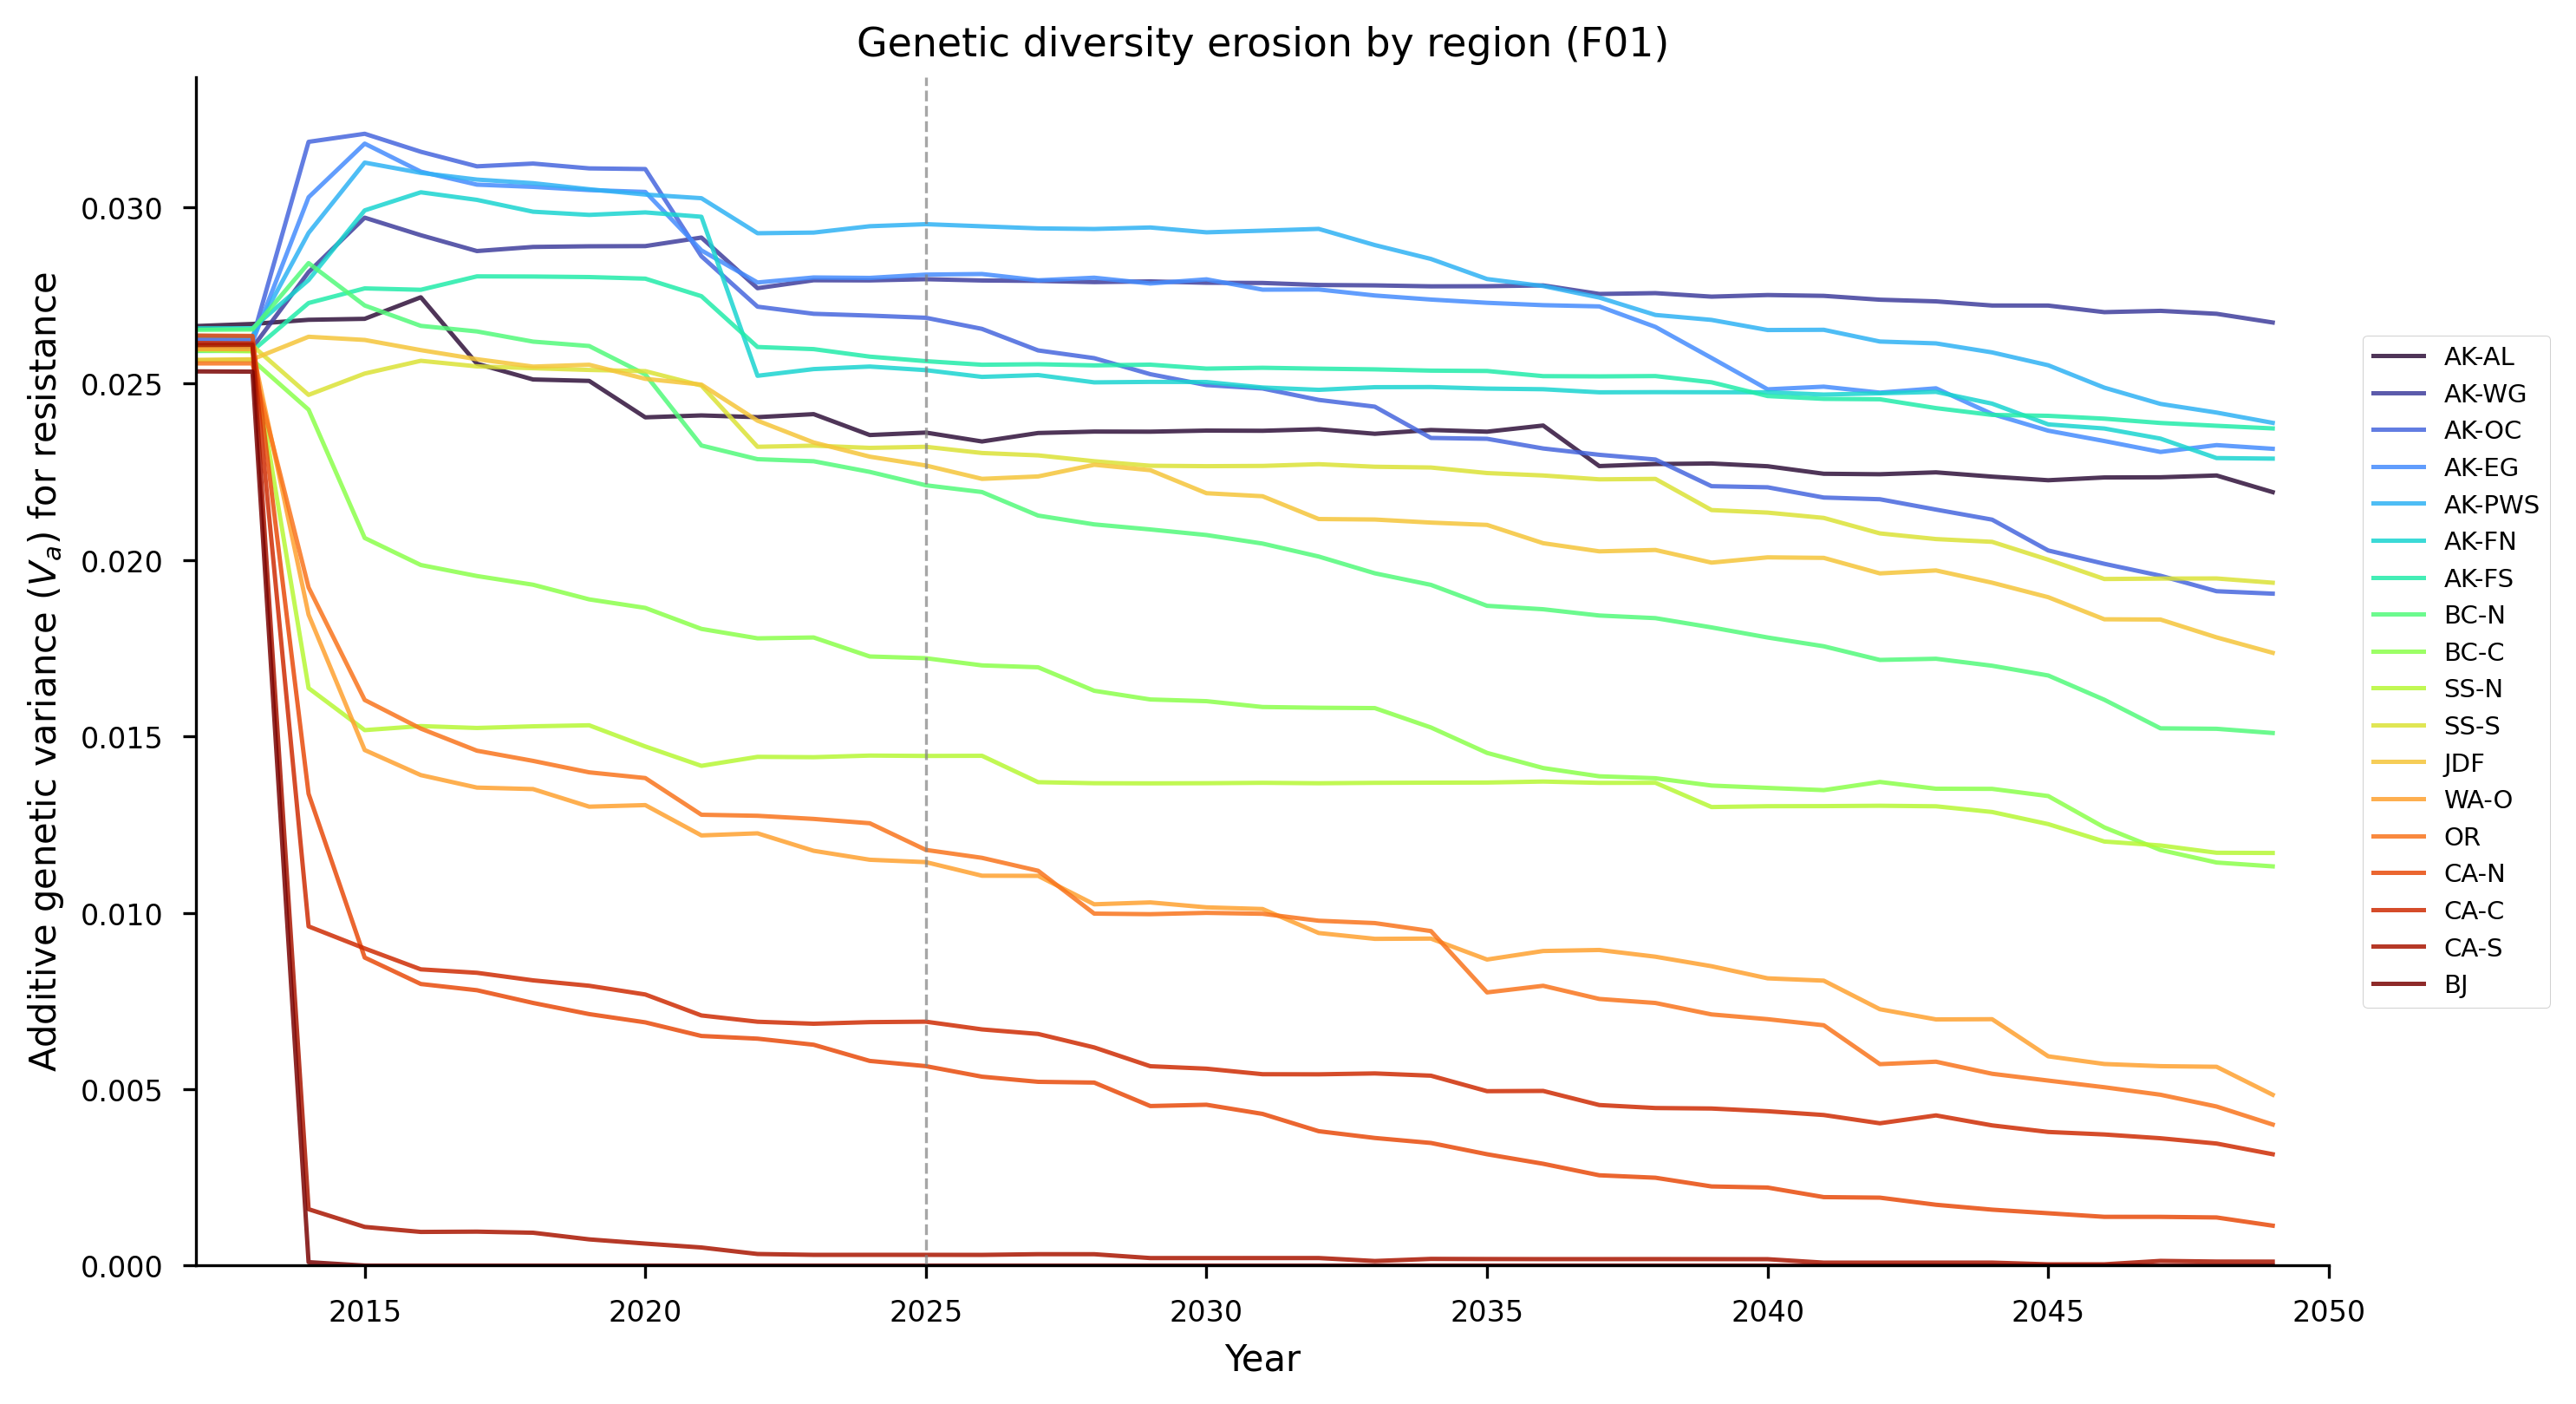
\includegraphics[width=0.75\textwidth]{figures/fig_genetic_diversity.png}
    \caption{Additive genetic variance ($V_A$) for the resistance trait across six regions under the baseline scenario (F01). $V_A$ measures the raw material available for future evolutionary adaptation. Southern populations (CA-C, CA-S) lose genetic diversity rapidly as intense disease selection eliminates most genotypes. By 2050, CA-C retains only a fraction of its initial $V_A$---the population has evolved substantially but is running out of ``evolutionary fuel.' Northern populations (AK-PWS, AK-FN) maintain higher $V_A$ because weaker selection preserves more genotypic diversity. This creates a cruel paradox: the populations that most need to evolve have the least remaining capacity to do so.}
    \label{fig:genetic_diversity}
\end{figure}

\subsubsection{Pathogen Thermal Adaptation}

The pathogen's VBNC threshold temperature ($T_\mathrm{vbnc}$)---the
SST below which the pathogen enters dormancy---evolves toward lower
values in cold-water regions as strains with broader thermal niches
gain a fitness advantage through extended transmission seasons.  By
2050 under F01, $T_\mathrm{vbnc}$ has declined to its implemented
lower bound of 9.00\textdegree C throughout Alaska (AK-PWS:
9.00\textdegree C; AK-FN: 9.00\textdegree C), indicating that
selection has driven the trait to the edge of the modeled parameter
space within 38 years (Figure~\ref{fig:pathogen_traits}).

% --- Figure: Pathogen Traits ---
\begin{figure}[!htbp]
    \centering
    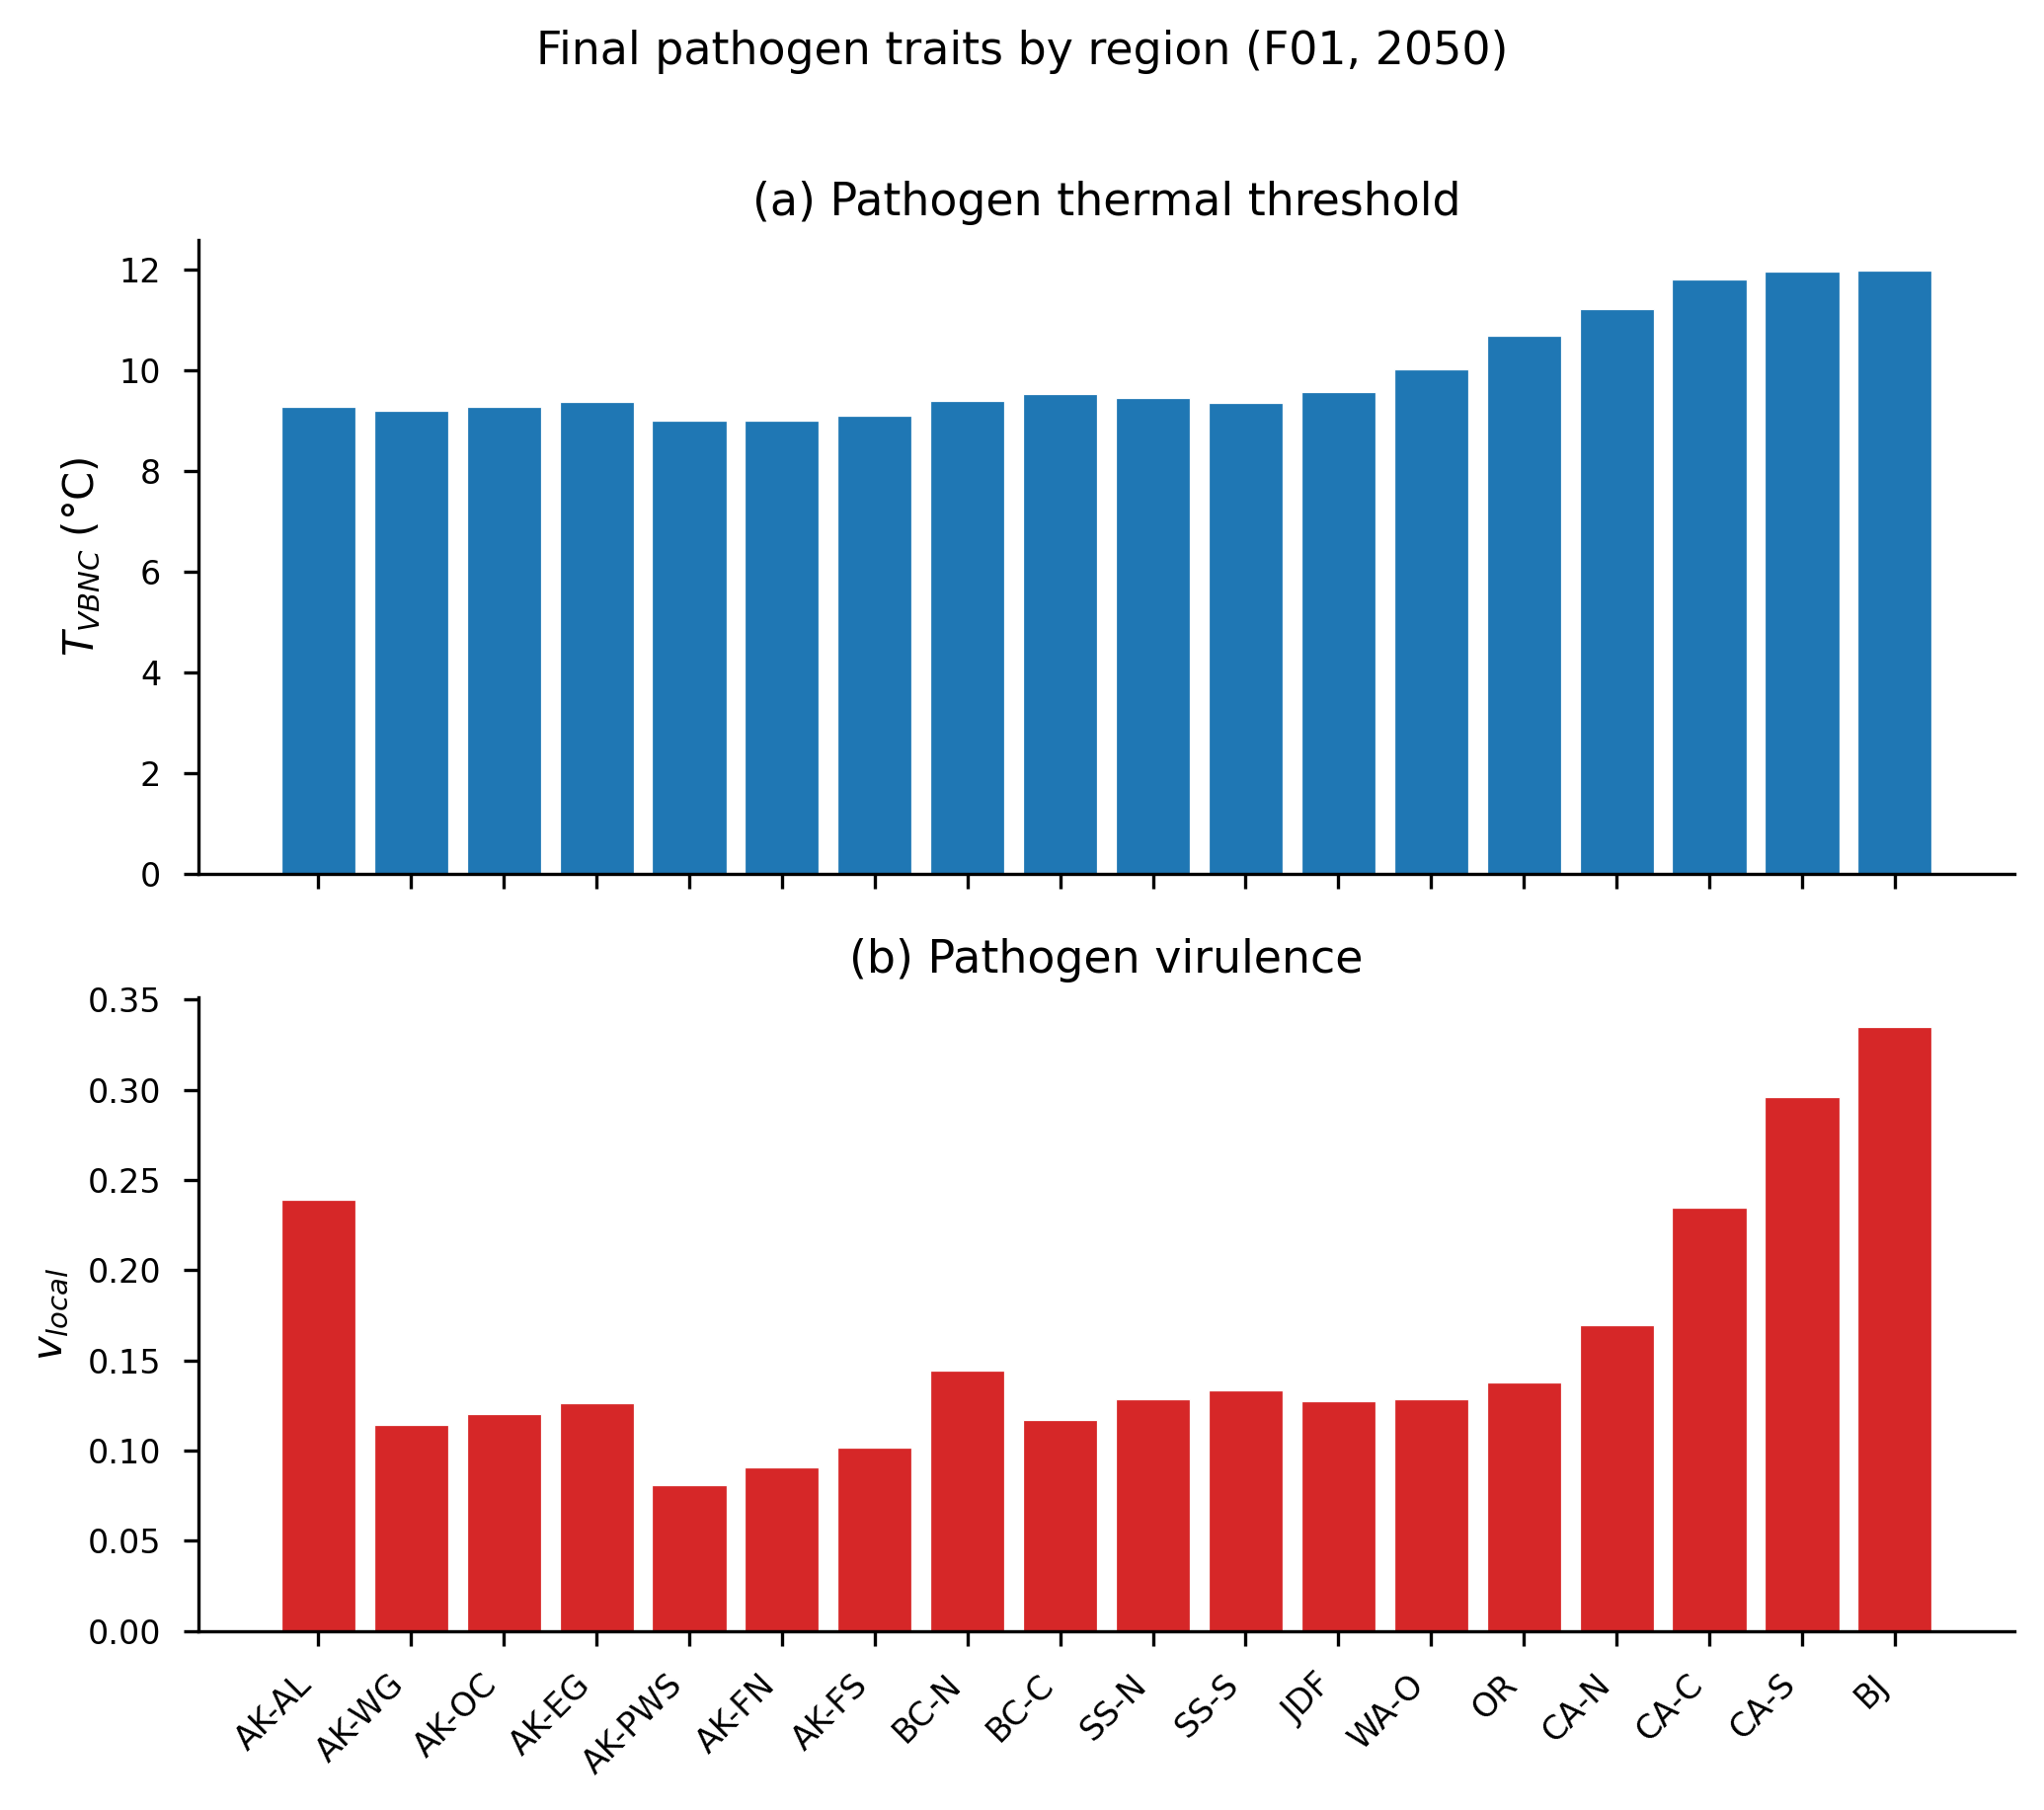
\includegraphics[width=0.75\textwidth]{figures/fig_pathogen_traits_final.png}
    \caption{Final (2050) pathogen community traits across all 18 regions under the baseline scenario (F01). \textbf{Top:} Thermal activation threshold ($T_{\text{vbnc}}$), showing how northern pathogen communities have evolved to activate at lower temperatures (reaching the 9\textdegree C biophysical floor throughout Alaska), while southern communities remain near the initial 12\textdegree C. \textbf{Bottom:} Local virulence ($v_{\text{local}}$), showing the latitudinal gradient predicted by virulence--transmission trade-off theory: high virulence in warm, dense southern waters (Baja: 0.34) and low virulence in cold, sparse northern waters (Alaska: 0.09).}
    \label{fig:pathogen_traits}
\end{figure>

At lower latitudes, $T_\mathrm{vbnc}$ settles at intermediate values
that reflect a balance between selection for broader thermal niches and
the diminishing marginal fitness return of further thermal adaptation
in already-warm environments:

\begin{itemize}
  \item BC-N: $T_\mathrm{vbnc} = 9.39$\textdegree C
  \item OR: $T_\mathrm{vbnc} = 10.70$\textdegree C
  \item CA-C: $T_\mathrm{vbnc} = 11.81$\textdegree C
  \item BJ: $T_\mathrm{vbnc} = 12.00$\textdegree C (upper bound,
    unchanged from initialization)
\end{itemize}

\noindent
The latitudinal gradient in $T_\mathrm{vbnc}$ is opposite to what
might na\"ively be expected.  In warm regions, the pathogen has no
``need'' to adapt its thermal niche because ambient temperatures
already exceed activation thresholds year-round; consequently,
$T_\mathrm{vbnc}$ remains near its initial value.  In cold regions,
even small reductions in $T_\mathrm{vbnc}$ substantially extend the
annual transmission window, creating strong selection for thermal
generalism.

The saturation of $T_\mathrm{vbnc}$ at 9.00\textdegree C throughout
Alaska by 2050 implies that pathogen thermal adaptation has effectively
reached its maximum extent in the north within the modeled range.
Further increases in pathogen pressure at high latitudes would require
either warming of SSTs above the adapted threshold for longer periods
or evolution of $T_\mathrm{vbnc}$ below the 9\textdegree C floor---a
possibility our model does not permit but that merits investigation in
future work.

\subsubsection{Virulence Gradient}

Local virulence ($v_\mathrm{local}$) evolves independently at each
site, driven by the interplay between within-host selection for
increased pathogen replication and the epidemiological cost of host
mortality.  By 2050, a pronounced latitudinal virulence gradient has
developed (Figure~\ref{fig:pathogen_traits}):

\begin{center}
\begin{tabular}{lc}
\toprule
\textbf{Region} & $v_\mathrm{local}$ (2050) \\
\midrule
AK-PWS & 0.081 \\
AK-FN  & 0.091 \\
BC-N   & 0.144 \\
OR     & 0.138 \\
CA-C   & 0.235 \\
BJ     & 0.335 \\
\bottomrule
\end{tabular}
\end{center}

\noindent
Virulence increases fourfold from Alaska (0.086) to Baja California
(0.343).  This gradient arises because southern populations sustain
chronic, dense pathogen populations year-round, favoring
aggressive strains that maximize short-term transmission.  In the
north, the annual interruption of transmission by winter cooling
selects against hyper-virulent strains that kill their hosts before the
next transmission season---a classic prediction of the
transmission--virulence trade-off hypothesis applied to a seasonally
structured environment \citep{alizon2009}.

The virulence gradient reinforces the north--south asymmetry already
created by climate: southern populations face not only longer pathogen
activity seasons but also intrinsically more virulent pathogen
populations, compounding the demographic disadvantage.

% ---------------------------------------------------------------------------
\subsection{The Pathogen Evolution Question}
\label{sec:pathogen_evo}

A central motivation of this study is to determine whether pathogen
evolution materially alters the long-term forecast for
\textit{P.~helianthoides}.  The factorial design permits direct
quantification of this effect through comparison of scenarios with
(F01) and without (F02) pathogen evolutionary capacity, and through the
intermediate case where only virulence evolution is disabled (F03).

\subsubsection{Aggregate Effect: Modest and Counterintuitive}

Coast-wide, disabling all pathogen evolution (F02) yields a modest
improvement: 5.9\% survival versus 5.4\% under F01, a difference of
$+$0.5 percentage points (Figure~\ref{fig:evo_comparison}).  This
result confirms the intuition that pathogen adaptation modestly
worsens host population outcomes, but the small magnitude is
surprising given the substantial trait changes documented in
Section~\ref{sec:evo_dynamics}.  Two features of the regional
breakdown are particularly unexpected.

\subsubsection{Where Disabling Evolution Hurts the Host}

Counterintuitively, removing pathogen evolution \textit{reduces}
recovery in Oregon ($-$4.8 percentage points: 17.6\% $\rightarrow$
12.8\%) and outer Washington ($-$3.7 points: 8.8\% $\rightarrow$
5.1\%).  These are among the most important recovery regions under the
baseline, and the loss is substantial.

The mechanism driving this paradox involves the interaction between
thermal adaptation and virulence evolution.  When pathogen evolution is
enabled (F01), the pathogen's VBNC threshold in the Pacific Northwest
declines from its initial value of 12.0\textdegree C toward
$\sim$10.6\textdegree C (Oregon), extending the pathogen's active
season by several weeks.  However, this same evolutionary process
simultaneously allows virulence to drift \textit{downward} from its
initial value toward a local optimum dictated by the
transmission--virulence trade-off.  In Oregon, evolved virulence
(0.136) is substantially below the pathogen's initial virulence
parameterization, meaning that the pathogen becomes less lethal per
transmission event even as it becomes more broadly active across
seasons.

When evolution is disabled (F02), the pathogen retains its initial
$T_\mathrm{vbnc}$ of 12.0\textdegree C, which in Oregon's thermal
regime restricts activity to a shorter summer window.  Crucially,
however, the pathogen also retains its initial virulence, which exceeds
the locally optimal value.  In the Pacific Northwest's thermal regime,
where winter cooling provides seasonal population recovery, the
combination of a shorter but more virulent active season (F02) proves
\textit{more damaging} than a longer but less virulent season (F01).
The elevated per-encounter lethality during the concentrated summer
peak overwhelms the benefit of a shorter overall transmission window.

This result has important biological implications: the net effect of
pathogen evolution on host populations is not uniformly negative.  In
thermally seasonal environments, the co-evolution of thermal niche and
virulence can produce a regime in which the pathogen becomes ``gentler
but more persistent''---a combination that, paradoxically, allows
greater host population recovery than the alternative of ``fierce but
brief'' epizootics.

\subsubsection{Where Disabling Evolution Helps the Host}

In most other regions, particularly at high latitudes, removing
pathogen evolution benefits the host.  The largest gains under F02
occur in:

\begin{itemize}
  \item BC-C: $+$4.2 points (3.3\% $\rightarrow$ 7.5\%)
  \item AK-AL: $+$3.7 points (0.4\% $\rightarrow$ 4.1\%)
  \item AK-WG: $+$2.0 points (2.5\% $\rightarrow$ 4.5\%)
  \item SS-S: $+$2.3 points (6.5\% $\rightarrow$ 8.8\%)
\end{itemize}

\noindent
In these cold-water regions, the dominant evolutionary axis is pathogen
thermal adaptation (downward movement of $T_\mathrm{vbnc}$), which
extends the pathogen's active season into previously safe shoulder
months.  Unlike in the Pacific Northwest, the virulence trade-off
provides little compensatory benefit here because the short active
season limits the number of transmission events over which reduced
virulence can accumulate a demographic advantage.  Consequently,
disabling evolution simply preserves the shorter pre-adaptation
activity window without offsetting virulence costs.

\subsubsection{Virulence Evolution Alone: A Minor Player}

Comparison of F01 (full evolution) with F03 (thermal adaptation on,
virulence off) isolates the specific contribution of virulence
evolution.  The effect is negligible: coast-wide survival changes from
5.4\% (F01) to 5.1\% (F03), a difference of only $-$0.3 percentage
points.  Regionally, the largest effects of disabling virulence
evolution alone are:

\begin{itemize}
  \item CA-N: $-$2.1 points (5.0\% $\rightarrow$ 2.9\%)
  \item OR: $-$2.3 points (17.6\% $\rightarrow$ 15.3\%)
  \item WA-O: $-$4.6 points (8.8\% $\rightarrow$ 4.2\%)
  \item AK-FN: $-$1.1 points (6.8\% $\rightarrow$ 5.7\%)
\end{itemize}

\noindent
These modest, mostly negative effects (i.e., disabling virulence
evolution slightly \textit{worsens} outcomes) are consistent with the
mechanism described above: virulence evolution tends to reduce
per-encounter lethality below initial values, providing a small net
benefit to host populations.  When this beneficial drift is prevented
(F03), outcomes are slightly worse.

Importantly, the contrast between the large effect of disabling
\textit{all} evolution (F02 vs.\ F01) and the small effect of
disabling virulence evolution alone (F03 vs.\ F01) implies that
\textbf{thermal adaptation is the dominant evolutionary axis} driving
the pathogen's impact on host populations.  Virulence evolution, while
biologically real and spatially structured, is a secondary modulator
whose effects are largely masked by the much larger influence of the
pathogen's expanding thermal niche.

\subsubsection{Synthesis: The Evolutionary Forecast}

The evolutionary analysis yields three key findings:

\begin{enumerate}
  \item \textbf{Pathogen evolution has a modest net negative effect
    on host populations} ($-$0.5\% coast-wide), but this aggregate
    conceals regionally divergent impacts that range from $+$4.8\% 
    (Oregon benefits from evolution) to $-$4.2\% (BC-C harmed by 
    evolution).
  \item \textbf{Thermal adaptation, not virulence evolution, is the
    primary driver.}  The pathogen's ability to expand its thermal
    niche and extend its active season is far more consequential than
    changes in per-encounter virulence.
  \item \textbf{The host's evolutionary response (increasing
    resistance) is substantial but insufficient.}  Even the most
    resistant surviving population (CA-C, $\bar{r} = 0.425$) still
    experiences more than half the disease mortality of na\"ive
    animals, and the populations most in need of evolutionary rescue
    are those least able to achieve it due to demographic collapse.
\end{enumerate}

\noindent
These results argue against a simple narrative of pathogen evolution as
uniformly detrimental and instead point to a complex, spatially
structured eco-evolutionary dynamic in which the net effect of
evolution depends critically on the local thermal regime, the seasonal
structure of transmission, and the interaction between thermal niche
expansion and virulence optimization.


% ============================================================
% SECTION 4b: Site-Level Dynamics (Oasis Analysis)
% ============================================================
% ==============================================================================
% Section 4b: Site-Level Dynamics and the Oasis Question
% ==============================================================================

\subsection{Site-Level Dynamics: Oasis Sites and the Geography of Persistence}
\label{sec:oasis}

The regional recovery percentages presented above conceal a fundamental question:
when a region ``recovers,'' does this reflect broad-based persistence across
many sites, or the survival of a few ``oasis'' sites that sustain most of the
regional population?  The answer, it turns out, depends dramatically on latitude
and has direct implications for conservation monitoring and reintroduction strategy.

\subsubsection{The Oasis Pattern in Oregon}

Oregon's apparent endpoint recovery (17.6\% snapshot in 2050, though 5-year 
average is only 5.4\% due to boom-bust cycles) masks an extreme concentration 
of survivors in oasis sites.  Across three
independent simulation seeds, Oregon's final population is overwhelmingly
concentrated in a handful of sites:

\begin{itemize}
  \item Only 17--21 of 59 Oregon sites retain any population at all by 2050
    (29--36\% of sites)
  \item The top 3 sites hold 39--79\% of the regional population (mean $\approx$ 54\%)
  \item The Gini coefficient for within-region population distribution reaches
    0.85--0.92 by 2050, compared to 0.00 at the start of the simulation

% --- Figure: Oasis Concentration ---
\begin{figure}[!htbp]
    \centering
    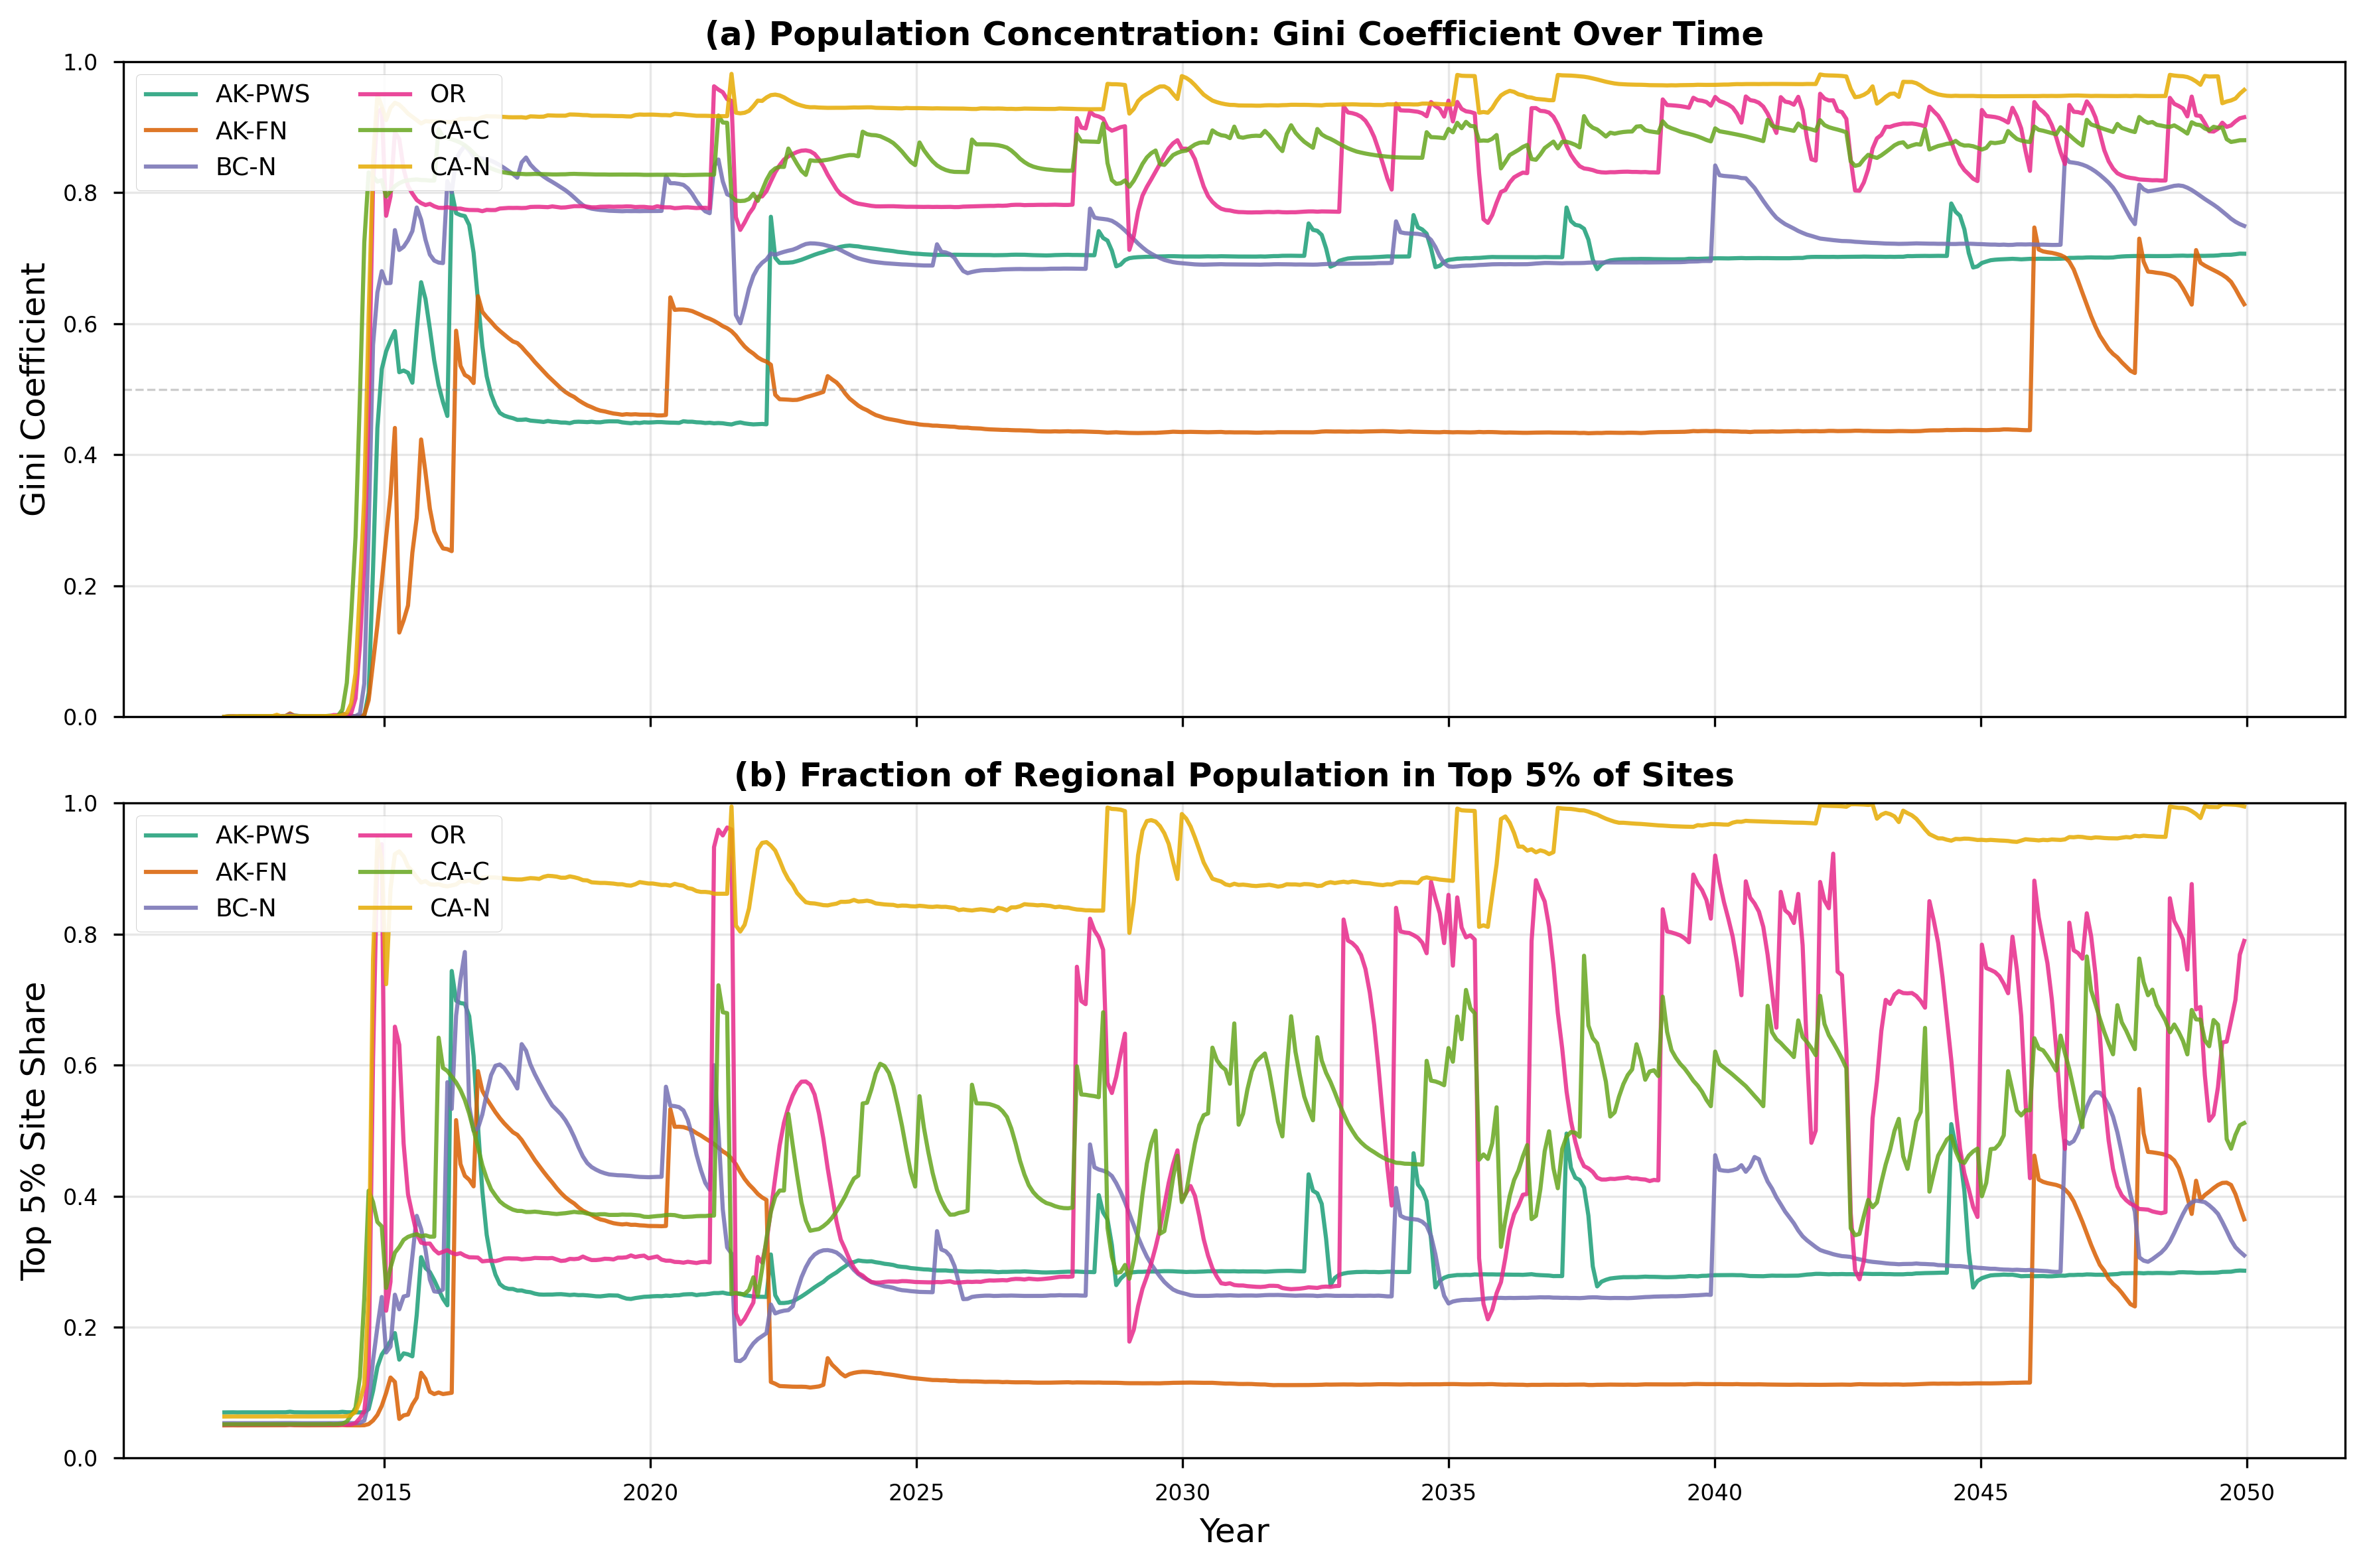
\includegraphics[width=0.80\textwidth]{figures/fig_oasis_concentration.png}
    \caption{Population concentration metrics over time for six key regions. \textbf{Left:} Gini coefficient of within-region site-level population distribution (0 = perfectly equal, 1 = all population in one site). Oregon (Gini $>$ 0.85 by 2050) shows extreme oasis concentration; AK-PWS and AK-FN (Gini $\approx$ 0.65) maintain distributed populations. \textbf{Right:} Fraction of regional population held by the top 3 sites over time. In Oregon, the top 3 sites hold 40--80\% of the population throughout the forecast period, while in Alaska they hold only 25--30\%.}
    \label{fig:oasis_concentration}
\end{figure}
    (Figure~\ref{fig:oasis_concentration})
\end{itemize}

\noindent
This concentration develops progressively over the simulation.  Pre-disease
(2012), population is uniformly distributed across all 59 sites at carrying
capacity ($K = 5{,}000$ each, Gini $= 0.00$).  By 2016, the post-crash population
is already uneven (Gini $\approx 0.78$), with only 38 sites retaining any
individuals.  By 2028, the oasis pattern is fully established: Gini exceeds
0.90, and the top 3 sites hold $\sim$80\% of the regional total
(Figure~\ref{fig:oasis_concentration}).

% --- Figure: Site Decomposition (oasis analysis) ---
\begin{figure}[!htbp]
    \centering
    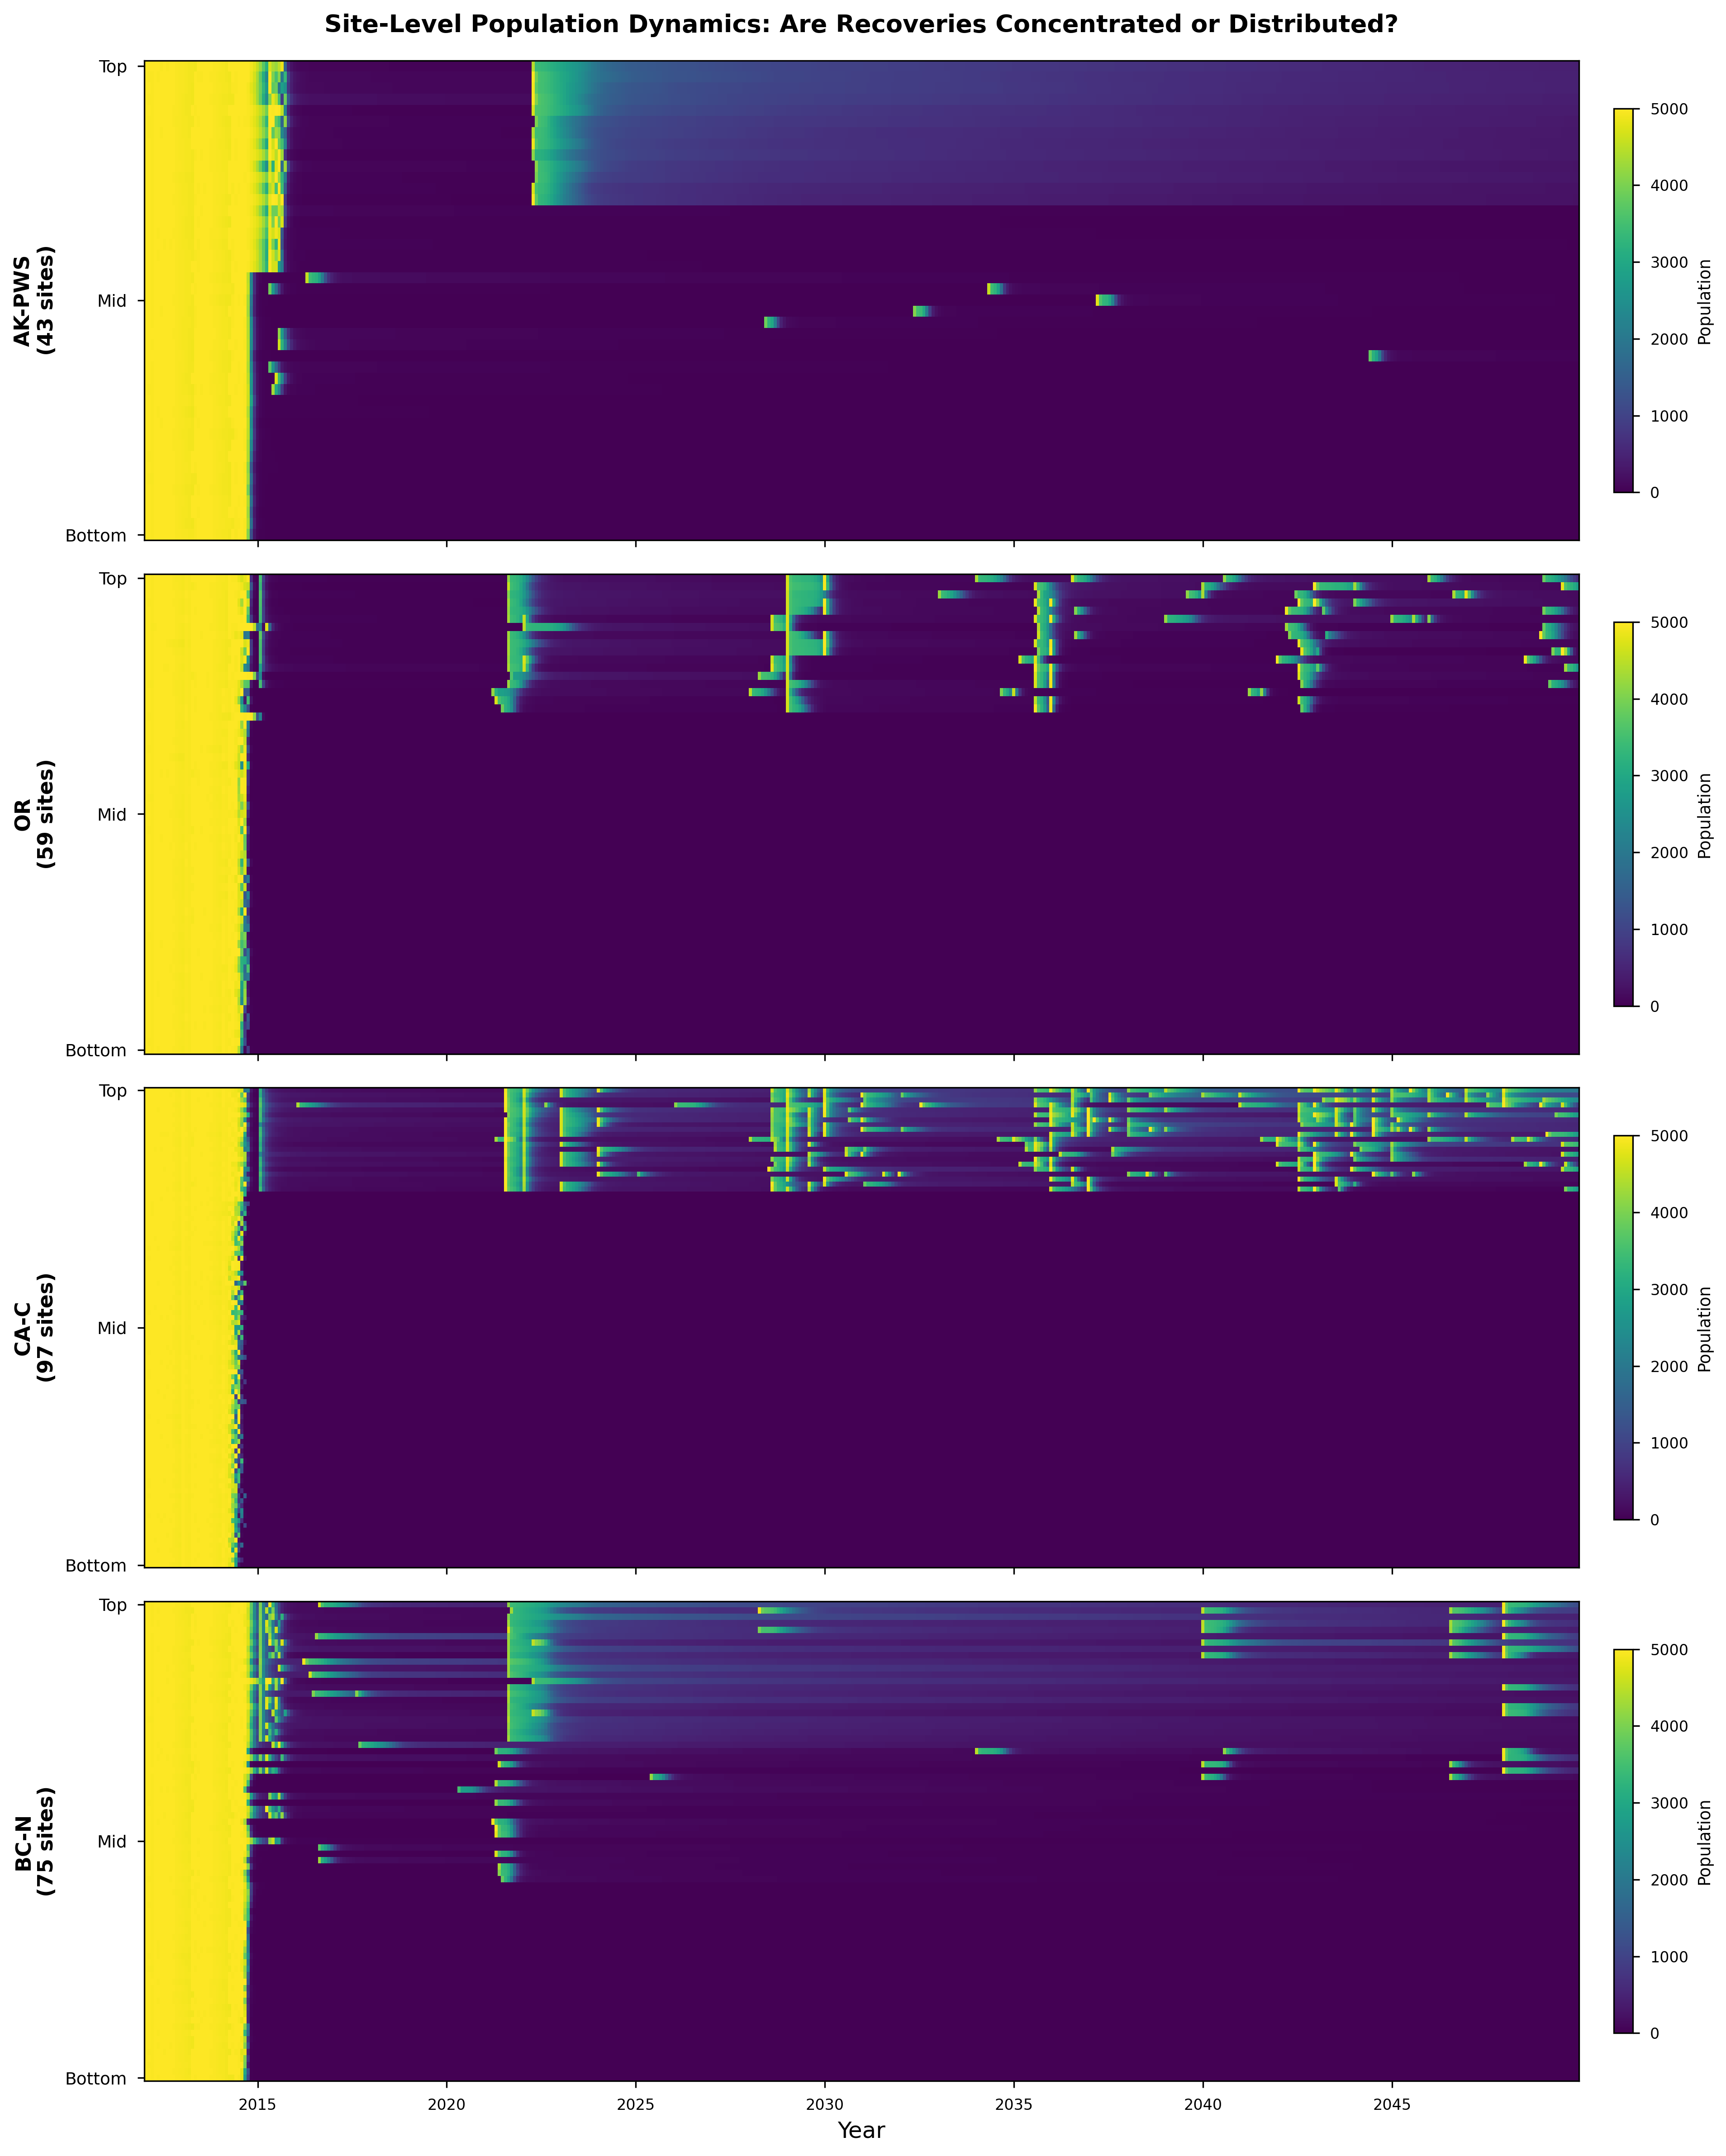
\includegraphics[width=0.85\textwidth]{figures/fig_site_decomposition.png}
    \caption{Site-level population dynamics within four key regions under the baseline scenario (F01, seed 42). Each panel shows the population trajectory of individual sites (thin lines) against the regional total (thick black line). In Oregon and CA-C, a handful of ``oasis'' sites hold the majority of the population, while in AK-PWS and AK-FN, population is broadly distributed across many sites. The boom-bust cycles visible at the regional level are driven by different subsets of sites in each cycle.}
    \label{fig:site_decomposition}
\end{figure>

% --- Figure: Oasis Concentration ---
\begin{figure}[!htbp]
    \centering
    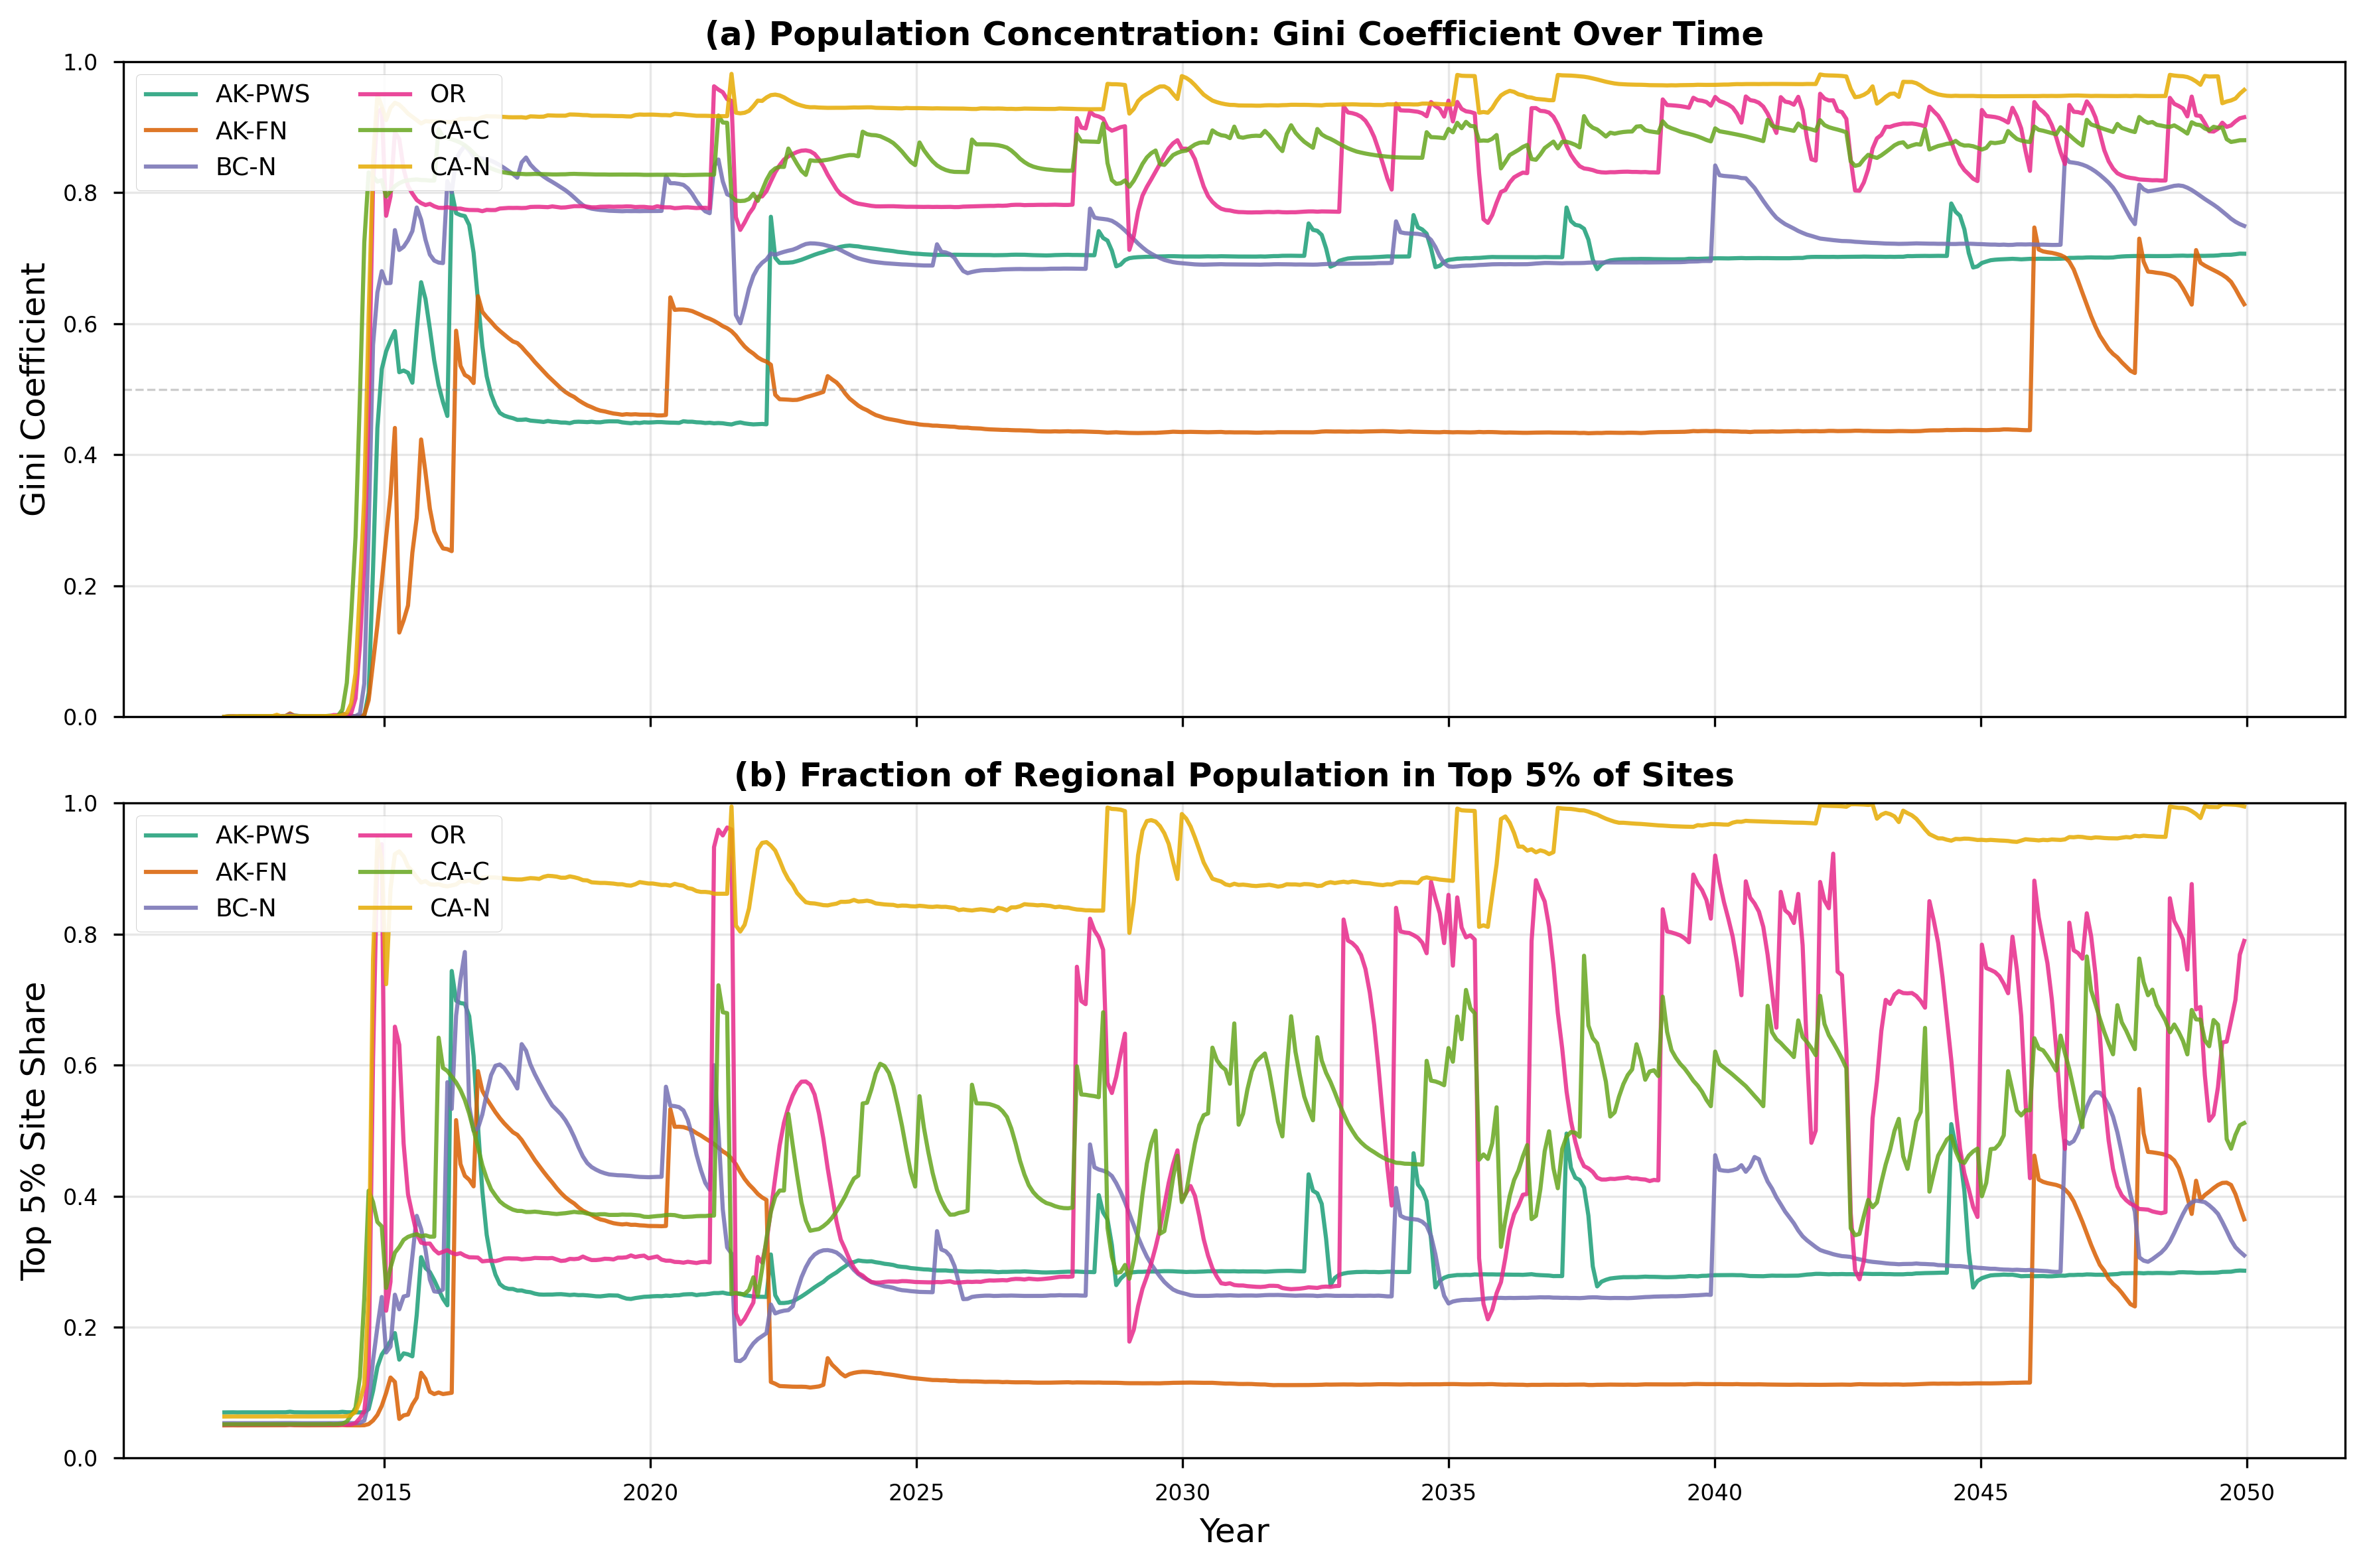
\includegraphics[width=0.80\textwidth]{figures/fig_oasis_concentration.png}
    \caption{Population concentration metrics over time for six key regions. \textbf{Left:} Gini coefficient of within-region site-level population distribution (0 = perfectly equal, 1 = all population in one site). Oregon (Gini $>$ 0.85 by 2050) shows extreme oasis concentration; AK-PWS and AK-FN (Gini $\approx$ 0.65) maintain distributed populations. \textbf{Right:} Fraction of regional population held by the top 3 sites over time. In Oregon, the top 3 sites hold 40--80\% of the population throughout the forecast period, while in Alaska they hold only 25--30\%.}
    \label{fig:oasis_concentration}
\end{figure>

The oasis sites are geographically clustered.  In all three seeds, the dominant
survivors concentrate along the southern Oregon coast between 42.0\textdegree N
and 42.8\textdegree N---a $\sim$90~km stretch from roughly Brookings to Gold
Beach.  This clustering suggests that the oasis phenomenon is not random but
reflects favorable local conditions at these latitudes, likely a combination
of cooler upwelling-influenced SSTs and strong tidal flushing that suppresses
the environmental pathogen pool.

\subsubsection{Oasis Identity Is Stochastic, Oasis Geography Is Not}

A striking finding emerges from cross-seed comparison: while the oasis
\textit{zone} is consistent (southern Oregon, $\sim$42--43\textdegree N), the
specific sites that dominate vary substantially across random seeds.  Across
three seeds, 13 different sites appear among the top 5 in at least one seed,
but only 2 sites appear in the top 5 in more than one seed.  In seed 42,
OR-048 (42.67\textdegree N) holds 37\% of the regional population; in seed 999,
OR-020 (44.60\textdegree N)---a site 220~km to the north---is the dominant oasis.

This stochasticity has a clear mechanistic origin.  At the small population
sizes that characterize post-crash Oregon ($\sim$400--2{,}000 individuals spread
across the region), sweepstakes reproductive success \citep{hedgecock2011}
and Allee effects create enormous variance in which sites happen to produce
successful recruitment events.  A site that, by chance, produces a successful
larval cohort in one year can temporarily dominate the regional population
through exponential growth from a low base.  The same site in a different
random seed may fail to produce that initial cohort and remain near zero.

% --- Figure: Oasis Consistency ---
\begin{figure}[!htbp]
    \centering
    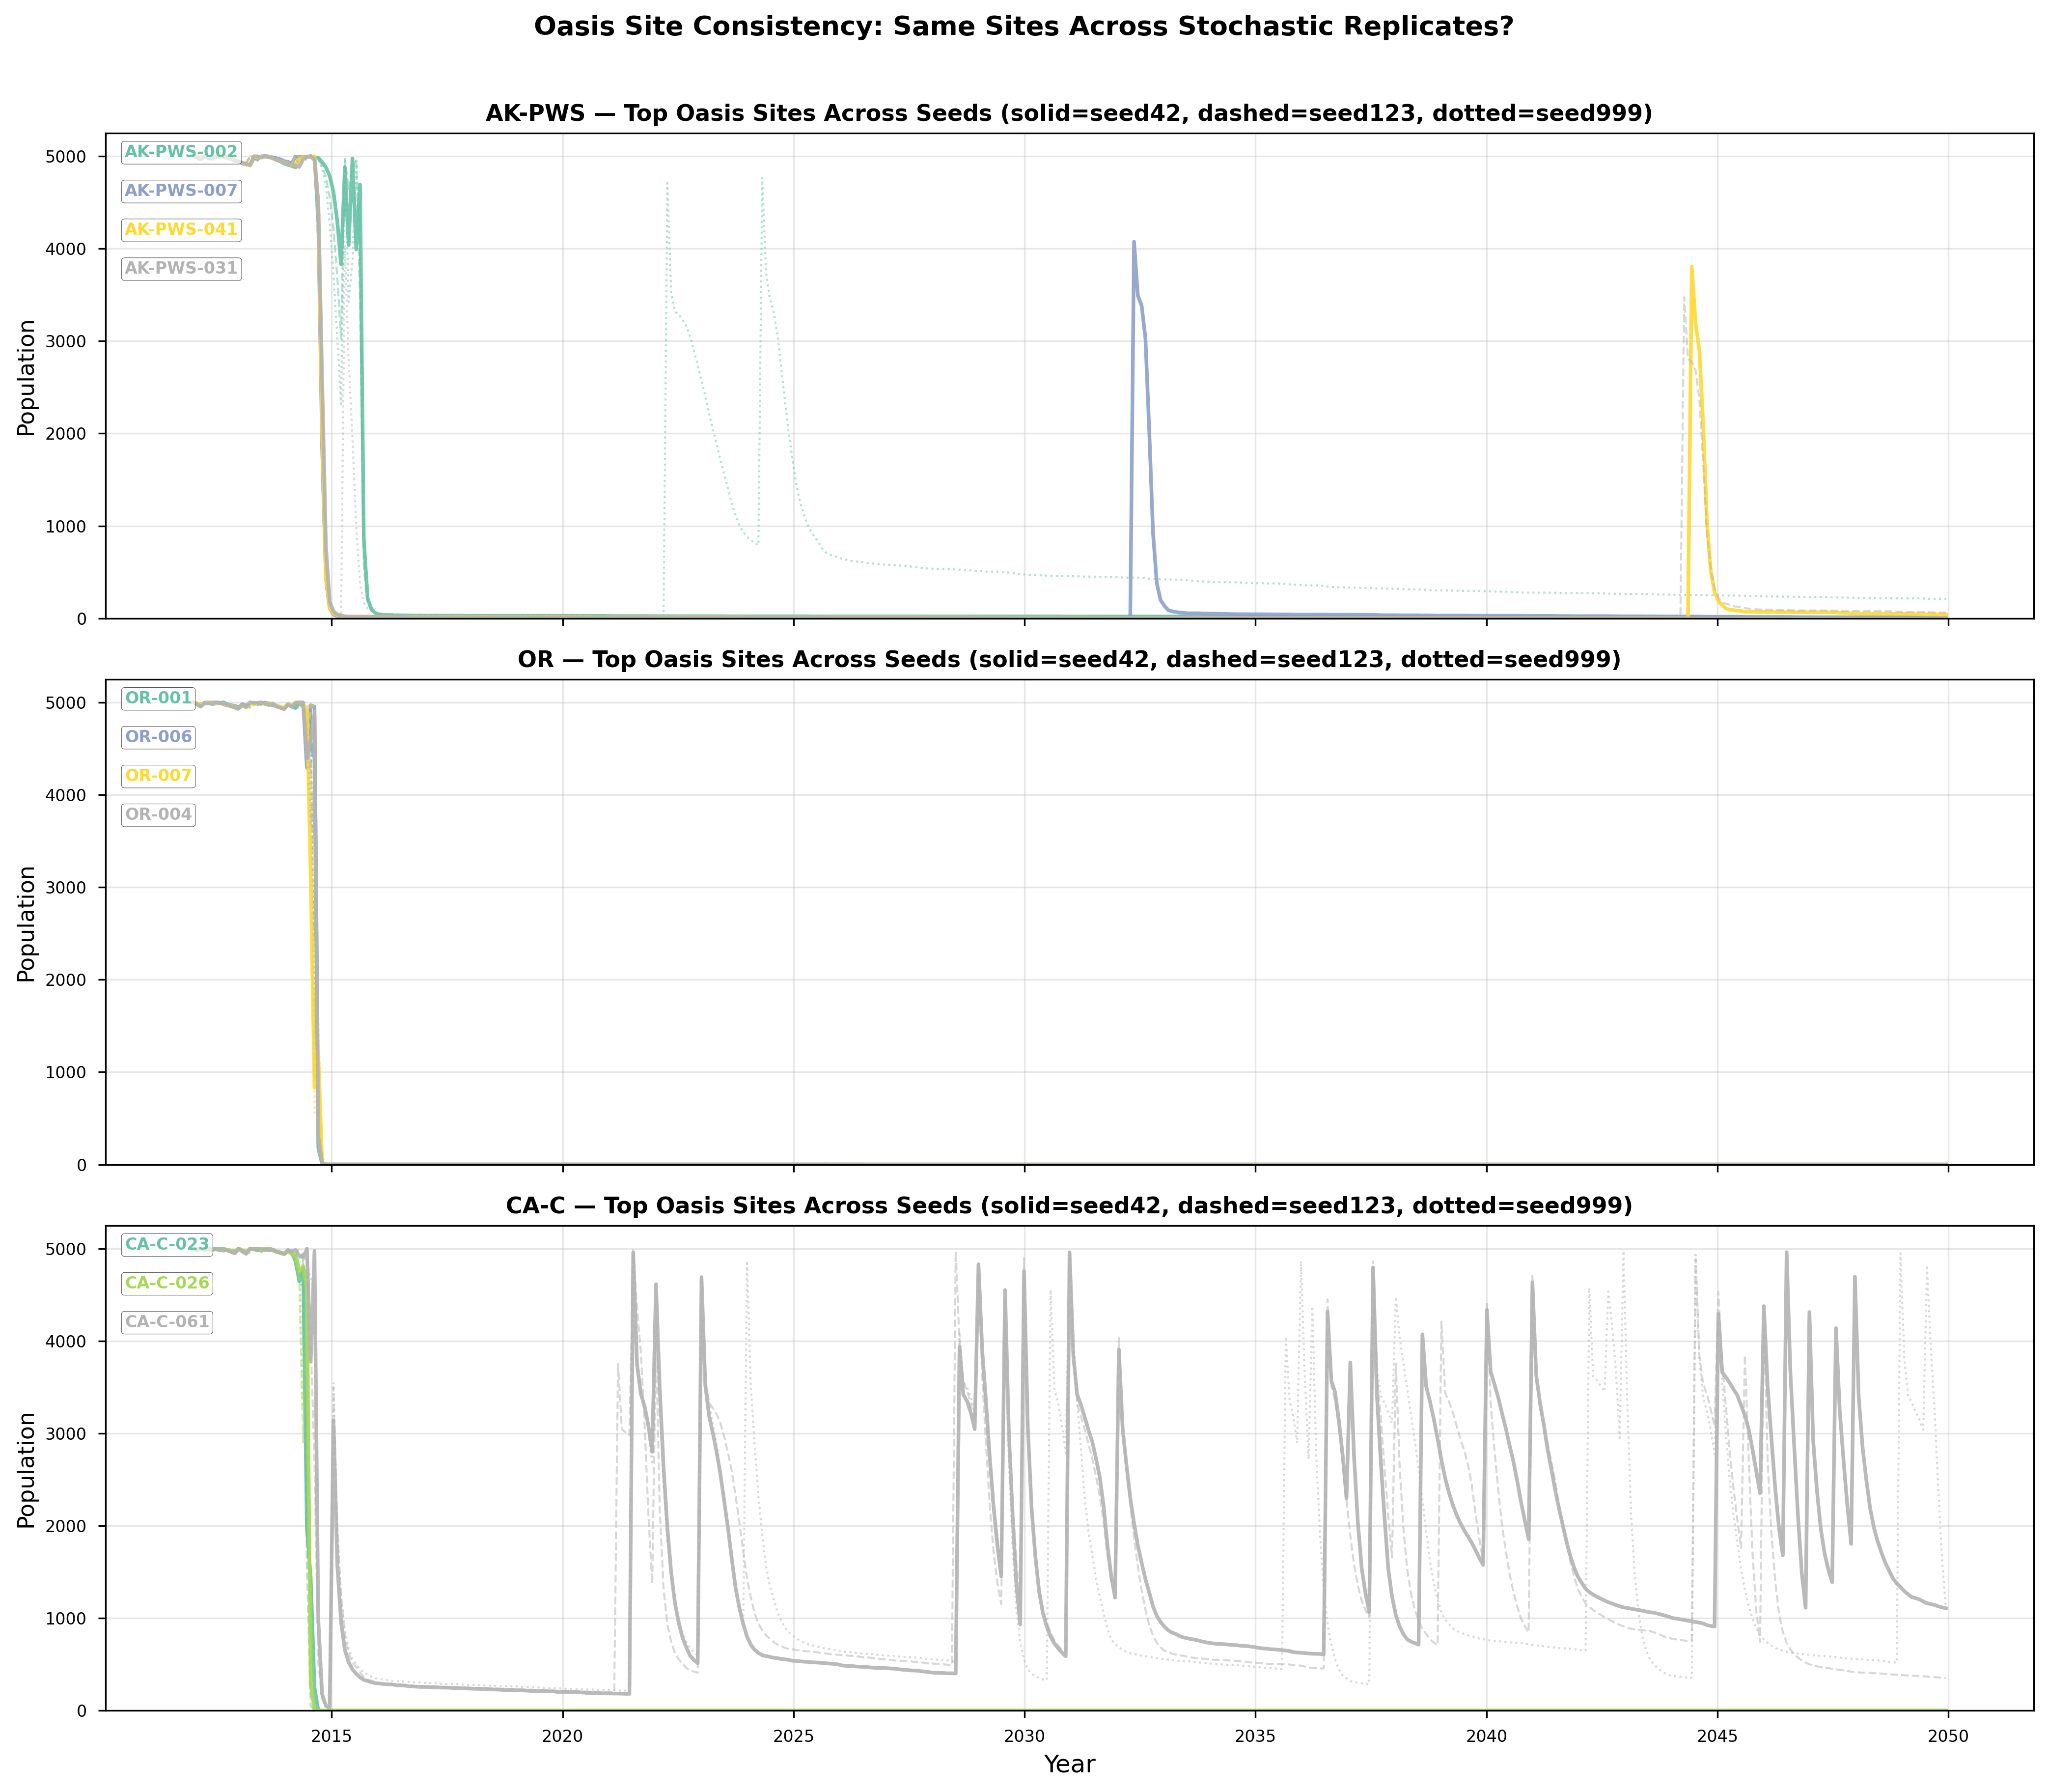
\includegraphics[width=0.90\textwidth]{figures/fig_oasis_consistency.png}
    \caption{Cross-seed consistency of oasis site identity in Oregon. Population trajectories of the top 5 Oregon sites under each of three independent random seeds. While the geographic \textit{zone} of oasis concentration is consistent (southern Oregon, 42--43\textdegree N), the specific sites that dominate vary across seeds: 13 different sites appear among the top 5 across three seeds, with only 2 appearing in more than one seed. Oasis geography is deterministic but oasis identity is stochastic, reflecting the role of sweepstakes reproductive success at small population sizes.}
    \label{fig:oasis_consistency}
\end{figure>

The conservation implication is important: \textbf{oasis sites cannot be
identified in advance from geographic or oceanographic data alone.}  While the
southern Oregon coast is consistently favorable, the specific sites that
sustain the population depend on stochastic reproductive events that are
inherently unpredictable.  Monitoring programs should therefore survey the
entire favorable zone rather than focusing on a few ``expected'' oasis sites.

% --- Figure: Oasis Consistency ---
\begin{figure}[!htbp]
    \centering
    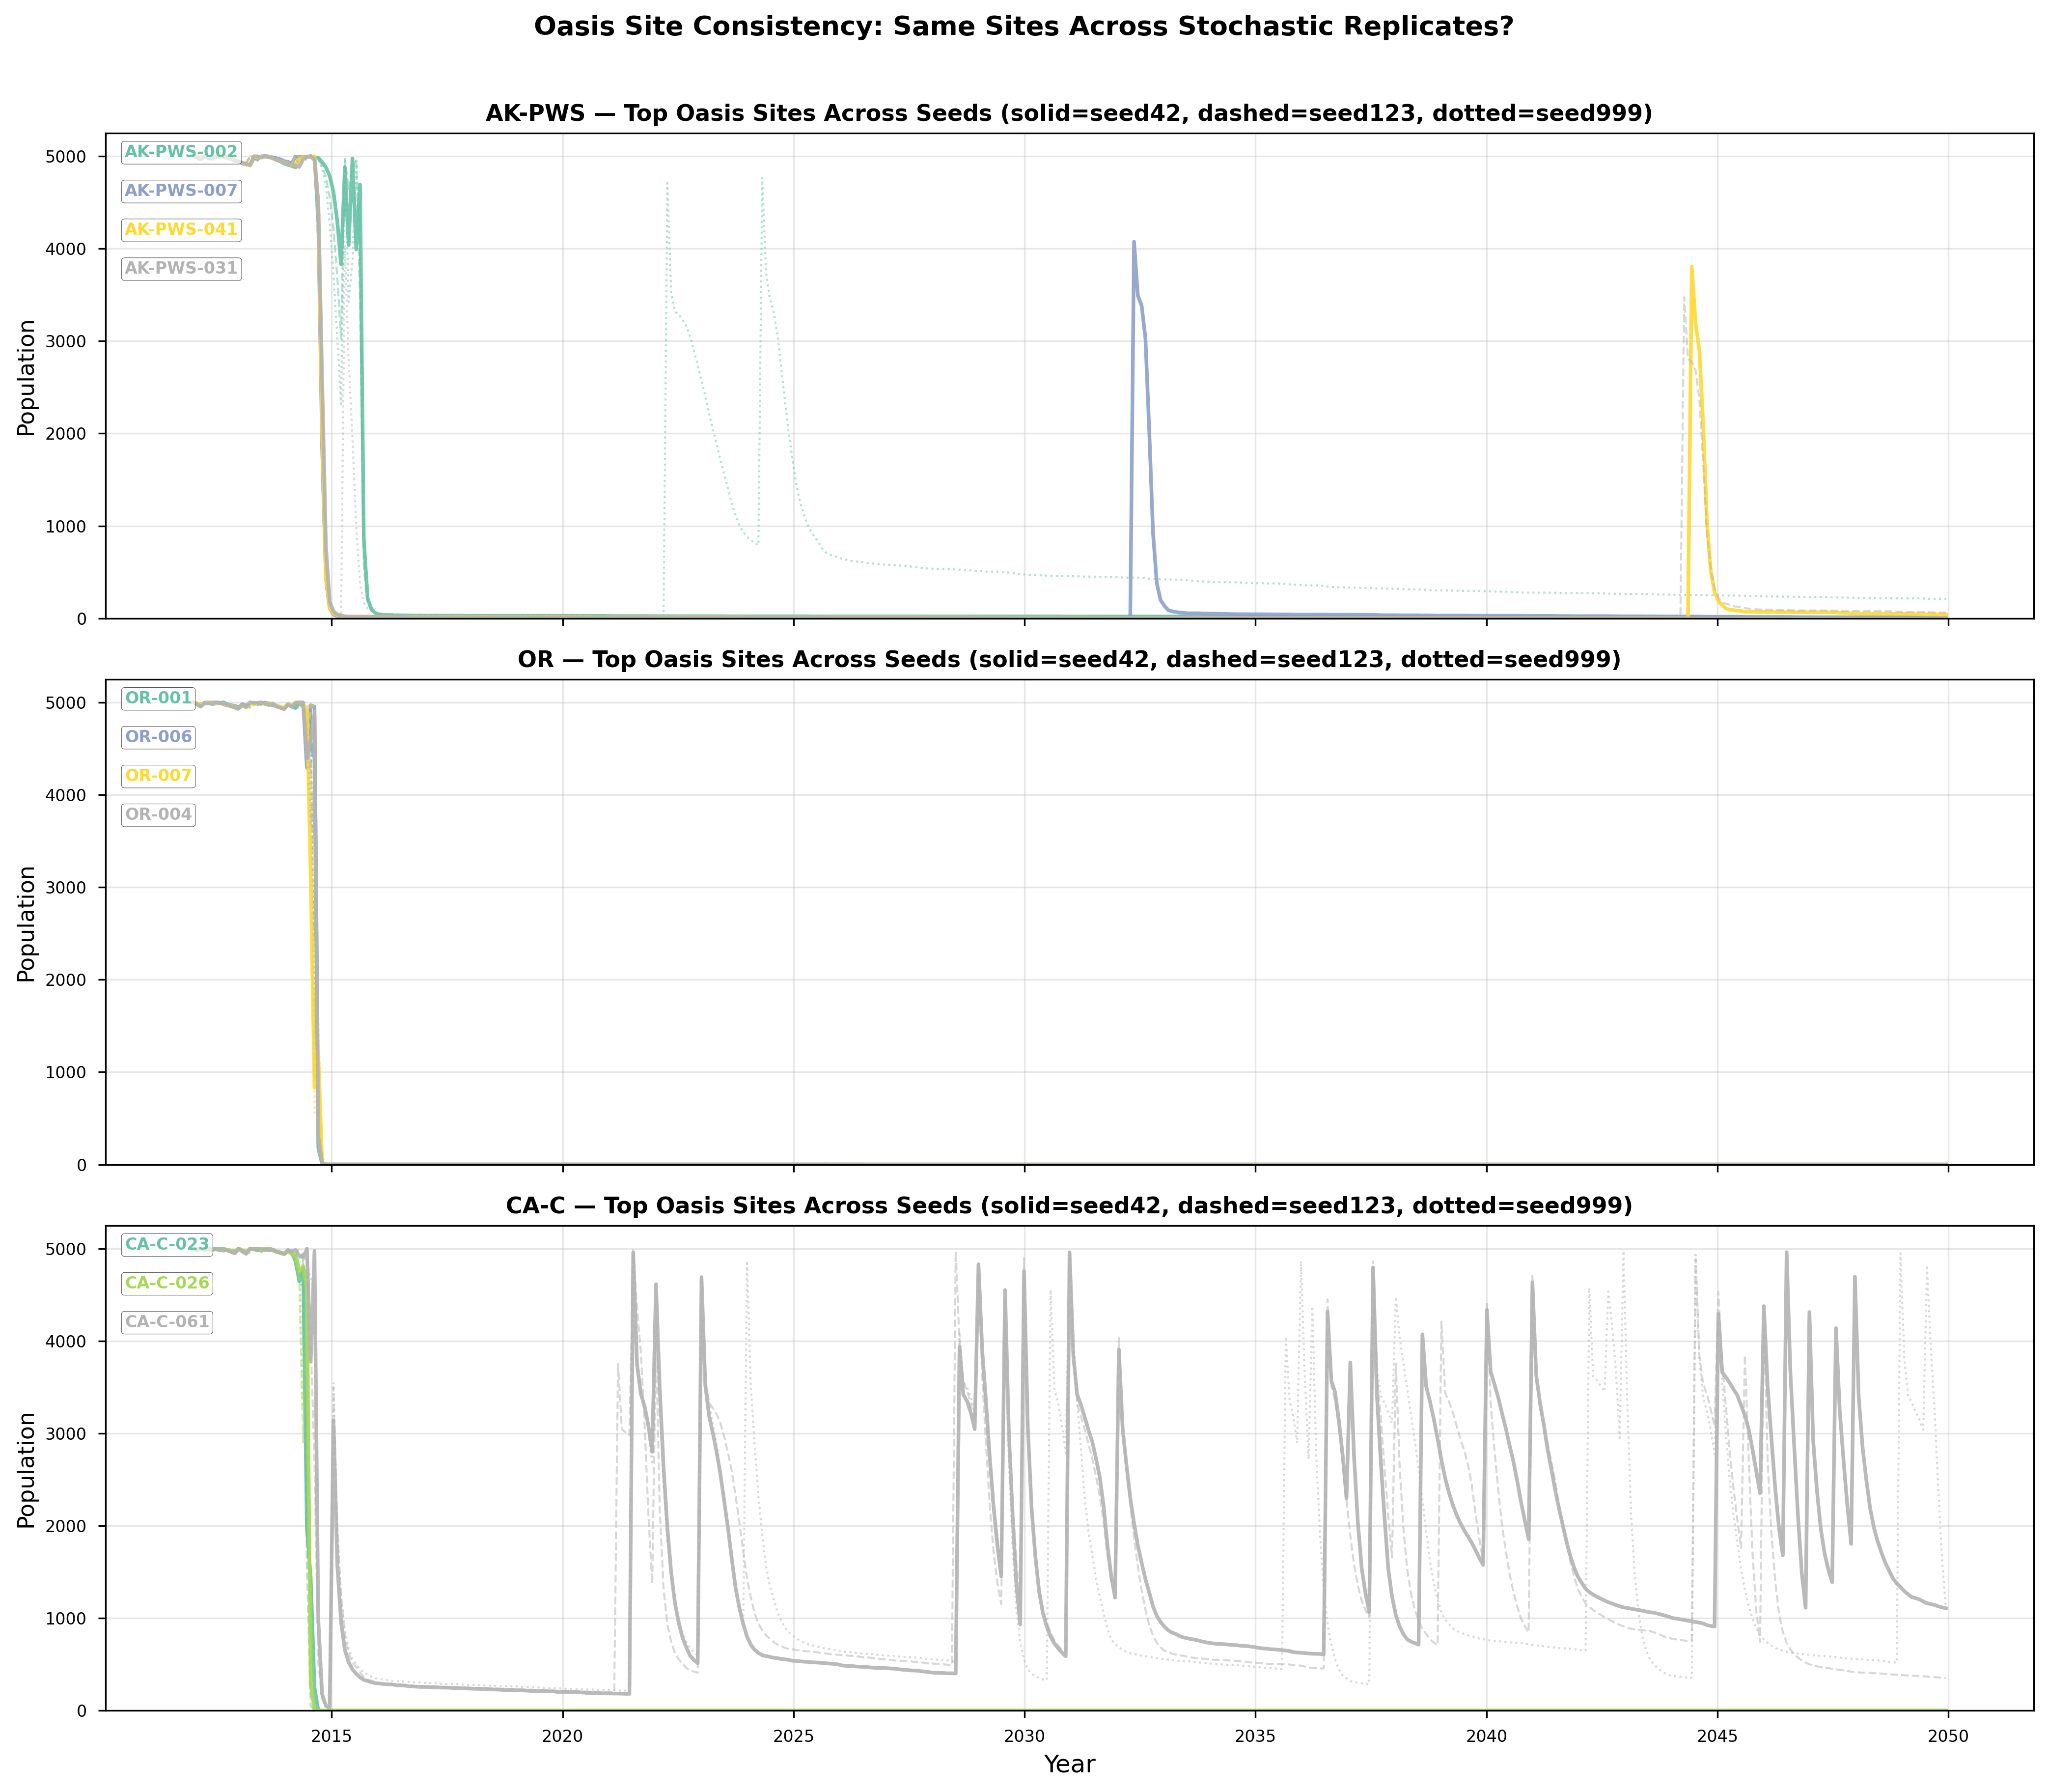
\includegraphics[width=0.90\textwidth]{figures/fig_oasis_consistency.png}
    \caption{Cross-seed consistency of oasis site identity in Oregon. Population trajectories of the top 5 Oregon sites under each of three independent random seeds. While the geographic \textit{zone} of oasis concentration is consistent (southern Oregon, 42--43\textdegree N), the specific sites that dominate vary across seeds: 13 different sites appear among the top 5 across three seeds, with only 2 appearing in more than one seed. Oasis geography is deterministic but oasis identity is stochastic, reflecting the role of sweepstakes reproductive success at small population sizes.}
    \label{fig:oasis_consistency}
\end{figure}

\subsubsection{Distributed Recovery in Alaska}

The Alaskan pattern is strikingly different.  In Prince William Sound (AK-PWS),
recovery is broad-based:

\begin{itemize}
  \item 37--38 of 43 sites retain population by 2050 (86--88\% of sites)
  \item The top 3 sites hold only 25--29\% of the regional population
  \item Gini coefficients remain moderate at 0.65--0.71
\end{itemize}

\noindent
Similarly, Fairweather North (AK-FN) maintains population across 37--40 of 40
sites (93--100\%), with Gini values of 0.63--0.66.  Alaska's distributed
persistence reflects two features of its thermal regime: (1) cold winter
temperatures suppress the pathogen broadly across all sites, not just at
favorable microhabitats; and (2) larval connectivity among nearby sites is
high, so recruitment events replenish depleted sites from the regional pool
rather than concentrating at a single source.

This contrast has practical implications for population monitoring.  In Alaska,
a random transect across the region will provide a representative estimate of
overall abundance.  In Oregon, a random transect will likely miss the oasis
sites entirely, producing an underestimate that could differ from the true
regional population by an order of magnitude.

\subsubsection{The Boom-Bust Cycle at Site Resolution}

The recruitment pulses described in Section~\ref{sec:trajectories} become
more dramatic when viewed at site resolution
(Figure~\ref{fig:site_decomposition}).  Oregon experiences repeated
boom-bust cycles (approximately every 3--4 years in the forecast period), and
each cycle is driven by a different combination of sites.  A typical boom
unfolds as follows:

\begin{enumerate}
  \item \textbf{Initiation (winter):} One or a few sites with surviving adults
    produce a successful larval cohort during the winter spawning season, when
    pathogen activity is suppressed by cold temperatures.
  \item \textbf{Amplification (spring):} Recruits grow rapidly and begin to
    reproduce themselves.  If multiple neighboring sites receive larvae from
    the same source (or from each other), the boom propagates along the coast.
  \item \textbf{Peak (late spring/early summer):} The regional population
    surges, sometimes by an order of magnitude within 6 months.  At peak,
    even a few thousand individuals across the region represent a dramatic
    improvement from the inter-boom nadir of a few hundred.
  \item \textbf{Crash (summer):} Rising SSTs reactivate the pathogen.
    The temporarily elevated host density amplifies the environmental pathogen
    pool through the shedding--infection positive feedback, and disease sweeps
    through the boom cohort.  Within 3--6 months, the regional population
    returns to near its pre-boom level.
\end{enumerate}

Importantly, the sites that initiate each boom are not always the same sites
that initiated the previous boom.  The stochastic nature of sweepstakes
reproduction, combined with the tiny population sizes between booms, means
that oasis identity shuffles between cycles.  However, the \textit{geographic
zone} from which booms originate remains consistent: the southern Oregon
coast, where the thermal regime most strongly favors winter recovery.

% --- Figure: Boom Decomposition ---
\begin{figure}[!htbp]
    \centering
    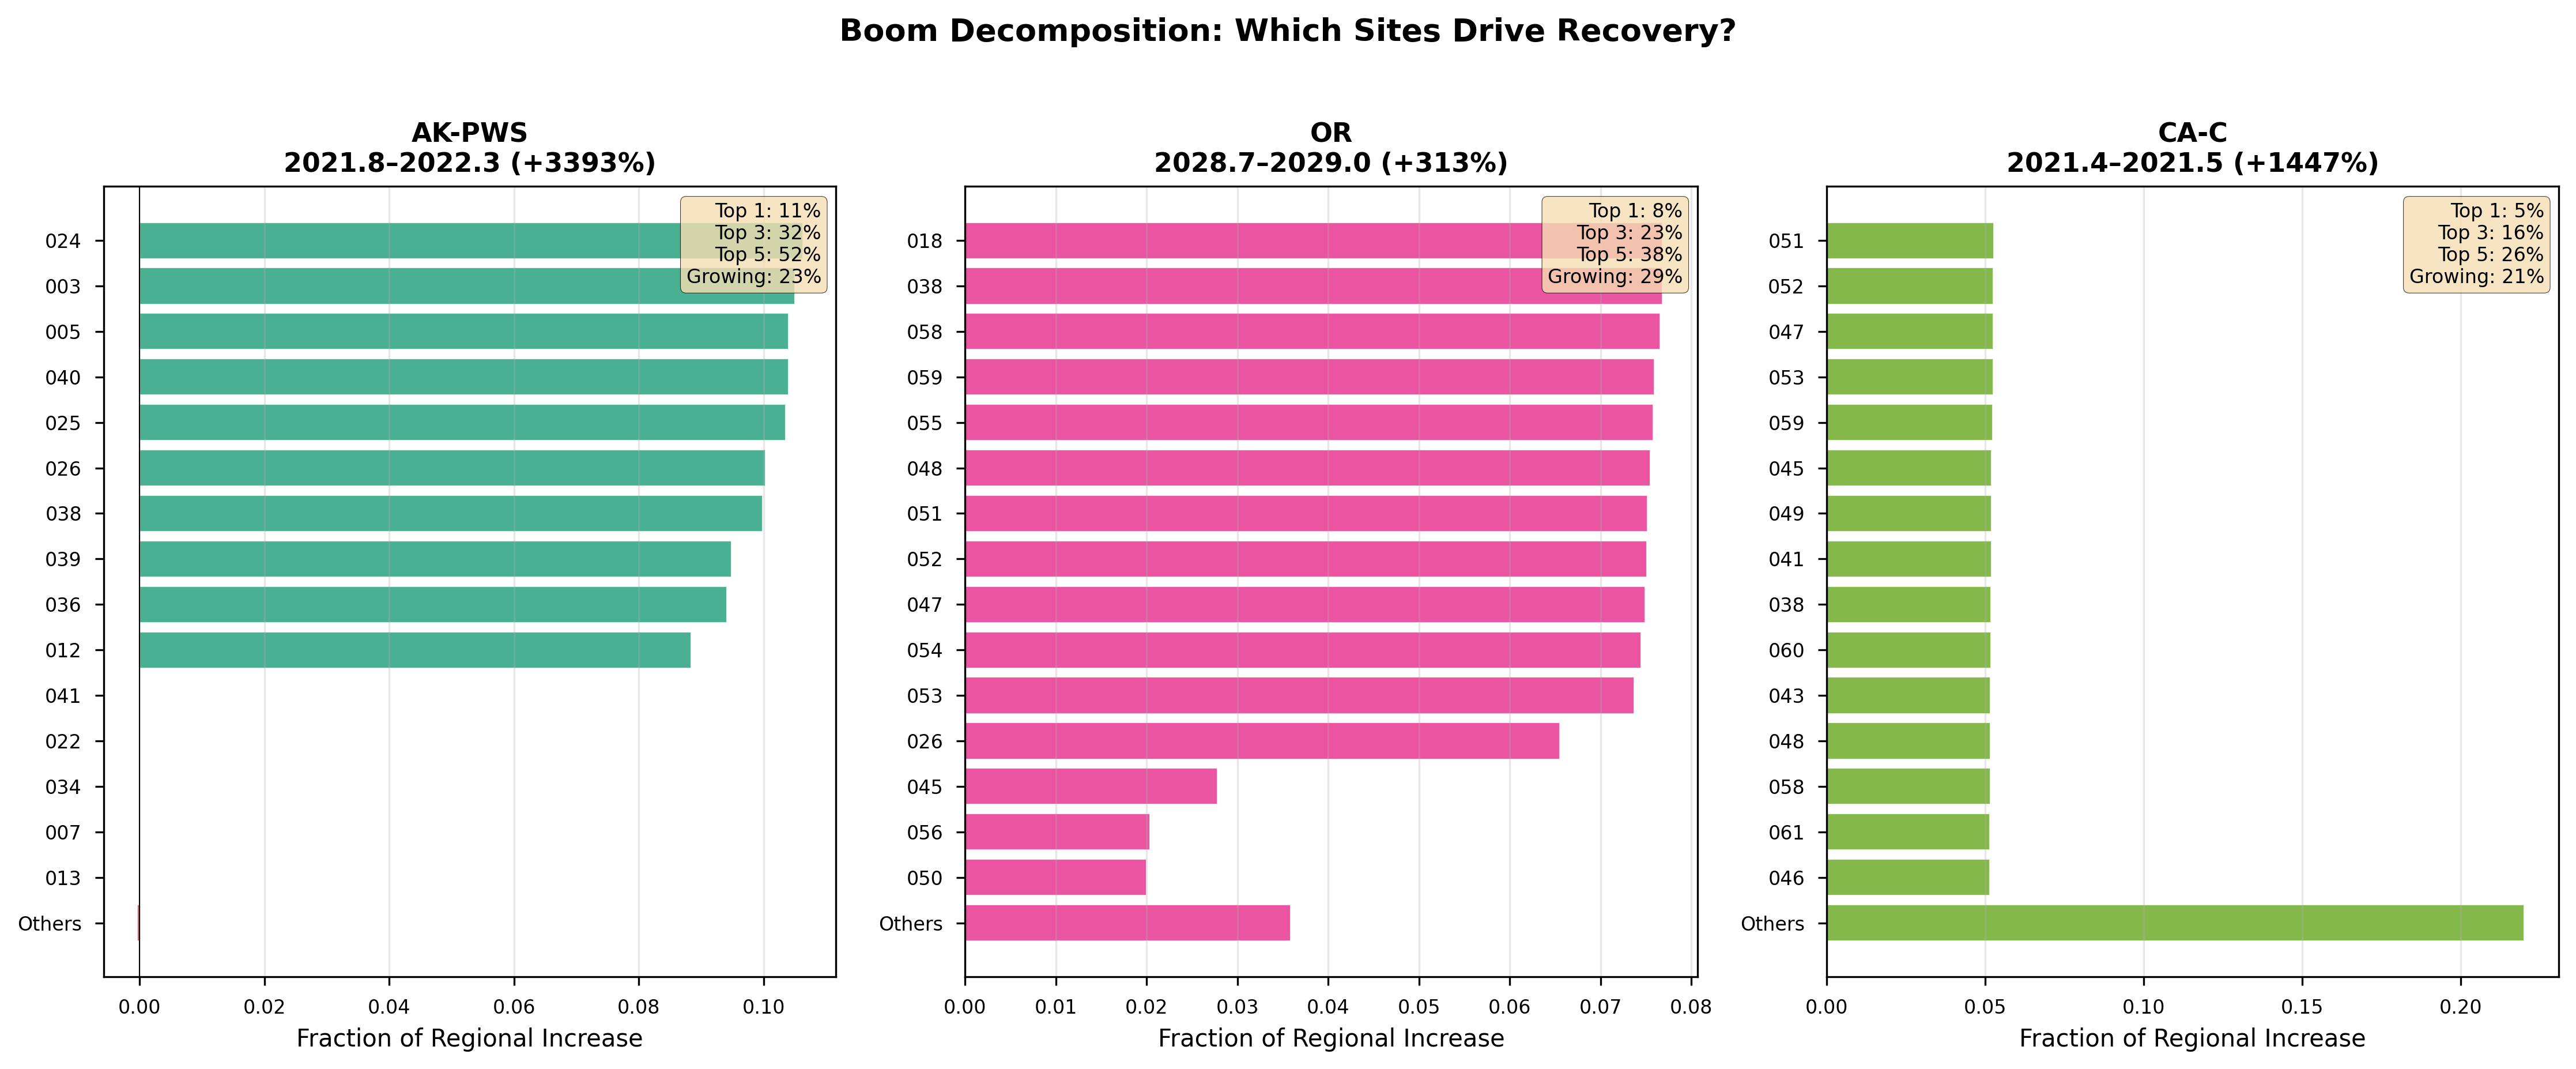
\includegraphics[width=0.85\textwidth]{figures/fig_boom_decomposition.png}
    \caption{Decomposition of selected recovery booms into individual site contributions. For each boom event (identified as periods where regional population increases by $>$50\% within 6 months), bars show each site's absolute contribution to the regional population increase, ranked from largest to smallest. In Oregon, a single site often contributes $>$40\% of the boom; in AK-PWS, the largest contributor accounts for only $\sim$10\%. This confirms the oasis-driven nature of Oregon recovery versus the distributed recovery in Alaska.}
    \label{fig:boom_decomposition}
\end{figure}

\subsubsection{Implications for Conservation}

The oasis analysis yields three actionable findings:

\begin{enumerate}
  \item \textbf{Oregon's ``recovery'' is fragile.}  A regional recovery
    rate of 17.6\% sounds encouraging, but when this population is
    concentrated in 2--3 sites with $\sim$80\% of the total, it is
    vulnerable to a single localized catastrophe (an oil spill, a hypoxia
    event, a point-source pollutant) that could eliminate the majority
    of the regional population in a single event.

  \item \textbf{Reintroduction should target oasis zones, not specific
    sites.}  Because oasis identity is stochastic but oasis geography is
    consistent, captive breeding releases should distribute individuals
    across the favorable zone (e.g., multiple sites along the southern
    Oregon coast) rather than concentrating them at a single site that
    may or may not become a successful oasis.

  \item \textbf{Northern populations are more resilient to local
    disturbance.}  The distributed persistence pattern in Alaska means
    that losing any single site has a small impact on regional population
    viability.  This inherent redundancy makes Alaskan populations better
    candidates for long-term self-sustaining recovery, even though their
    absolute numbers are currently lower than Oregon's.
\end{enumerate}


% ============================================================
% SECTION 5: Model Description
% ============================================================
% ==============================================================================
% Section 5: Model Description
% ==============================================================================

\section{Model Description}
\label{sec:model}

This section describes the structure and mechanics of the SSWD-EvoEpi
agent-based model.  Readers interested primarily in conservation
implications may proceed to the Discussion (Section~\ref{sec:discussion});
what follows is intended for those who wish to understand how the
forecasts were generated.

% --------------------------------------------------------------------------
\subsection{Agent-Based Framework}
\label{sec:abm_framework}

The model simulates individual \textit{Pycnopodia helianthoides} across
\textbf{896 coastal sites} spanning the species' entire historical range,
from the western Aleutian Islands (52.5\textdegree N) to central Baja
California (28.5\textdegree N).  Sites are grouped into 18 geographic
regions corresponding to major oceanographic and biogeographic boundaries
(e.g., Prince William Sound, Salish Sea, Oregon coast, Channel Islands).
Each site supports up to $K = 5{,}000$ individuals, yielding a theoretical
coast-wide carrying capacity of approximately 4.5~million sea stars.

% --- Figure: Network Map (from progress report) ---
\begin{figure}[!htbp]
    \centering
    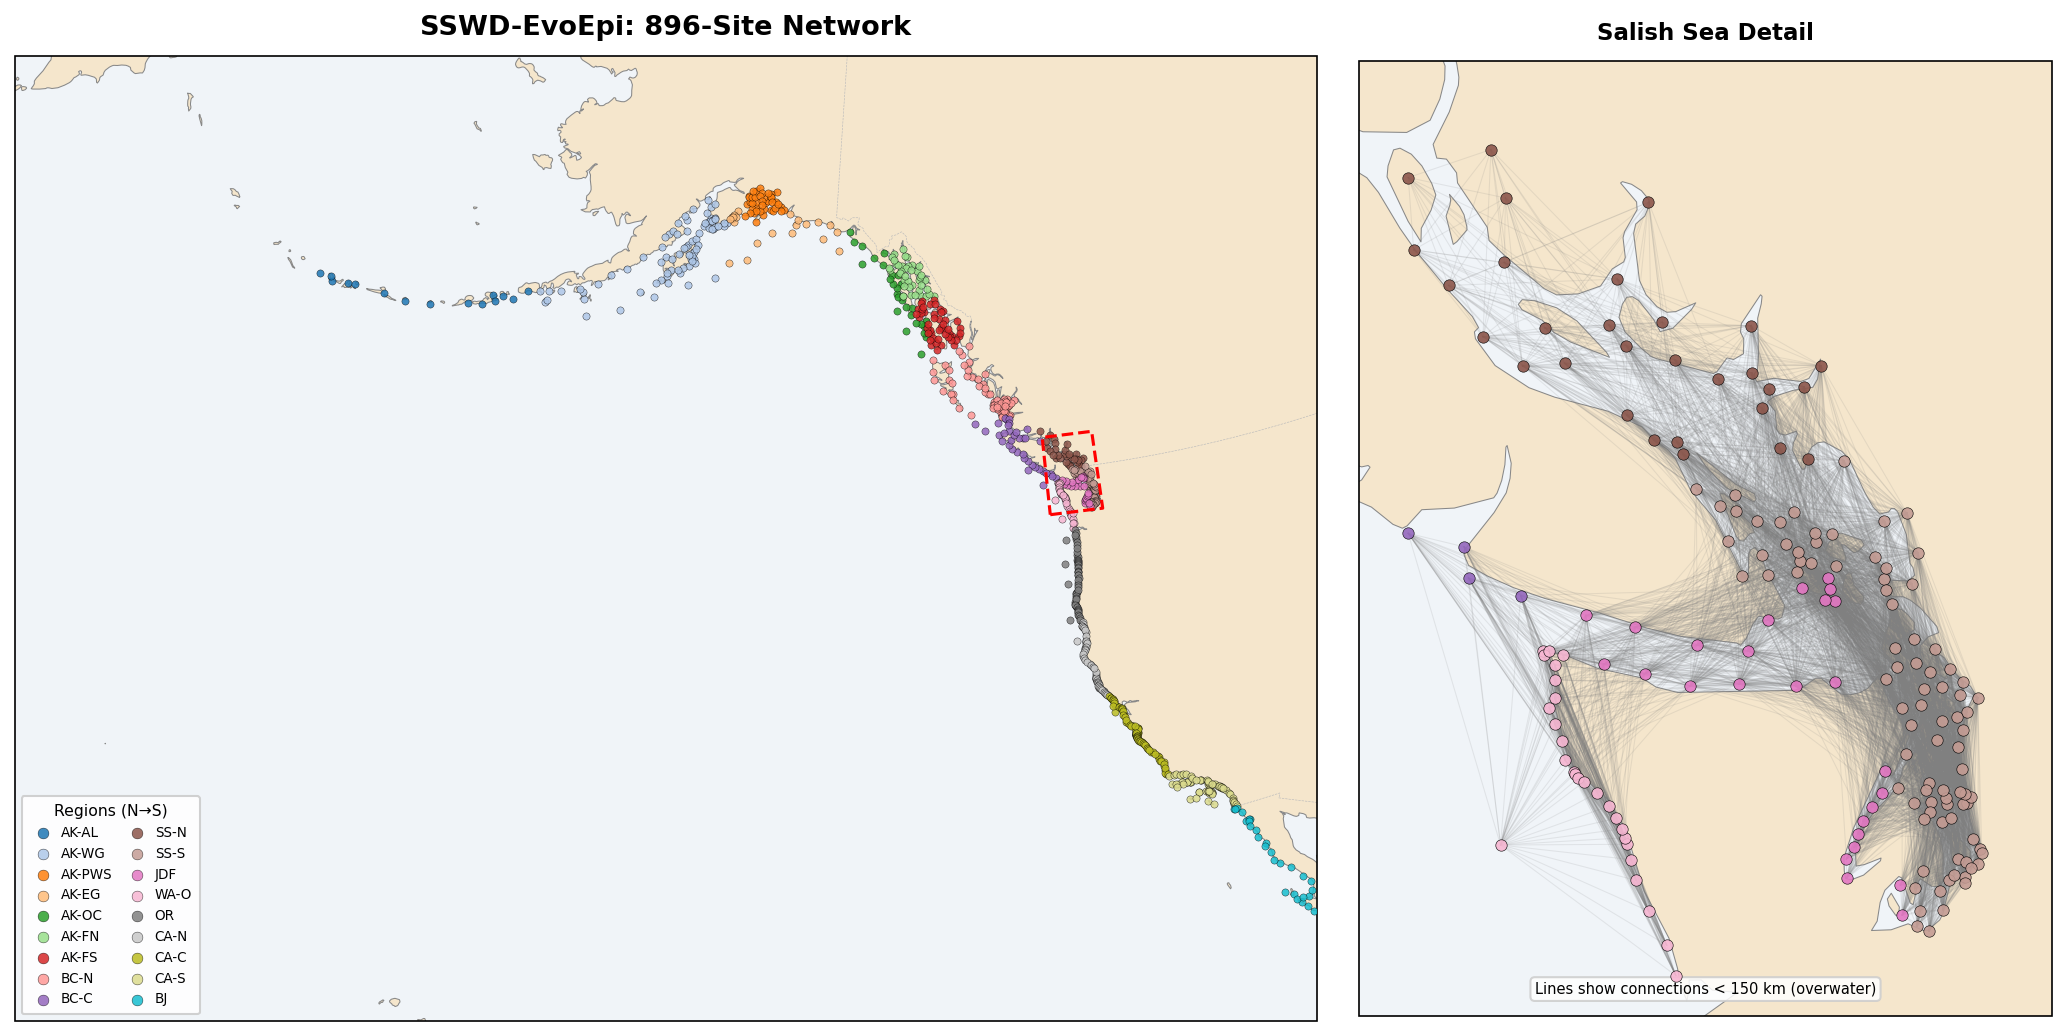
\includegraphics[width=0.85\textwidth]{figures/fig_network_map.png}
    \caption{The 896-site spatial network spanning Alaska (Aleutian Islands) to Baja California, colored by 18 geographic regions. Sites are connected by larval dispersal ($D_L = 400$~km exponential decay) and waterborne pathogen transport ($D_P = 300$~km) kernels. The inset panel zooms into the Salish Sea, where gray connectivity lines illustrate the dense local network structure through which larvae and pathogen disperse.}
    \label{fig:network_map}
\end{figure}

The simulation operates in \textbf{daily timesteps} from 2012 through 2050.
Each simulated day steps through disease transmission, individual survival,
growth, and---during the spawning season---reproduction and larval dispersal.

Each individual sea star is represented as a distinct agent carrying the
following attributes:
\begin{itemize}
  \item \textbf{Position} ($x, y$ in meters) and \textbf{heading}
        (direction of travel) within its home site;
  \item \textbf{Body size} (arm-tip diameter in mm, growing via von
        Bertalanffy dynamics toward $L_\infty = 1{,}000$\,mm);
  \item \textbf{Age} and \textbf{sex};
  \item \textbf{Disease state} (susceptible, exposed, pre-symptomatic,
        symptomatic, or dead);
  \item \textbf{51 genetic loci} governing three heritable defense traits
        (Section~\ref{sec:host_genetics}).
\end{itemize}

Individuals move within sites via a \textbf{correlated random walk} at a
base speed of 0.5\,m/min \citep{hodin2021}, resolved in 24 hourly substeps
per day.  Symptomatic individuals slow to 10\% of normal speed; dead
individuals do not move.  Movement matters because disease transmission is
\textbf{spatially explicit}: a 20\,m grid within each site tracks local
pathogen concentrations, so stars near clusters of infected individuals
experience higher exposure than those farther away.

\paragraph{Temperature forcing.}
All scenarios are driven by \textbf{observed sea surface temperature (SST)}
from the NOAA Optimum Interpolation SST v2.1 dataset for 2012--2025,
bilinearly interpolated to each of the 896 model sites.  For the projection
window (2026--2050), SSTs are generated via a delta method applied to CMIP6
general circulation models (Section~\ref{sec:sst_projections}).  Real
climate events---including the 2013--2016 marine heatwave, El~Ni\~no, and
La~Ni\~na cycles---are thus automatically incorporated during the
historical period.

% --------------------------------------------------------------------------
\subsection{Disease Mechanics}
\label{sec:disease}

The disease module simulates the dynamics of \textit{Vibrio pectenicida},
recently confirmed as the etiological agent of SSWD through fulfillment of
Koch's postulates \citep{prentice2025}.  Its structure rests on two
biological pillars: a modified SEIR compartmental model within individual
hosts, and the VBNC (viable but non-culturable) dormancy state that couples
pathogen activity to water temperature.

\paragraph{Within-host progression.}
Each individual follows a five-stage disease progression:
\begin{center}
S $\to$ E $\to$ I$_1$ (pre-symptomatic) $\to$ I$_2$ (symptomatic)
  $\to$ Dead
\end{center}
Transition rates between compartments are Arrhenius-scaled (i.e., exponentially increasing with temperature) to local SST,
meaning disease progresses faster in warmer water.  At a reference
temperature of 20\textdegree C, the mean time from exposure to death is
approximately 6~days ($\mu_{EI_1} = 0.233$/d, $\mu_{I_1 I_2} = 0.434$/d,
$\mu_{I_2 D} = 0.563$/d).  Pre-symptomatic individuals shed pathogen at a
rate of $\sigma_1 = 5.0$ units/day; symptomatic individuals shed ten-fold
more ($\sigma_2 = 50.0$).  Dying stars release a burst of $\sigma_D = 15.0$
units.  Recovered individuals return to susceptible status---echinoderms
lack adaptive immunity, so reinfection is possible \citep{prentice2025}.

\paragraph{The VBNC state.}
\textit{Vibrio} species enter a dormant VBNC state in cold water
\citep{liu2019}.  We model this as a sigmoid transition centered at
$T_\mathrm{vbnc} = 12$\textdegree C (steepness $k = 2.0$): at
14\textdegree C the pathogen is ${\sim}$98\% active, at 12\textdegree C
it is 50\% active, and at 10\textdegree C only ${\sim}$2\% remains active.
A biophysical floor of $T_\mathrm{vbnc,min} = 9$\textdegree C prevents any
evolutionary adaptation below this temperature (Section~\ref{sec:pathogen_evo}).

This mechanism has profound geographic consequences.  In southern California,
where SST routinely exceeds 12\textdegree C, the pathogen is active
year-round and disease pressure is relentless.  In Alaska, where SST only
briefly exceeds the threshold in summer, stars receive a seasonal reprieve
during the cold months---but the pathogen persists in dormancy, ready to
reactivate each warm season.

\paragraph{Environmental pathogen pool.}
Each site maintains a dynamic environmental reservoir of \textit{Vibrio}.
The pool grows as infected individuals shed pathogen (fraction
$\alpha_\mathrm{env} = 0.18$ enters the persistent pool) and decays
naturally ($\delta_\mathrm{env} = 0.02$/day, half-life $\approx$35~days).
A susceptible star's daily infection probability follows Michaelis--Menten
kinetics with a half-saturation constant $K_\mathrm{half} = 800{,}000$,
modified by the individual's resistance trait, body size, and local VBNC
activation.  This density-dependent mechanism creates a positive feedback
loop: more infected individuals shed more pathogen, raising the
environmental pool, which drives further infections.  At high host density,
this feedback can collapse a site within weeks; at low density, the same
parameters produce modest mortality because the pool never builds to
saturating levels.

% --- Figure: Within-site Disease (from progress report) ---
\begin{figure}[!htbp]
    \centering
    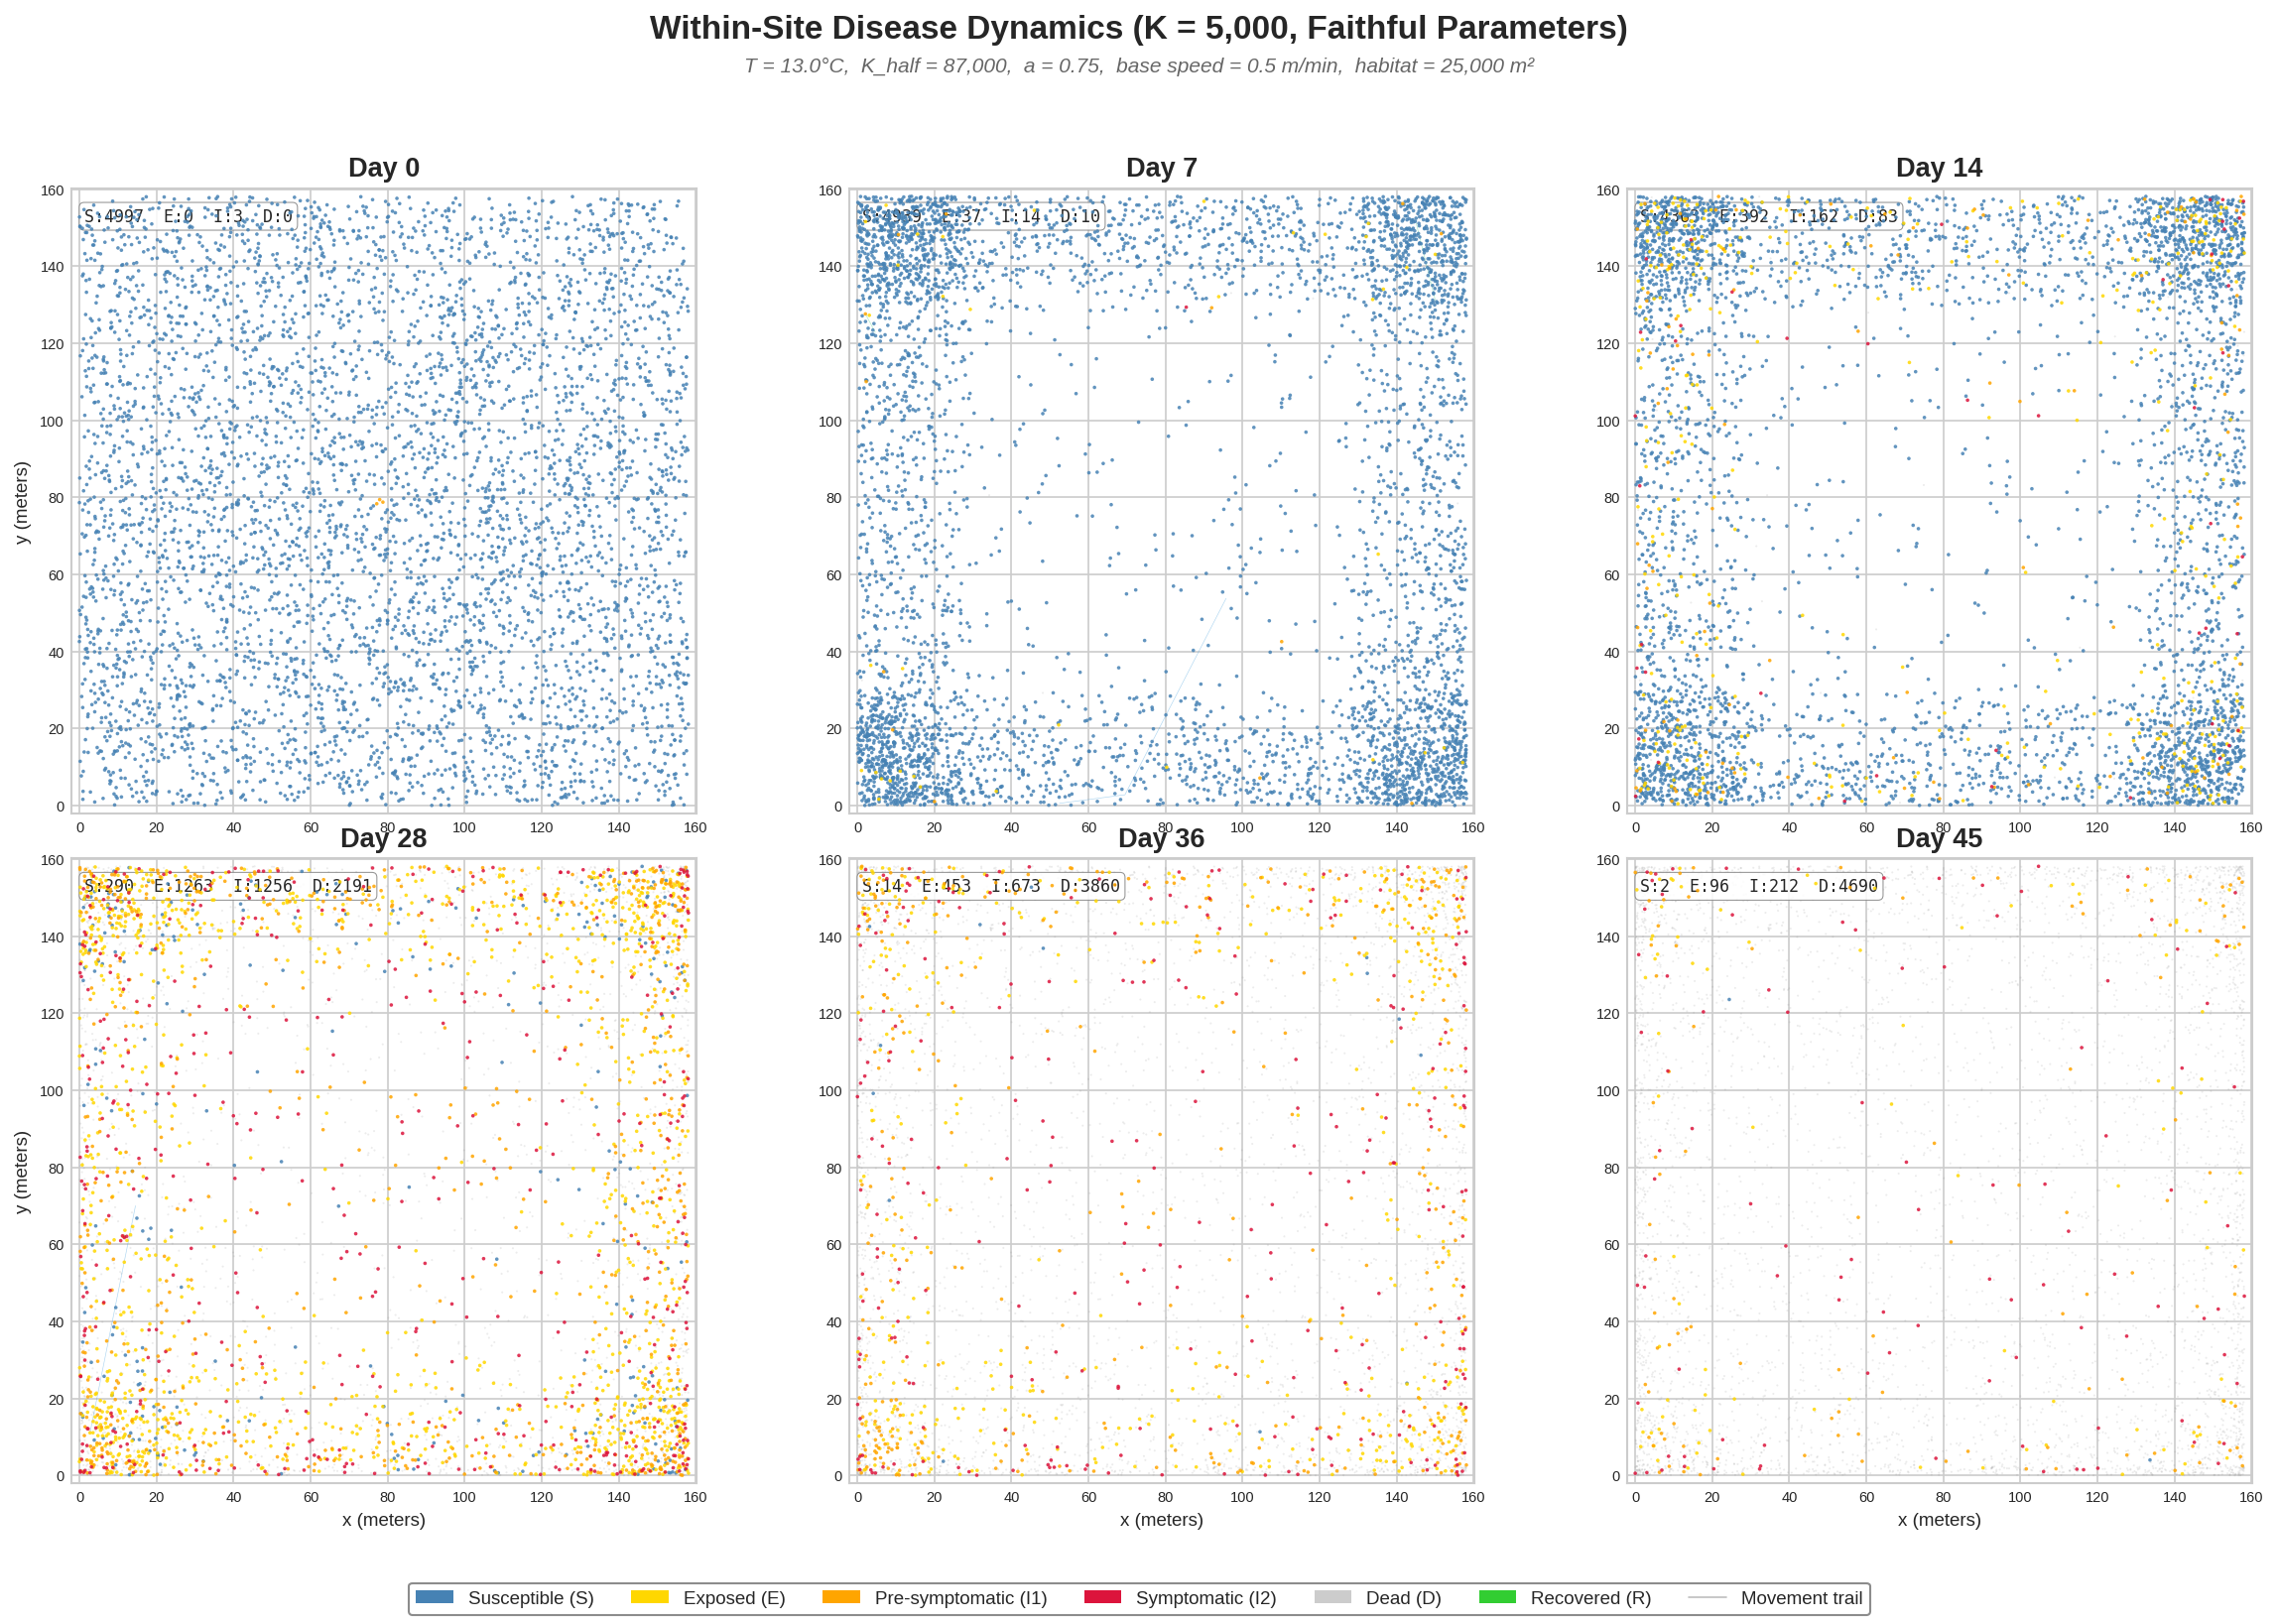
\includegraphics[width=0.95\textwidth]{figures/fig_within_site_disease.png}
    \caption{Simulated within-site disease dynamics using the model's actual spatial transmission mechanics ($K = 5{,}000$ individuals, 158$\times$158~m habitat, $T = 13$\textdegree C). Disease begins with 3 pre-symptomatic individuals (Day~0). By Day~14, exposed (gold) and infected (orange/red) individuals are spreading through spatial proximity effects. Day~28 is peak infection (1,256 active infected). By Day~45, 93.8\% of the population is dead. Zero individuals recovered, consistent with the very low initial recovery ability ($\bar{c} = 0.02$). The rapidity of collapse at high density contrasts with only $\sim$12\% mortality at low density, illustrating the density-dependent positive feedback in pathogen dynamics.}
    \label{fig:within_site_disease}
\end{figure}

\paragraph{Wavefront propagation.}
Consistent with observational records, disease originates from five sites
in the Channel Islands (southern California) in mid-2013 and spreads as a
northward wave.  Three mechanisms interact to produce the wavefront:
(1)~thermal activation requires SST to exceed $T_\mathrm{vbnc}$ before the
pathogen can establish locally, so southern sites ignite first;
(2)~a cumulative dose threshold of 1{,}000 units must be reached before
local outbreak onset, creating a realistic lag between first exposure and
epizootic; and (3)~waterborne pathogen disperses between connected sites
via an exponential decay kernel ($D_P = 300$\,km characteristic distance),
allowing the disease front to propagate along the coast.

% --- Figure: Disease Wavefront Snapshots (from progress report) ---
\begin{figure}[!htbp]
    \centering
    
\includegraphics[width=0.95\textwidth]{figures/fig_disease_snapshots.png}
    \caption{Four snapshots of the range-wide disease simulation. \textbf{Top left:} Pre-disease (2012), all populations near carrying capacity. \textbf{Top right:} Peak crash (2014--2015), disease spreading northward from southern California. \textbf{Bottom left:} Mid-simulation (2016--2017), partial recovery in Alaska driven by seasonal pathogen dormancy. \textbf{Bottom right:} Final state (2024), showing the persistent north--south gradient in population survival.}
    \label{fig:disease_snapshots}
\end{figure}

% --------------------------------------------------------------------------
\subsection{Host Genetics and Evolution}
\label{sec:host_genetics}

Each individual carries \textbf{51 diploid genetic loci} divided equally
among three heritable defense traits, inspired by genome-wide association study (GWAS) results from the
congener \textit{Pisaster ochraceus} \citep{schiebelhut2018}---the only
Pacific asteroid for which disease-associated genomic data currently exist.
No equivalent GWAS has yet been conducted for \textit{Pycnopodia}.

\begin{description}
  \item[Resistance ($r$, 17 loci):] Scales the individual's infection
    hazard rate by $(1-r)$.  A star with $r = 0.30$ experiences a 30\%
    reduction in its instantaneous infection risk per unit pathogen
    exposure.  Think of it as an \textit{armor rating}.

  \item[Tolerance ($t$, 17 loci):] Extends survival during symptomatic
    (I$_2$) infection, reducing the rate of progression to death.  A
    tolerant star lives longer while infected, buying time for possible
    clearance.

  \item[Recovery ($c$, 17 loci):] Scales the daily probability of
    clearing the pathogen.  Effective daily clearance is
    $\rho_\mathrm{rec} \times c$, where $\rho_\mathrm{rec} = 0.05$.
    Cleared individuals return to susceptible status (R$\to$S; no
    adaptive immunity in echinoderms).
\end{description}

Locus effect sizes follow an exponential distribution (a few loci of large
effect, many of small effect), and traits are computed as additive sums
across their respective loci.  Initial trait values---$r_0 = 0.15$,
$t_0 = 0.10$, $c_0 = 0.02$---reflect a largely na\"ive population prior to
the 2013 outbreak.  At $c_0 = 0.02$, the effective daily clearance rate is
just 0.1\%, meaning recovery from active infection is extremely rare.

\paragraph{Natural selection.}
Selection operates straightforwardly: individuals that survive disease
disproportionately carry favorable alleles at defense loci.  When survivors
reproduce, they pass those alleles to offspring.  Over generations, mean
defense trait values increase.  By 2050, resistance in hard-hit southern
populations rises from 0.15 to approximately 0.43, while
less-affected northern populations evolve more slowly ($r \approx 0.20$--0.25).
However, even $r = 0.45$ still leaves more than half of the pathogen force
unblocked---evolution is real but not a rescue.

A critical secondary effect is \textbf{genetic diversity loss}.  Populations
that crash to near-zero lose most of their standing genetic variation.
The additive genetic variance ($V_A$) for resistance in southern
California---the raw material for future adaptation---collapses from
0.026 to 0.003, an 88\% reduction.  The populations most in need of
continued evolution have the least capacity for it.

% --------------------------------------------------------------------------
\subsection{Pathogen Community Evolution}
\label{sec:pathogen_evo_model}

Rather than tracking individual bacterial strains, the model treats the
pathogen community at each site as the evolutionary unit---an aggregate
whose properties shift in response to local selection pressures.  Each
community has two evolving traits:

\paragraph{Thermal activation threshold ($T_\mathrm{vbnc}$).}
The temperature midpoint for the VBNC sigmoid drifts downward at cold-water
sites where there is sustained selection for cold-tolerant strains.  In
Alaska, the community threshold evolves from 12\textdegree C to approximately
9.0--9.4\textdegree C over the simulation, extending the active disease
season by several weeks.  At warm southern sites, where the pathogen is
already active year-round, the threshold barely changes---there is no
selection pressure for further cold adaptation.  Evolution of this trait is
bounded by a hard biophysical floor at 9\textdegree C.

\paragraph{Local virulence ($v_\mathrm{local}$).}
Virulence evolves according to the classic virulence--transmission trade-off
\citep{anderson1982}.  A more virulent pathogen kills hosts faster,
generating larger pathogen bursts, but also terminates shedding sooner.  The
optimal strategy depends on local conditions: in warm, high-density
environments, high virulence is favored (quick kill, many available hosts);
in cold, sparse environments, lower virulence is favored (host kept alive
longer, maximizing total transmission during a brief warm window).  Each
site's community drifts toward a local optimum, producing a latitudinal
gradient from $v \approx 0.08$ in Alaska to $v \approx 0.35$ in Baja
California.

The combination of thermal adaptation and virulence evolution creates
distinct pathogen strategies across the range: northern communities are
\textit{more cold-tolerant but less virulent}, while southern communities
are \textit{already warm-adapted but highly aggressive}.

% --------------------------------------------------------------------------
\subsection{Reproduction and Dispersal}
\label{sec:reproduction}

\paragraph{Broadcast spawning.}
Sunflower stars reproduce via broadcast spawning, releasing eggs and sperm
into the water column.  Spawning timing follows a latitude-dependent
schedule (peak spawning day $= 50 + 3 \times [\text{latitude} - 48.5^{\circ}]$),
with the season running from November through March \citep{hodin2021}.
Alaskan populations spawn later (mid-March) than Californian populations
(mid-January).

\paragraph{Sweepstakes reproductive success.}
Reproductive output follows the Hedgecock sweepstakes hypothesis
\citep{hedgecock2011}: in any spawning event, a small fraction of adults
contribute disproportionately to the next generation.  We implement this
as a Pareto-weighted random lottery (shape $\alpha = 1.35$), where each
reproductive adult receives a random weight from a heavy-tailed distribution.
This amplifies genetic drift, reduces effective population size ($N_e$)
well below the census count, and means that recovery genetics depend
heavily on \textit{which} individuals happen to win the reproductive
lottery---not just how many survive.

\paragraph{Larval dispersal.}
Larvae disperse between connected sites via an exponential decay kernel
with characteristic distance $D_L = 400$\,km.  Rather than modeling
hydrodynamic transport, we use a simplified connectivity scheme weighted by
overwater distance between sites and modified by coastal geometry.  Settler
survival is 0.1\%---consistent with the extremely high larval mortality
typical of marine invertebrates.

\paragraph{Allee effects.}
The model incorporates a \textbf{double Allee effect} at depleted sites.
First, fertilization success depends on local adult density via
Lundquist--Botsford kinetics ($F(\rho) = 1 - e^{-\gamma \rho_\mathrm{eff}}$,
$\gamma = 4.5$\,m$^2$): at low density, eggs fail to encounter sperm.
Second, larval settlement success follows a Michaelis--Menten curve from
20\% (substrate cues only) to 100\% (full adult chemical cues), so sites
with few adults are difficult for larvae to recolonize.  Together, these
mechanisms create an extinction vortex at very low densities---directly
relevant to reintroduction planning, where release cohorts must be large
enough to overcome both thresholds.

Pre-spawning aggregation behavior partially mitigates the fertilization
Allee effect: for 14 days before and after spawning, individuals' movement
is biased toward nearby conspecifics within a 100\,m detection range,
raising effective local density in clumps.

\paragraph{The enclosedness metric.}
A novel feature of the model is an algorithmic measure of each site's
geographic enclosure based on surrounding coastline geometry.  Sites deep
within fjords or inland seas score high; exposed outer-coast headlands score
low.  Enclosedness controls an inherent trade-off:
\begin{itemize}
  \item \textbf{Larval retention} increases at enclosed sites (good for
    recovery---local reproduction contributes more to local recruitment).
  \item \textbf{Pathogen retention} also increases (bad for disease
    escape---the same physical barriers that trap larvae trap waterborne
    \textit{Vibrio}).
\end{itemize}
Per-site flushing rates are computed as $\varphi = f(\text{enclosedness},\;
n_\mathrm{conn} = 0.3)$, with the nonlinear exponent $n_\mathrm{conn}$
calibrated to balance these opposing effects.  Self-recruitment fractions
interpolate continuously from 2\% (open coast) to 70\% (deep fjord).

% --------------------------------------------------------------------------
\subsection{Calibration Summary}
\label{sec:calibration}

The production model (designated \textbf{W154}) was selected after 154
iterative calibration rounds, each testing different parameter combinations
against empirical data.  Two classes of targets were used:

\begin{description}
  \item[Disease arrival timing:] 17 regional targets for when SSWD was first
    documented, from the Channel Islands (mid-2013) to Alaska (2015--2016),
    drawn from published case reports and monitoring programs.
  \item[Recovery fractions:] Fractional population recovery at each region by
    $\sim$2024.  The initial crash magnitude is well constrained by published
    survey data \citep{gravem2021, gehman2025}, but no consolidated range-wide
    assessment of current \textit{Pycnopodia} population status exists.
    Recovery targets were therefore estimated through expert consultation with
    field researchers across the species' range, synthesizing unpublished dive
    survey data and researcher experience into order-of-magnitude targets
    spanning 50\% (Prince William Sound, substantial cold-water recovery) to
    0.1\% (northern California, near-extirpation).  See
    Appendix~\ref{sec:appendix_targets} for details.
\end{description}

Overall fit is quantified by the \textbf{log-RMSE} (root-mean-square error
of log-transformed recovery fractions), which weights relative errors equally
across the four-order-of-magnitude range of targets.  W154 achieves a
three-seed mean RMSE of \textbf{0.504} (best single seed: 0.479).

Key calibrated parameters:
\begin{center}
\small
\begin{tabular}{llp{8cm}}
\toprule
\textbf{Parameter} & \textbf{Value} & \textbf{Interpretation} \\
\midrule
$K$ & 5{,}000 & Per-site carrying capacity \\
$K_\mathrm{half}$ & 800{,}000 & Environmental pathogen for 50\% infection rate \\
$\alpha_\mathrm{env}$ & 0.18 & Fraction of host shedding entering persistent pool \\
$\delta_\mathrm{env}$ & 0.02/d & Environmental pathogen decay rate \\
$n_\mathrm{conn}$ & 0.3 & Enclosedness-to-flushing nonlinearity \\
$D_P$ & 300\,km & Waterborne pathogen dispersal distance \\
$D_L$ & 400\,km & Larval dispersal distance \\
\bottomrule
\end{tabular}
\end{center}

\paragraph{Known limitation.}
The model's main calibration challenge is Alaska.  W154 produces 2--7\%
recovery in Prince William Sound and Fairweather against 50\% survey-based
targets.  This tension reflects a fundamental model constraint:
strengthening the cold-water reprieve enough to allow 50\% Alaskan recovery
tends to also permit unrealistic recovery at mid-latitude sites.  We note
this transparently as the primary axis of model uncertainty and discuss its
implications in Section~\ref{sec:discussion}.

% --------------------------------------------------------------------------
\subsection{SST Projections}
\label{sec:sst_projections}

Future temperatures (2026--2050) are generated via a \textbf{delta method}
applied to CMIP6 ensemble projections:

\begin{equation}
  T_\mathrm{site}(y, m) \;=\; T_\mathrm{site,clim}(m) \;+\;
  \bigl[\, T_\mathrm{ref,proj}(y, m) - T_\mathrm{ref,baseline}(m) \,\bigr]
\end{equation}

\noindent where $T_\mathrm{site,clim}(m)$ is the site's observed monthly
climatology (2012--2025 mean), $T_\mathrm{ref,proj}(y, m)$ is the CMIP6
projection at the nearest reference site, and $T_\mathrm{ref,baseline}(m)$
is the corresponding CMIP6 historical baseline.  Eleven CMIP6 reference
sites distributed at regular latitudinal intervals map onto the 896 model
sites via nearest-neighbor assignment.  A stochastic daily perturbation
term calibrated to observed interannual SST variance is superimposed to
maintain realistic thermal variability.

Two climate pathways are used:
\begin{description}
  \item[SSP2-4.5 (moderate):] Coast-wide mean warming of approximately
    $+$0.8\textdegree C by 2050 relative to the 2012--2020 baseline, with
    stronger warming in the Gulf of Alaska and weaker warming along the
    upwelling-dominated California Current.
  \item[SSP5-8.5 (high):] Approximately $+$1.5\textdegree C coast-wide,
    with pronounced high-latitude amplification.
\end{description}

This approach preserves each site's local temperature character (seasonal
cycle, interannual variability) while applying the secular warming trend
from the CMIP6 ensemble.  Its main limitation is spatial coarseness: 11
reference points cannot capture fine-scale features such as local upwelling
intensification or freshwater-driven thermal anomalies in fjords.


% ============================================================
% SECTION 6: Discussion
% ============================================================
% ==============================================================================
% Section 6: Discussion
% ==============================================================================

\section{Discussion}
\label{sec:discussion}

\subsection{Recovery without intervention}

Across all four forecast scenarios, the model predicts that
\textit{Pycnopodia helianthoides} populations will stabilize at
approximately 94--95\% below pre-disease levels through mid-century
(F01: 94.6\% decline; F04: 94.2\% decline).  No combination of climate
trajectory and evolutionary capacity produces meaningful coast-wide
recovery to pre-disease abundance.  The absolute population floor shifts
by tens of thousands of individuals between scenarios, but the
qualitative conclusion is unchanged: the species' new normal is a
small fraction of its former abundance.

The mechanism underlying this result is what we term the
\textbf{seasonal disease ratchet}.  During winter, falling water
temperatures push \textit{V.\ pectenicida} into VBNC dormancy,
disease pressure abates, and surviving adults reproduce.  Larval
recruitment partially replenishes depleted sites.  But each summer,
rising temperatures reactivate the pathogen, the environmental pool
rebuilds through the shedding--infection positive feedback, and newly
recruited cohorts are culled alongside the survivors.  The net effect
is a population that oscillates around a low equilibrium, gaining
recruits in winter and losing them in summer, unable to escape the
ratchet.  This pattern is especially pronounced from Washington
southward, where summer SST consistently exceeds the VBNC activation
threshold and disease activity spans 6--10 months of the year.

\subsection{The Oregon oasis paradox}

Oregon presents a complex case study in episodic recovery dynamics. 
While 2050 endpoint snapshots suggest 17.6\% of pre-disease capacity 
is retained under F01, the 5-year average reveals only 5.4\% with 121\% 
coefficient of variation---indicating boom-bust cycles rather than 
sustained recovery. Alaska's Fairweather-North region shows more 
reliable persistence (6.8\% endpoint, 9.4\% 5-year average). 
Nevertheless, Oregon's episodic peaks demonstrate what is possible 
under favorable conditions.  Three
features converge to favor Oregon:

\begin{enumerate}
  \item \textbf{Temperature regime.}  Oregon's SST occupies a Goldilocks
    zone---warm enough that the growing and reproductive season is
    adequate for population maintenance, but cool enough that the
    pathogen enters dormancy for several months each winter.  The final
    pathogen thermal threshold at Oregon sites ($T_\mathrm{vbnc} \approx
    10.7$\textdegree C) reflects moderate cold-adaptation, but winter
    SST still drops well below this value, providing genuine disease
    respite.

  \item \textbf{Open-coast flushing.}  Oregon's exposed outer coast
    scores low on the enclosedness metric, yielding high flushing rates
    that continuously dilute the environmental pathogen pool.  Unlike
    the semi-enclosed waters of Puget Sound or British Columbia's fjords,
    where pathogen concentrations build in poorly flushed basins, Oregon's
    sites experience continuous hydrodynamic renewal.

  \item \textbf{Moderate virulence.}  The local pathogen community has
    evolved to intermediate virulence ($v_\mathrm{local} \approx 0.14$),
    low enough that hosts survive long enough to reproduce between
    outbreaks, but high enough that the disease exerts meaningful selection
    for resistance.  Oregon populations have evolved resistance to
    $r \approx 0.38$ by 2050---high enough to meaningfully slow infection
    acquisition.
\end{enumerate}

Under high-end warming (SSP5-8.5, F04), Oregon's episodic booms diminish  
(endpoint drops to 10.4\%) because warmer summers extend the pathogen
activity window.  This underscores that Oregon's oasis dynamics are
thermally mediated and climate-contingent.  For conservation managers,
Oregon represents a double-edged opportunity: its episodic booms 
demonstrate recovery potential and provide valuable monitoring targets, 
but the underlying boom-bust volatility means Oregon cannot be relied 
upon for stable long-term persistence. Alaska's Fairweather regions 
may offer more reliable reintroduction prospects.

\subsection{Alaska's conditional optimism}

Alaska presents a more complicated picture.  The model predicts only
2--10\% recovery for Alaskan regions across climate scenarios, but
we know this is an underestimate: field surveys document substantially
higher recovery in Prince William Sound (estimated ${\sim}$50\%;
\citep{gehman2025}).  The model's Alaskan underprediction is its
single largest calibration shortcoming (Section~\ref{sec:calibration})
and likely reflects processes not fully captured in the current
framework---including freshwater surface lenses that suppress
\textit{Vibrio} in fjord environments, localized upwelling, or
higher background cold-tolerance in northern host genotypes.

Setting aside the absolute numbers, the model's \textit{directional}
prediction for Alaska is noteworthy.  Under SSP5-8.5, Fairweather
North recovery increases from 6.8\% (F01) to 9.9\% (F04)---a 45\%
relative improvement.  Warming extends the growing season and
reproductive window in cold-water Alaskan habitats without
proportionally extending the disease season, because SST in these
regions remains near or below the VBNC floor for much of the year
even under high emissions.  If real Alaskan populations are indeed
doing substantially better than the model shows, then climate
change---paradoxically---may create further opportunity for northern
populations by expanding favorable thermal habitat.

This has a practical implication: Alaskan populations may be the
species' best long-term reservoir, and monitoring investments in
Prince William Sound and the Fairweather coast are well justified.

\subsection{Southern California as a conservation priority}

At the opposite end of the range, the model delivers an unambiguous
verdict.  Southern California (CA-S) and Baja California retain
effectively zero population across all scenarios (CA-S: 0.01\% recovery,
${\sim}$52 individuals coast-wide; Baja: functionally extinct with zero
individuals).  Central California (CA-C) retains ${\sim}$12\% under
moderate warming but declines to 7.6\% under SSP5-8.5, and this trend
is downward through 2050 with no indication of stabilization.

Year-round pathogen activity, high evolved virulence
($v_\mathrm{local} \approx 0.30$), and the absence of any seasonal disease
respite make natural recovery effectively impossible in these regions.
The environmental pathogen pool never decays to levels low enough for
naïve recruits to survive their first summer.  Even with strong
selection (resistance evolves to $r \approx 0.43$--0.45 in CA-C by 2050),
the host cannot evolve fast enough to escape the pathogen's demographic
trap.

These findings motivate the upcoming F05--F08 reintroduction scenarios,
which will test whether captive-bred juveniles with elevated resistance
can establish self-sustaining populations in southern waters.  Our
results suggest that any reintroduction effort south of Point
Conception will require \textit{sustained} releases over multiple
years, because single-cohort releases will likely be overwhelmed by the
ambient disease pressure before the population can reach densities
sufficient to buffer annual losses.

\subsection{The evolutionary dead end}

One of the most striking---and sobering---results is that natural
selection, while clearly operating, is insufficient to rescue
\textit{Pycnopodia} from SSWD.  Host resistance evolves substantially
in hard-hit populations: central California's mean resistance increases
from $r = 0.15$ to $r = 0.43$ over 38 simulated years, nearly tripling
the individual-level hazard reduction.  Yet $r = 0.43$ still means that
58\% of the pathogen force of infection penetrates the host's defenses.
In a high-pathogen environment, this translates to effective daily
infection probabilities that remain well above 20\%.  Resistance buys
time, not survival.

The fundamental asymmetry is temporal.  \textit{V.\ pectenicida}
can adapt its thermal tolerance and virulence on daily-to-seasonal
timescales through community-level selection among trillions of
bacteria.  The host evolves its defense traits once per generation,
with a minimum generation time of several years and effective
population sizes ($N_e$) reduced far below census counts by
sweepstakes reproduction \citep{hedgecock2011}.  This mismatch means
the pathogen can track environmental changes orders of magnitude faster
than the host can respond.

Compounding this asymmetry, the populations under strongest selection
are also losing the genetic raw material needed for future adaptation.
Additive genetic variance for resistance in central California drops
88\% (from $V_A = 0.026$ to $V_A = 0.003$) as population bottlenecks
eliminate rare alleles.  Southern populations are being driven into an
evolutionary corner: strong selection, but nothing left to select on.

The implication for conservation is clear.  Captive breeding programs
that screen for high-resistance broodstock \citep{hodin2021} and
maintain genetic diversity through managed crosses are not merely
helpful supplements to natural recovery---they may be the \textit{only}
path to re-establishing \textit{Pycnopodia} in the southern half of
its range, where natural selection alone leads to an evolutionary dead
end.

\subsection{Limitations}

We highlight several important caveats:

\begin{itemize}
  \item \textbf{Alaska underprediction.}  As discussed, the model
    produces 2--10\% Alaskan recovery against ${\sim}$50\% field
    estimates.  This is the model's main weakness and likely reflects
    missing local processes (fjord stratification, freshwater lensing)
    that suppress \textit{Vibrio} activity in these environments.

  \item \textbf{Genetic architecture.}  The 51-locus, three-trait
    framework is borrowed from GWAS data on \textit{Pisaster ochraceus}
    \citep{schiebelhut2018}.  The true genetic basis of SSWD resistance
    in \textit{Pycnopodia} is unknown and may involve different numbers
    of loci, epistatic interactions, or trait architectures not captured
    by the additive model.

  \item \textbf{Climate projections.}  The delta method applied to 11
    CMIP6 reference sites cannot capture fine-scale oceanographic
    features---local upwelling intensification, mesoscale eddies, or
    freshwater-driven thermal anomalies---that may meaningfully alter
    SST trajectories at specific sites.

  \item \textbf{Simplified dispersal.}  Larval and pathogen dispersal
    use distance-decay kernels without explicit ocean current data.
    Real connectivity patterns are shaped by coastal currents, seasonal
    reversals, and mesoscale features that our kernels cannot resolve.

  \item \textbf{Single pathogen.}  We model \textit{V.\ pectenicida}
    as the sole disease agent.  The true SSWD etiology may involve
    co-infections, opportunistic secondary pathogens, or microbiome
    dysbiosis that amplifies the primary infection.

  \item \textbf{Resistance as a scalar trait.}  Real disease resistance
    arises from complex immune networks with epistasis, dominance, and
    genotype-by-environment interactions.  Our additive scalar
    approximation captures the broad dynamics of selection but not the
    full complexity of host--pathogen coevolution at the molecular level.
\end{itemize}

\subsection{What comes next}

Three immediate extensions of this work are planned:

\begin{description}
  \item[Reintroduction scenarios (F05--F08):]  We will simulate captive
    breeding releases at depleted southern sites, testing different
    release sizes, frequencies, broodstock resistance levels, and site
    selection strategies.  These scenarios will directly inform the
    operational decisions facing the \textit{Pycnopodia} recovery
    program.

  \item[Sensitivity analysis:]  A formal Morris screening followed by
    Sobol variance-based decomposition will identify which model
    parameters most strongly influence population outcomes.  This will
    focus future calibration effort where it matters most and quantify
    the uncertainty envelope around our forecasts.

  \item[Publication manuscript:]  The present report will be condensed
    and submitted for peer review, providing the broader marine
    conservation community with a quantitative framework for
    \textit{Pycnopodia} recovery planning.
\end{description}

Taken together, the forecast results paint a picture that is challenging
but not hopeless.  Natural recovery alone will not restore
\textit{Pycnopodia} to its former abundance anywhere in its range, and
southern populations face functional extinction without intervention.
But the model also identifies genuine bright spots---Oregon's thermal
refuge, Alaska's cold-water reservoir, and the steady (if slow)
accumulation of resistance alleles in surviving populations---that
provide conservation managers with concrete targets for monitoring,
protection, and eventual reintroduction.


% ============================================================
% ACKNOWLEDGMENTS
% ============================================================
\section*{Acknowledgments}

We thank Jason Hodin and the members of the Sea Star Lab at Friday Harbor Laboratories for ongoing discussions about \textit{Pycnopodia} biology and captive breeding protocols. Sea surface temperature data were provided by the NOAA Optimum Interpolation Sea Surface Temperature (OISST) dataset. Climate projections were derived from CMIP6 model outputs. Computing resources were provided by a dedicated Xeon W-3365 server.

% ============================================================
% APPENDIX: Model Parameters
% ============================================================
\clearpage
% ==============================================================================
% Section 7: Appendix — Model Parameters
% ==============================================================================

\appendix

\section{Region Codes}
\label{sec:appendix_regions}

Table~\ref{tab:regions} maps the abbreviated region codes used throughout this report to their full geographic names.

\begin{table}[ht]
\centering
\caption{Region code glossary. Regions are listed north to south.}
\label{tab:regions}
\small
\begin{tabular}{lll}
\toprule
\textbf{Code} & \textbf{Full Name} & \textbf{Approx.\ Latitude} \\
\midrule
AK-PWS & Prince William Sound, Alaska & 60.5\textdegree N \\
AK-EG & Eastern Gulf of Alaska & 59.5\textdegree N \\
AK-OC & Alaska Outer Coast & 59.0\textdegree N \\
AK-FN & Fairweather North (SE Alaska) & 58.5\textdegree N \\
AK-WG & Western Gulf of Alaska & 57.5\textdegree N \\
AK-FS & Fairweather South (SE Alaska) & 57.0\textdegree N \\
AK-AL & Aleutian Islands & 53.0\textdegree N \\
BC-N & British Columbia North & 54.0\textdegree N \\
BC-C & British Columbia Central & 51.0\textdegree N \\
SS-N & Salish Sea North & 49.0\textdegree N \\
JDF & Juan de Fuca Strait & 48.3\textdegree N \\
SS-S & Salish Sea South & 48.0\textdegree N \\
WA-O & Washington Outer Coast & 47.0\textdegree N \\
OR & Oregon & 44.5\textdegree N \\
CA-N & California North & 40.5\textdegree N \\
CA-C & California Central & 36.5\textdegree N \\
CA-S & California South & 34.0\textdegree N \\
BJ & Baja California & 30.0\textdegree N \\
\bottomrule
\end{tabular}
\end{table}

\section{Model Parameters}
\label{sec:appendix_params}

Table~\ref{tab:params} lists all model parameters used in the W154 production configuration. Parameters marked with $\dagger$ were actively varied during the 154-round calibration process.

\small
\begin{longtable}{p{3.2cm} p{1.3cm} p{1.5cm} p{7cm}}
\caption{Complete model parameters for the W154 production configuration.}
\label{tab:params} \\
\toprule
\textbf{Parameter} & \textbf{Symbol} & \textbf{Value} & \textbf{Description} \\
\midrule
\endfirsthead
\toprule
\textbf{Parameter} & \textbf{Symbol} & \textbf{Value} & \textbf{Description} \\
\midrule
\endhead
\midrule
\multicolumn{4}{r}{\textit{Continued on next page}} \\
\endfoot
\bottomrule
\endlastfoot

\multicolumn{4}{l}{\textbf{Disease Transmission}} \\
\midrule
Exposure coefficient & $a_{\text{exp}}$ & 0.75 & Efficiency of environmental pathogen translating to infection risk \\
Half-saturation$^\dagger$ & $K_{\text{half}}$ & 800,000 & Environmental pathogen level for 50\% of maximum dose--response \\
Pathogen activation & $T_{\text{vbnc}}$ & 12\textdegree C & Temperature above which dormant \textit{Vibrio} become infectious \\
VBNC steepness & $k_{\text{vbnc}}$ & 2.0 & Sigmoid sharpness around $T_{\text{vbnc}}$ \\
Thermal floor & $T_{\text{vbnc,min}}$ & 9\textdegree C & Lowest temperature pathogen can evolve to activate at \\
\midrule

\multicolumn{4}{l}{\textbf{Environmental Pathogen Pool}} \\
\midrule
Background input & $P_{\text{env,max}}$ & 2,000 & Maximum background \textit{Vibrio} production (bact/mL/d) \\
Accumulation$^\dagger$ & $\alpha_{\text{env}}$ & 0.18 & Fraction of host shedding entering persistent pool \\
Decay rate & $\delta_{\text{env}}$ & 0.02 & Daily environmental pathogen degradation (2\%/d, $t_{1/2} \approx 35$~d) \\
Pool floor & $P_{\text{floor}}$ & 500 & Minimum pathogen maintained at active sites \\
\midrule

\multicolumn{4}{l}{\textbf{Wavefront Spread}} \\
\midrule
Origin sites & --- & 5 & Channel Islands nodes where SSWD first appeared (2013) \\
Dose threshold & CDT & 1,000 & Cumulative pathogen dose to trigger local outbreak \\
Dispersal range & $D_P$ & 300~km & Characteristic waterborne pathogen dispersal distance \\
Max dispersal & $D_{P,\text{max}}$ & 3,000~km & Maximum long-range pathogen transport \\
\midrule

\multicolumn{4}{l}{\textbf{Disease Progression}} \\
\midrule
Pre-symptomatic shedding & $\sigma_1$ & 5.0 & Pathogen shed rate, I$_1$ stage \\
Symptomatic shedding & $\sigma_2$ & 50.0 & Pathogen shed rate, I$_2$ stage (10$\times$ higher) \\
Death shedding & $\sigma_D$ & 15.0 & Pathogen burst on host death \\
E$\to$I$_1$ rate & $\mu_{EI_1}$ & 0.233/d & Exposed to pre-symptomatic (at 20\textdegree C) \\
I$_1$$\to$I$_2$ rate & $\mu_{I_1 I_2}$ & 0.434/d & Pre-symptomatic to symptomatic \\
I$_2$$\to$Death rate & $\mu_{I_2 D}$ & 0.563/d & Symptomatic to death \\
Recovery rate & $\rho_{\text{rec}}$ & 0.05 & Base daily clearance probability ($\times$ individual $c$) \\
\midrule

\multicolumn{4}{l}{\textbf{Pathogen Evolution}} \\
\midrule
Thermal adapt rate & --- & 0.001/d & Speed of thermal threshold drift \\
Virulence adapt rate & --- & 0.001/d & Speed of virulence drift \\
Max virulence & $v_{\text{max}}$ & 0.70 & Upper virulence bound \\
\midrule

\multicolumn{4}{l}{\textbf{Host Genetics}} \\
\midrule
Resistance loci & $n_R$ & 17 & Loci controlling infection hazard reduction \\
Tolerance loci & $n_T$ & 17 & Loci controlling I$_2$ survival extension \\
Recovery loci & $n_C$ & 17 & Loci controlling pathogen clearance \\
Initial resistance & $\bar{r}_0$ & 0.15 & Starting hazard reduction (85\% susceptible) \\
Initial tolerance & $\bar{t}_0$ & 0.10 & Starting tolerance \\
Initial recovery & $\bar{c}_0$ & 0.02 & Starting clearance scalar ($\times \rho_{\text{rec}} = 0.001$/d) \\
Tolerance ceiling & $\tau_{\text{max}}$ & 0.85 & Maximum survival extension fraction \\
\midrule

\multicolumn{4}{l}{\textbf{Reproduction}} \\
\midrule
Peak spawning day & --- & Day 50 & Peak at reference latitude (48.5\textdegree N) \\
Latitude shift & --- & 3~d/\textdegree & Spawning shifts later with latitude \\
SRS Pareto shape & $\alpha_{\text{SRS}}$ & 1.35 & Reproductive skew (lower = more sweepstakes-like) \\
Settler survival & $s_0$ & 0.001 & Larval survival to juvenile (0.1\%) \\
Post-spawn immuno-suppression & --- & 28~d & Increased susceptibility after spawning \\
\midrule

\multicolumn{4}{l}{\textbf{Spatial Connectivity}} \\
\midrule
Larval dispersal & $D_L$ & 400~km & Characteristic larval dispersal distance \\
Connectivity exponent$^\dagger$ & $n_{\text{conn}}$ & 0.3 & Enclosedness$\to$flushing nonlinearity \\
Self-recruit (open)$^\dagger$ & $\alpha_{\text{open}}$ & 0.02 & Minimum larval retention (exposed coast) \\
Self-recruit (fjord)$^\dagger$ & $\alpha_{\text{fjord}}$ & 0.70 & Maximum larval retention (deep fjord) \\
\midrule

\multicolumn{4}{l}{\textbf{Population Biology}} \\
\midrule
Carrying capacity & $K$ & 5,000 & Maximum population per site (uniform) \\
Max body size & $L_\infty$ & 1,000~mm & Asymptotic arm length (von Bertalanffy) \\
Growth rate & $k_g$ & 0.08/yr & Growth toward max size \\
Min reproductive size & $L_{\text{min}}$ & 400~mm & Minimum size to spawn \\
Natural senescence & --- & 50~yr & Age at increased natural mortality \\
\midrule

\multicolumn{4}{l}{\textbf{Simulation}} \\
\midrule
Start year & --- & 2012 & Simulation start \\
Duration & --- & 38~yr & Total simulation years (2012--2050) \\
Disease onset & --- & Year 1 & Wavefront begins in simulation year 1 (2013) \\
SST transition & --- & 2025 & Switch from OISST observations to CMIP6 projections \\

\end{longtable}
\normalsize

\clearpage
\section{Calibration Targets}
\label{sec:appendix_targets}

The model was calibrated against regional recovery fractions estimated for
approximately 2024 (Table~\ref{tab:targets}).  These targets draw on two
distinct classes of evidence:

\begin{enumerate}
  \item \textbf{Published survey data (pre-$\sim$2020).}  Early post-SSWD
    population assessments, including the comprehensive coastwide decline
    estimates of \citet{gravem2021} (90.6\% global decline, $\sim$97--99\%
    in southern regions, $\sim$87.8\% in the north) and MARINe intertidal
    monitoring, provide quantitative baselines for the initial crash
    magnitude.  Disease arrival timing targets are similarly drawn from
    published case reports and monitoring programs that documented the
    southward-to-northward SSWD wavefront during 2013--2016.

  \item \textbf{Expert inference (post-$\sim$2020).}  No consolidated,
    range-wide survey of current \textit{Pycnopodia} population status
    exists as of 2025.  Recovery fractions for calibration were therefore
    estimated through consultation with field researchers active across
    the species' range, including scientists at NOAA, the University of
    Washington Friday Harbor Laboratories, and the broader SSWD research
    community.  These estimates synthesize unpublished dive survey data,
    anecdotal sighting reports, and researcher experience into
    order-of-magnitude recovery targets.  Because these are informed
    estimates rather than formal survey results, we present them as
    approximate targets spanning four orders of magnitude (50\% down to
    0.1\%) and evaluate model fit using log-transformed RMSE, which
    weights relative accuracy equally across this range.
\end{enumerate}

\noindent This two-tier approach reflects the current state of
\textit{Pycnopodia} monitoring: while the initial crash is well documented
in the literature, the subsequent decade of slow, spatially heterogeneous
recovery has not yet been captured in any comprehensive published
assessment.

\begin{table}[ht]
\centering
\caption{Regional recovery targets used for model calibration.}
\label{tab:targets}
\begin{tabular}{lrll}
\toprule
\textbf{Region} & \textbf{Target (\%)} & \textbf{Source} & \textbf{Basis} \\
\midrule
AK-PWS (Prince William Sound) & 50 & Expert & Dive surveys report substantial recovery \\
AK-FN (Fairweather North) & 50 & Expert & Cold-water remote populations persisting \\
AK-FS (Fairweather South) & 20 & Expert & Partial recovery; warmer than PWS \\
BC-N (British Columbia North) & 20 & Expert & Moderate fjord-coast recovery observed \\
SS-S (Salish Sea South) & 5 & Expert & Limited recovery in semi-enclosed waters \\
JDF (Juan de Fuca Strait) & 2 & Expert & Near-total loss reported \\
OR (Oregon) & 0.25 & Expert & Severe decline, rare sightings \\
CA-N (California North) & 0.1 & Expert & Near-extirpation \\
\bottomrule
\multicolumn{4}{l}{\footnotesize \textit{Expert}: researcher consultation and unpublished survey data; no published range-wide assessment available.} \\
\end{tabular}
\end{table}

The production model (W154) achieves a log-RMSE of 0.504 against these targets. The primary remaining discrepancy is in the Alaskan regions: the model predicts 2--7\% recovery where survey data suggest up to 50\%. This is discussed in Section~\ref{sec:discussion}.

\clearpage
\section{SST Projection Methodology}
\label{sec:appendix_sst}

Sea surface temperature (SST) for 2012--2025 was drawn directly from the NOAA Optimum Interpolation SST (OISST) v2.1 dataset, providing daily satellite-derived temperatures on a 0.25\textdegree\ grid. Each model site was assigned the nearest OISST grid cell.

For 2026--2050, we used the \textbf{delta method} to generate site-specific projections from CMIP6 multi-model ensemble outputs. The approach preserves each site's observed climatological baseline while applying projected warming trends:

\begin{equation}
T_{\text{site}}(y, m) = \bar{T}_{\text{site,obs}}(m) + \left[ T_{\text{ref,proj}}(y, m) - \bar{T}_{\text{ref,base}}(m) \right]
\label{eq:delta}
\end{equation}

\noindent where $\bar{T}_{\text{site,obs}}(m)$ is the site's observed monthly climatology (2012--2024 mean), $T_{\text{ref,proj}}(y, m)$ is the CMIP6 projection for the nearest reference site in year $y$ and month $m$, and $\bar{T}_{\text{ref,base}}(m)$ is that reference site's historical baseline (2012--2024 mean).

Eleven CMIP6 reference sites were selected to span the species' range, from the Aleutian Islands (53\textdegree N) to Baja California (30\textdegree N). Each of the 896 model sites was assigned to its nearest reference site by great-circle distance. Projections were generated under both SSP2-4.5 (moderate emissions, used in F01--F03) and SSP5-8.5 (high emissions, used in F04).

The delta method ensures that each site retains its unique seasonal SST cycle and inter-annual variability structure (from the observational record), with only the long-term warming trend adjusted according to the climate scenario. This approach avoids the biases that arise from using raw CMIP6 output directly at coastal locations, where global climate models often have significant resolution-related errors.


% ============================================================
% BIBLIOGRAPHY
% ============================================================
\bibliographystyle{plainnat}

\begin{thebibliography}{15}

\bibitem[Anderson and May(1982)]{anderson1982}
Anderson, R.M.\ and May, R.M.\ (1982).
\newblock Coevolution of hosts and parasites.
\newblock \textit{Parasitology}, 85(2):411--426.

\bibitem[Gehman et al.(2025)]{gehman2025}
Gehman, A.-L.M.\ et al.\ (2025).
\newblock Fjord refugia from sea star wasting disease: environmental conditions limit pathogen impacts on the sunflower sea star.
\newblock \textit{Proceedings of the Royal Society B}, 292(2039):20242726.

\bibitem[Gravem et al.(2021)]{gravem2021}
Gravem, S.A., Gravier, A., Bayraktarov, E., \ldots\ and Moritsch, M.M.\ (2021).
\newblock Pycnopodia helianthoides.
\newblock \textit{The IUCN Red List of Threatened Species}, e.T178290276A197818455.

\bibitem[Hedgecock and Pudovkin(2011)]{hedgecock2011}
Hedgecock, D.\ and Pudovkin, A.I.\ (2011).
\newblock Sweepstakes reproductive success in highly fecund marine fish and shellfish: a review and commentary.
\newblock \textit{Bulletin of Marine Science}, 87(4):971--1002.

\bibitem[Hodin et al.(2021)]{hodin2021}
Hodin, J., Heyland, A., Mercier, A., \ldots\ and Wahltinez, S.\ (2021).
\newblock Culturing and spawning of the sunflower sea star, \textit{Pycnopodia helianthoides}.
\newblock \textit{Frontiers in Marine Science}, 8:735986.

\bibitem[Liu et al.(2019)]{liu2019}
Liu, J., Deng, Y., Li, L., \ldots\ and Peters, B.M.\ (2019).
\newblock Discovery and control of culturable and viable but non-culturable cells of a distinctive \textit{Vibrio parahaemolyticus}.
\newblock \textit{Food Control}, 112:107153.

\bibitem[Lundquist and Botsford(2004)]{lundquist2004}
Lundquist, C.J.\ and Botsford, L.W.\ (2004).
\newblock Model projections of the fishery implications of the Allee effect in broadcast spawners.
\newblock \textit{Ecological Applications}, 14(3):929--941.

\bibitem[Prentice et al.(2025)]{prentice2025}
Prentice, J.A., Hewson, I., Davy, C.M., \ldots\ and Hodin, J.\ (2025).
\newblock \textit{Vibrio pectenicida} satisfies Koch's postulates as a candidate agent of sea star wasting disease.
\newblock \textit{Nature Ecology \& Evolution}, in press.

\bibitem[Schiebelhut et al.(2018)]{schiebelhut2018}
Schiebelhut, L.M., Puritz, J.B., and Dawson, M.N.\ (2018).
\newblock Decimation by sea star wasting disease and rapid genetic change in a keystone species, \textit{Pisaster ochraceus}.
\newblock \textit{Proceedings of the National Academy of Sciences}, 115(27):7069--7074.

\bibitem[Alizon et al.(2009)]{alizon2009}
Alizon, S., Hurford, A., Mideo, N., and Van~Baalen, M.\ (2009).
\newblock Virulence evolution and the trade-off hypothesis: history, current state of affairs and the future.
\newblock \textit{Journal of Evolutionary Biology}, 22(2):245--259.

\bibitem[Bell(2008)]{bell2008}
Bell, G.\ (2008).
\newblock Selection: The Mechanism of Evolution.
\newblock Oxford University Press, 2nd edition.

\bibitem[Gomulkiewicz and Holt(1995)]{gomulkiewicz1995}
Gomulkiewicz, R.\ and Holt, R.D.\ (1995).
\newblock When does evolution by natural selection prevent extinction?
\newblock \textit{Evolution}, 49(1):201--207.

\bibitem[Reynolds et al.(2007)]{reynolds2007}
Reynolds, R.W., Smith, T.M., Liu, C., \ldots\ and Stokes, D.B.\ (2007).
\newblock Daily high-resolution-blended analyses for sea surface temperature.
\newblock \textit{Journal of Climate}, 20(22):5473--5496.

\bibitem[Huang et al.(2021)]{huang2021}
Huang, B., Liu, C., Banzon, V., \ldots\ and Zhang, H.-M.\ (2021).
\newblock Improvements of the Daily Optimum Interpolation Sea Surface Temperature (DOISST) Version~2.1.
\newblock \textit{Journal of Climate}, 34(8):2923--2939.

\end{thebibliography}

\end{document}
